\documentclass{article}\usepackage[]{graphicx}\usepackage[]{xcolor}
% maxwidth is the original width if it is less than linewidth
% otherwise use linewidth (to make sure the graphics do not exceed the margin)
\makeatletter
\def\maxwidth{ %
  \ifdim\Gin@nat@width>\linewidth
    \linewidth
  \else
    \Gin@nat@width
  \fi
}
\makeatother

\definecolor{fgcolor}{rgb}{0.345, 0.345, 0.345}
\newcommand{\hlnum}[1]{\textcolor[rgb]{0.686,0.059,0.569}{#1}}%
\newcommand{\hlstr}[1]{\textcolor[rgb]{0.192,0.494,0.8}{#1}}%
\newcommand{\hlcom}[1]{\textcolor[rgb]{0.678,0.584,0.686}{\textit{#1}}}%
\newcommand{\hlopt}[1]{\textcolor[rgb]{0,0,0}{#1}}%
\newcommand{\hlstd}[1]{\textcolor[rgb]{0.345,0.345,0.345}{#1}}%
\newcommand{\hlkwa}[1]{\textcolor[rgb]{0.161,0.373,0.58}{\textbf{#1}}}%
\newcommand{\hlkwb}[1]{\textcolor[rgb]{0.69,0.353,0.396}{#1}}%
\newcommand{\hlkwc}[1]{\textcolor[rgb]{0.333,0.667,0.333}{#1}}%
\newcommand{\hlkwd}[1]{\textcolor[rgb]{0.737,0.353,0.396}{\textbf{#1}}}%
\let\hlipl\hlkwb

\usepackage{framed}
\makeatletter
\newenvironment{kframe}{%
 \def\at@end@of@kframe{}%
 \ifinner\ifhmode%
  \def\at@end@of@kframe{\end{minipage}}%
  \begin{minipage}{\columnwidth}%
 \fi\fi%
 \def\FrameCommand##1{\hskip\@totalleftmargin \hskip-\fboxsep
 \colorbox{shadecolor}{##1}\hskip-\fboxsep
     % There is no \\@totalrightmargin, so:
     \hskip-\linewidth \hskip-\@totalleftmargin \hskip\columnwidth}%
 \MakeFramed {\advance\hsize-\width
   \@totalleftmargin\z@ \linewidth\hsize
   \@setminipage}}%
 {\par\unskip\endMakeFramed%
 \at@end@of@kframe}
\makeatother

\definecolor{shadecolor}{rgb}{.97, .97, .97}
\definecolor{messagecolor}{rgb}{0, 0, 0}
\definecolor{warningcolor}{rgb}{1, 0, 1}
\definecolor{errorcolor}{rgb}{1, 0, 0}
\newenvironment{knitrout}{}{} % an empty environment to be redefined in TeX

\usepackage{alltt}
\usepackage{hyperref}
\usepackage{blindtext}
\usepackage{graphicx}
\usepackage{float}
\usepackage{listings}
\usepackage{appendix}
\usepackage{amsmath}
\usepackage{amssymb}
\usepackage{amsfonts}
\numberwithin{equation}{section}
\usepackage{comment}
\usepackage{natbib}
\usepackage[a4paper, total={6in, 8in}]{geometry}

\title{Data Visualisation: Theory and Practice}
\author{Yujie Chu, Pia Fullaondo, Qinqing Li, Jacko Zhou}
\IfFileExists{upquote.sty}{\usepackage{upquote}}{}
\begin{document}



\maketitle 

\newpage
\tableofcontents

\newpage  % Start overview section on a new page

\section*{Overview}

\addcontentsline{toc}{section}{Overview} % Add section to the table of contents

\noindent
Graphical statistics is an indispensable tool in the arsenal of every contemporary data scientist. Primarily, it enables one to delve into data, explore its nuances, and effectively communicate empirical discoveries through visual means. This project aims to provide an overview of modern data visualisation methods, delve into their theoretical underpinnings, and demonstrate the potency of these methodologies using both synthetic and authentic datasets. Computational implementations via dashboards — using Python Dash or R Shiny — are used to showcase the methodologies in practice. Furthermore, the project is aware of the ongoing evolution of novel data visualisation techniques, recognising it as an active area of research (e.g. Rodu and Kafadar, 2022), and thus aims to cover both textbook methods as well as state-of-the-art approaches and open problems.\\

\noindent
The thesis explores the theoretical foundations that underlie various visualisation methodologies, study their mathematical construction, and illustrate their practical application. In particular, while chapter 2 focuses on the theoretical framework of data visualisation, the main body is made up of Chapters 3, 4, and 5. These concentrate on standard implementations of Graphical Statistics for univariate, bivariate, and multivariate datasets respectively. Chapter 3 discusses the Kernel Density Estimate, ROC Curve, and Time Series Analysis. Chapter 4 is focused on the topic of regression, discussing the theory behind Simple Linear Regression followed by LOESS regression. Chapter 5 introduces the model selection method AIC and Multiple Linear Regression, followed by the theoretical foundation of biplots and t-SNE. The final chapter covers active research areas in Graphical Statistics. \\


\noindent
Throughout the thesis, vocabulary referencing the programme R are used. The R package names such as \textit{ggplot2} are italicised, while R commands like \texttt{faceting} are displayed in a teletype font. The R code chunks for each figure in the report can be found in a separate \href{https://github.com/Qinqing-Li/Data-Visualisation-Project/tree/main/code}{GitHub code folder}. \\

\noindent \textbf{Literature and Research}\\ 
\noindent
Data visualisation is an area of interest in numerous method-specific publications. One notable publication is the \href{https://www.tandfonline.com/journals/ucgs20}{Journal of Computational and Graphical Statistics}. This journal publishes ongoing research on the latest techniques in computational and graphical methods in statistics, encompassing data analysis and numerical graphical displays. \href{https://www.sciencedirect.com/journal/spatial-statistics}{Spatial Statistics} publishes articles on the theory and application of spatial and spatio-temporal statistics. \href{https://journal.r-project.org}{The R Journal} publishes research articles in statistical computing that are of interest to R users. These together reveal the vast potential for current and future research in this ever-evolving domain, particularly as our digital landscape and data sphere expand at an accelerated pace.\\

\newpage 

\section{Introduction}

\noindent
This chapter underscores the enduring importance of data visualisation. Case examples both of the influential applications, but also dangerous misuses of data visualisations are showcased and analysed. These are sourced from BBC Ideas \cite{bbcdatavis}. Futhermore, an introduction to the R package \textit{ggplot2} is provided, along with a presentation of the datasets used throughout paper. 

\subsection{Historical Background and Misuses of Data Visualisation}

\noindent This section commences with an examination of two case studies delineating the efficacy and impact of data visualisation, succeeded by an exploration of two instances exemplifying problematic data misuse. The overarching objective is to underscore the significance of data visualisation while concurrently highlighting thenecessity of meticulous attention to detail, particularly in light of the potential for data visualisation to be exploited for malicious purposes.\\
 
\\\textbf{Motivations for Using Data Visualisations — Case 1}

\noindent
Florence Nightingale was not only a social reformer and the founder of modern nursing but also a pioneering statistician. It was her application of data visualisation during the Crimean War that transformed the field of healthcare and pushed for social reform.\\  

\noindent
During the Crimean War, Nightingale recognised that unsanitary hospital conditions were claiming more lives than the battlefield itself. With the help of William Farr, Nightingale created the coxcomb aimed to illustrate the toll of preventable mortality on soldiers, as shown in Figure~\ref{fig:coxcomb}. The coxcomb, resembling an unconventional pie chart, partitioned mortality by causes. Blue indicates preventable deaths, red indicates deaths by wounds, and black indicates other causes. The blue areas outweighed the red and black sections combined, highlighting the disproportionate impact of unsanitary hospital conditions on the mortality rate.

\begin{figure}[H]
    \centering
    \includegraphics[width=0.6\textwidth]{image_reference/Nightingale-mortality.jpg}
    \caption{``Diagram of the causes of mortality in the army in the East" (1858) by Florence Nightingale \cite{graphFN}}
    \label{fig:coxcomb}
\end{figure}

\noindent
Nightingale leveraged the compelling visualisations in her advocacy efforts, presenting them to MPs and government officials who otherwise are unlikely to read or understand statistical reports. She successfully persuaded Queen Victoria, head of the British Army at the time, to allocate funding for the improvement of better conditions in military hospitals.\\

\noindent
\textbf{Motivations for Using Data Visualisations — Case 2}
\\
\noindent
Sometimes, one glance is enough to convey the most powerful idea. Edward Hawkins, a British climate scientist and Professor of climate science at the University of Reading, is renowned for his exceptional data visualisations of climate change.\\

\noindent
In 2018, Edward Hawkins was invited to deliver a lecture on climate change in Wales to an audience with diverse backgrounds. It was important to effectively convey the growing urgency surrounding global warming. To achieve this, he created a chart that used only colours, without any words, titles, or legends, as shown in Figure~\ref{fig:global}. This seemingly simple yet remarkably powerful chart visually illustrated the Earth's warming trend since 1850.

\begin{figure}[H]
    \centering
    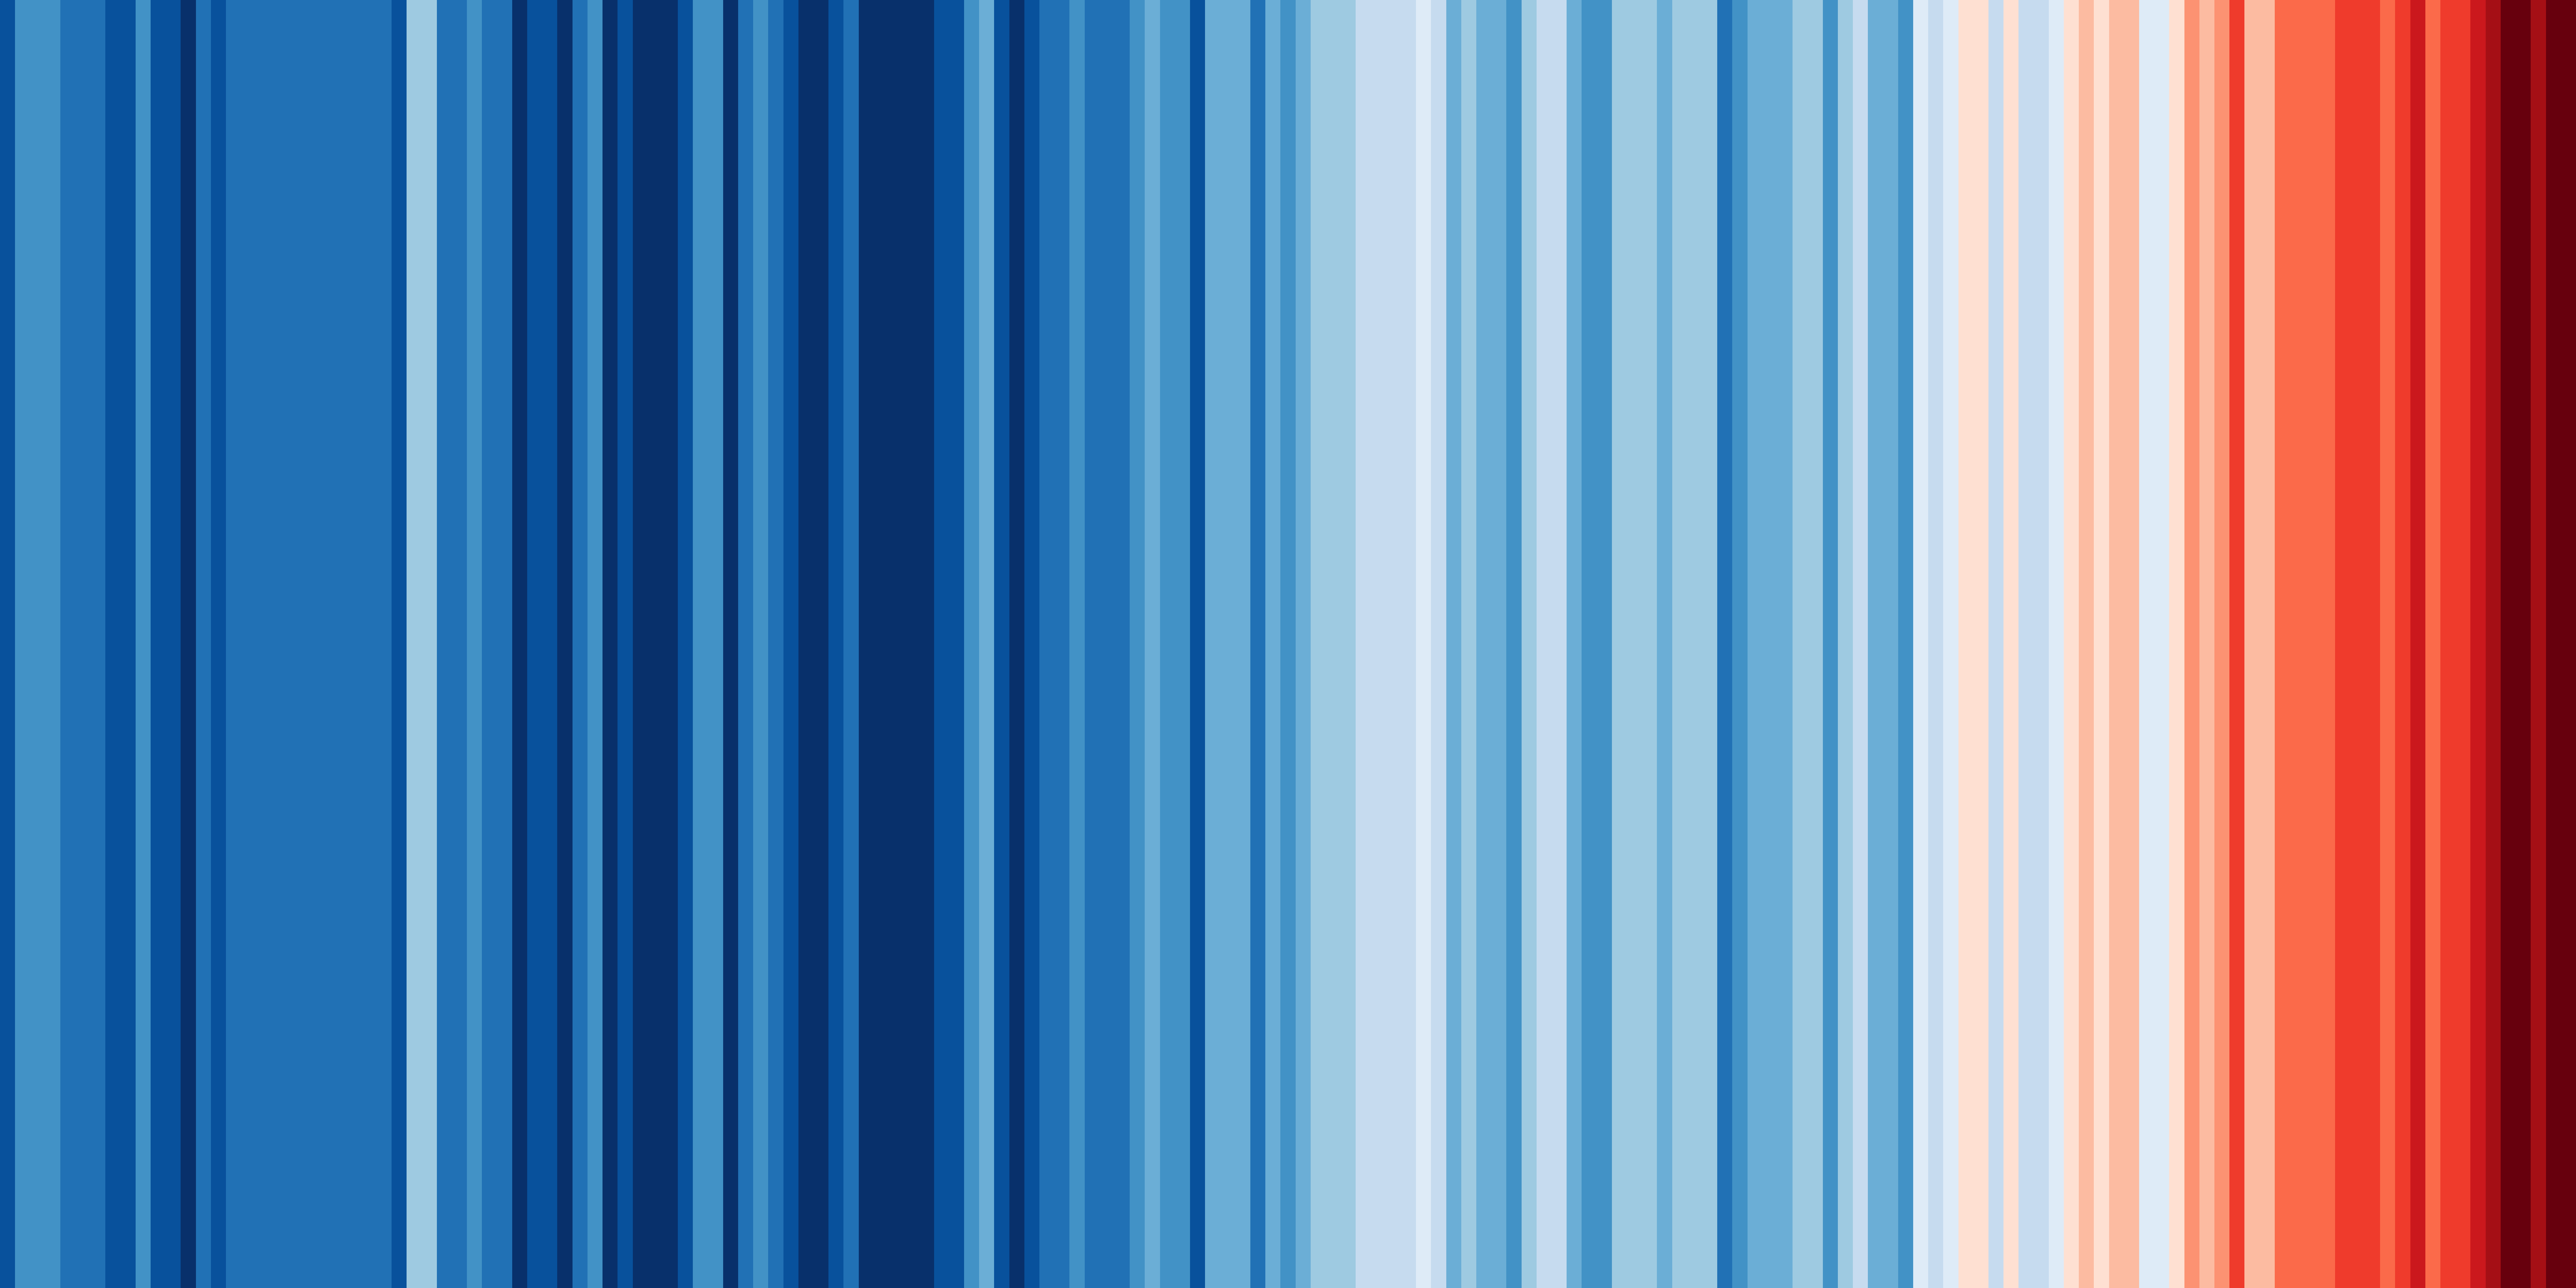
\includegraphics[width=0.6\textwidth]{image_reference/global.png}
    \caption{Latest global stripes (1850-2020) by Edward Hawkins \cite{blog}}
    \label{fig:global}
\end{figure}

\noindent 
Known as the ``warming stripes," this chart cleverly employs blues to indicate cooler-than-average years and reds to signify hotter-than-average years. Its influence reached far and wide, gracing the front pages of major media outlets and featured in news broadcasts worldwide. It became a symbol in climate change demonstrations. Arguably, it stands as one of the most iconic graphics in modern times.\\

\noindent
\textbf{Misuses of Data Visualisation — Case 1}

\noindent
Having observed the remarkable effectiveness of data visualisations, the significance of employing them correctly becomes apparent. The improper use of data visualisations holds the potential to significantly influence the public in misleading ways, resulting in undesired consequences.\\

\noindent
Inappropriate data visualisation can conceal trends rather than reveal them. Figure~\ref{fig:misuse1} illustrates an instance of this issue. On the left-hand side, an inappropriate scale is used - the y-scale ranging from 0 to 30 million dollars, obscuring the fluctuations in payroll spending. Conversely, on the right-hand side, observe that there's a significant increase of over 500,000 dollars in just two months. This revelation is substantial; considering inflation, 500,000 dollars in 1937 is worth well over 10 million dollars today \cite{worth}.

\begin{figure}[H]
    \centering
    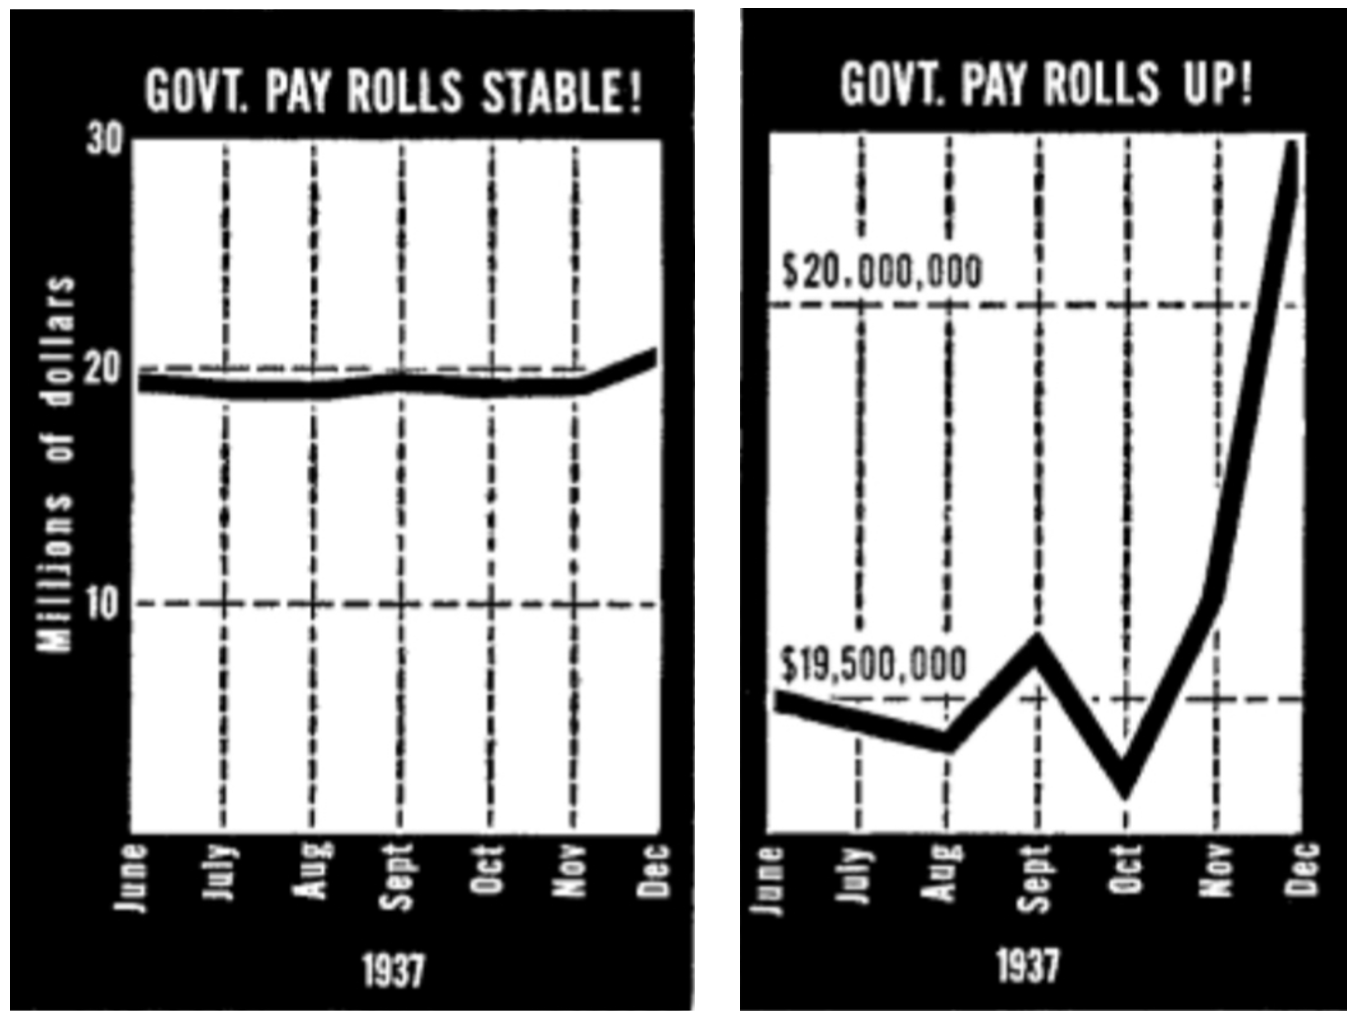
\includegraphics[width=0.6\textwidth]{image_reference/misuse1.png}
    \caption{Incomplete Data Analysis, ``How to lie with statistics" by Miguel de Carvalho \cite{lie}}
    \label{fig:misuse1}
\end{figure}

\noindent 
\textbf{Misuses of Data Visualisation — Case 2}

\noindent
One striking example of data visualisation misuse is found in the Kallikak Family tree - one of the most prominent eugenic narratives of the 20th century.\\

\noindent
The visualisation, shown in Figure~\ref{fig:familytree}, was created by the psychologist Henry Goddard and presented in his 1912 book, ``The Kallikak Family: A Study in the Heredity of Feeble-Mindedness." Goddard's narrative centered around Martin Kallikak, a soldier who, in addition to his marriage to a respected citizen, had a one-night stand with a ``feeble-minded" maid. Goddard believed that intellectual disabilities were inherited traits. In Goddard's account, the legitimate family was successful, while the children of the ``feeble-minded" maid were labeled as ``the lowest types of human beings." However, research has since revealed that the entire story was fictitious, as there was no record of the maid's existence \cite{fakedata}.\\

\noindent
Regrettably, the Kallikak family tree became a central element in the eugenics movement. Figure \ref{fig:familytree} was featured in the 1935 Nazi propaganda film ``Das Erbe" (The Inheritance), which was used to promote public acceptance of Nazi eugenics laws. This propaganda laid the groundwork for the forced sterilization of approximately 400,000 people under Nazi eugenics policies \cite{eugenics}.

\begin{figure}[H]
    \centering
    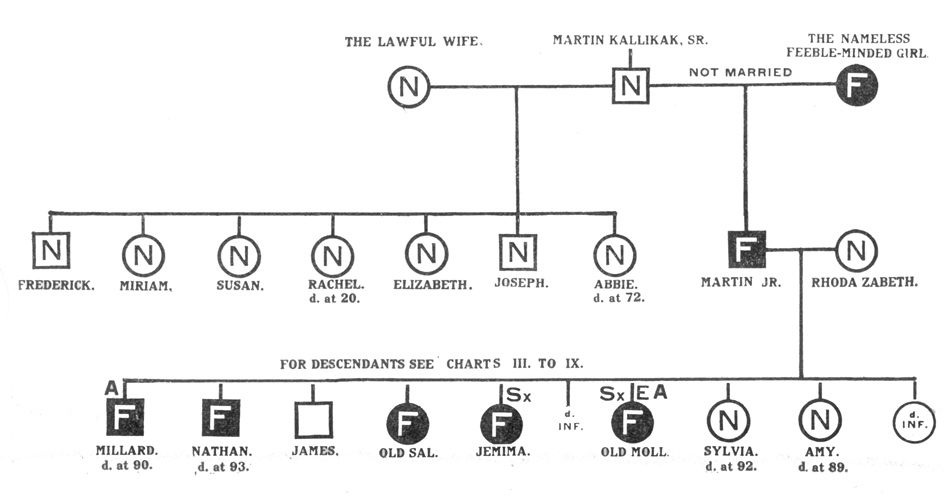
\includegraphics[width=0.7\textwidth]{image_reference/familytree.jpg}
    \caption{The Kallikak Family tree (1912) by Henry Goddard \cite{ktree}}
    \label{fig:familytree}
\end{figure}

\subsection{Computing and Data Visualisation}

As a powerful tool for statistical analysis and graphic creation, R offers a wide array of functionalities to cater to a range of data visualisation needs. In data visualisation, \textit{ggplot2} is the main tool used to create plots capable of representing various types of datasets. The foundation of \textit{ggplot2} lies in the Grammar of Graphics, allowing the sequential construction of individual elements composing a graph, which are subsequently combined to create a unified graphical representation.\\

\noindent\textbf{Key R Commands}\\
\noindent 
As shown in subsequent sections, it is possible to produce visualisations rather effortlessly by utilising internal data from R, or even external data, together with \textit{ggplot2}. When using \textit{ggplot2}, certain key tools are used repeatedly to create visual plots from datasets. Some of these include: \texttt{geom}, \texttt{scale}, \texttt{coord}, \texttt{theme}, and more.\\


\noindent 
These particular tools serve the following functions \cite{ggplot2}: %This section needs to be revised
\noindent
\texttt{geom} refers to geometric objects, pivotal components within \textit{ggplot2} used to define the visual representation of data in a plot. Each \texttt{geom} function corresponds to a specific graphical representation type in a chart. Additionally, in \textit{ggplot2}, \texttt{scales} functions enable the adjustment of various mapping details, including colour choices, label formatting, legend arrangement, and more.\\

\noindent \texttt{coord} provides the axes and gridlines which aid in interpreting the graph. Various coordinate systems such as cartesian, polar, and map projections are available. Furthermore, \texttt{faceting} is a robust feature enabling the partitioning of a single plot into multiple plots based on factors present in the dataset. This functionality proves particularly beneficial for exploring and presenting data with multiple groups or categories.\\

\noindent The \texttt{theme} function holds significance in customising the non-data elements of plots. The theme system within \textit{ggplot2} allows precise adjustment of aesthetic aspects such as fonts, labels, legends, and background colours. This tool is essential for enhancing plot readability and creating visually captivating graphics tailored to specific audiences or publication requirements.\\
\\
\\

\noindent\textbf{Key R Packages}\\
\noindent
The R language is a powerful data analysis tool, and its power lies in the wide variety of R packages that help it achieve a wide variety of functions. Through out this project, different packages, such as $maps$, $dplyr$, $tidyverse$, and $gridExtra$ will be used. These packages significantly enhances the analysis and presentation of data. \\

\noindent
The \textit{dplyr} packages plays a crucial role in data manipulation and transformation. It helps us filter, sort, summarise, and transform datasets, making data analysis more efficient and manageable. The \textit{maps} package is used for providing map data and tools, allowing one to easily draw and display maps in geospatial analyses. The \textit{tidyverse} package is indeed a collection of R packages designed to provide a cohesive and comprehensive set of tools for data science. It includes several widely used packages such as \textit{ggplot2} and \textit{dplyr}. The \textit{gridExtra} packages offers the capability to combine several graphical objects into a cohesive display.\\


\subsection{Datasets}
\noindent
This section introduces the different datasets analysed and visualised in the subsequent chapters.\\

\noindent \textbf{mtcars}: The built-in R dataset, \href{https://www.rdocumentation.org/packages/datasets/versions/3.6.2/topics/mtcars}{mtcars} was extracted from the 1974 Motor Trend US magazine. It includes the fuel consumption and 10 aspects of automobile design for 32 automobiles (1973–74 models). \\

\noindent
\textbf{iris}: The built-in R dataset \href{https://www.rdocumentation.org/packages/datasets/versions/3.6.2/topics/iris}{iris} was collected by Edgar Anderson. This dataset was famously used by British statistician Ronald Fisher to demonstrate linear discriminant analysis in 1936. It encompasses 5 flower characteristics for 3 types of iris, each with 50 samples. \\


\noindent
\textbf{palmerpenguins}: The built-in R dataset \href{https://www.rdocumentation.org/packages/palmerpenguins/versions/0.1.1}{palmerpenguins} was provided by the Palmer Station Long Term Ecological Research. This dataset contains biometric measurements from three distinct penguin species inhabiting the Palmer Archipelago in Antarctica, namely the Adélie, Chinstrap, and Gentoo penguins.\\

\noindent
\textbf{ToothGrowth}: The built-in R dataset, \href{https://www.rdocumentation.org/packages/datasets/versions/3.6.2/topics/ToothGrowth}{ToothGrowth}, measures the tooth growth of 60 guinea pigs. Each animal was either administered with vitamin C or orange juice.\\

\noindent
\textbf{Fire in Brazil}: Open-source fire observation data is provided by \href{https://firms.modaps.eosdis.nasa.gov/}{NASA}. The analysis focuses on Brazil (2013-2022). Note that the dataset contains the variable ``confidence", ranging from 0\% to 100\%. The dataset was filtered with a confidence level of $\ge$ 95\%  to ensure an accurate account of fire occurrences \cite{nasa_confidence}.\\

\noindent
\textbf{Exchange Rate}: The exchange rate data, available at the \href{https://www.bankofengland.co.uk/boeapps/database/index.asp?first=yes&SectionRequired=I&HideNums=-1&ExtraInfo=true&Travel=NIx}{Bank of England}, provides daily spot exchange rates against the pound Sterling (2005-present). This report examines the daily spot rates of the Canadian Dollar, Euro, and US Dollar against the pound Sterling.\\

\noindent
\textbf{Taipei Housing}: The historical real estate valuation from Sindian Dist., New Taipei City, Taiwan,  available at \href{https://archive.ics.uci.edu/dataset/477/real+estate+valuation+data+set}{UC Irvine Machine Learning Repository}.

\newpage 

\section{Theoretical Foundations of Data Visualisation}
This chapter, ``Theoretical Foundations of Data Visualisation," delves into the core principles and concepts that serve as the base of this field. We seek to understand not only the ``how" but also the ``why" behind the creation of visualisations that captivate and inform.

\subsection{Introduction to Data Visualisation Theory}
Creating effective data visualisations requires a robust theoretical framework underlying every chart, graph, or plot. These theoretical underpinnings not only form the basis of data visualisation but also influence how we represent, perceive, understand, and interpret data.\\ 

\noindent \textbf{Guiding Principles for Data Representation}\\
The theoretical framework of data visualisation involves guiding principles dictating visual representation of data. These principles include accuracy, emphasising faithful reflection of underlying data to reduce distortion or misinterpretation; simplicity, advocating for streamlined visuals to convey information effectively; clarity, ensuring visuals are easily understood without unnecessary complexity; relevance, presenting information pertinent to the message or question addressed; and consistency, maintaining uniform use of visual elements like colour coding and labeling throughout a visualisation.\\

\noindent \textbf{Theoretical Framework and Visual Perception}\\
Understanding how the human brain processes visual information is a fundamental aspect of data visualisation theory. This knowledge plays a crucial role in designing visualisations that effectively connect with viewers. It encompasses several key considerations which will be studied in order: the Gestalt Principles, which encompass proximity, similarity, and continuity, affecting how visual elements are grouped and interpreted; Colour Theory, involving the strategic use of colour contrasts and harmonies to improve clarity and impact; and the management of Cognitive Load, which emphasises the importance of reducing mental effort needed to process information.

\subsection{Data Types and Visualisation Techniques}
To have a discussion about data representation, understanding the nature of the data is key. Data comes in various types, and selecting the appropriate visualisation technique is contingent upon recognising these distinctions. In this section, the data types are categorised and matched with their suitable visualisation techniques.

\subsubsection{Categorisation of Data Types}
Data types can be broadly categorised into four main types: 
\begin{itemise}
    \item \textbf{Nominal data}: represents categories or labels without any inherent order. Examples include colours, gender categories, and city names. 
    \item \textbf{Ordinal data}: implies a meaningful order or ranking among categories but lacks equal intervals between them. Examples include survey responses (eg. “very satisfied”, “satisfied”, “neutral”, “dissatisfied”, “very dissatisfied”)
    \item \textbf{Interval data}: possesses ordered categories with equal intervals between them, but it lacks a true zero point. Temperature is measured in Celsius or Fahrenheit as an example. 
    \item \textbf{Ratio data}: includes ordered categories with equal intervals and a meaningful zero point. Examples are age, income, and weight. 
\end{itemise}

\noindent \textbf{Matching Data Types with Appropriate Visualisation Techniques}\\
\noindent Selecting appropriate visualisation techniques is essential for effective data communication. Various data types demand specific visualisation methods for optimal representation \cite{healy2018data}. For nominal data, bar charts and stacked bar charts are effective in displaying categorical information and relative proportions. Ordinal data benefits from ordered bar charts, dot plots, or stacked bar charts, maintaining the ranking and order of categories. Interval data is best visualised using line charts, histograms, and box plots, showcasing trends and distributions without assuming a true zero point. Finally, ratio data finds effective representation through scatter plots, histograms, and line charts, enabling precise comparisons and measurements due to the presence of a meaningful zero point. These are represented in Figure~\ref{fig:data-plots}, where artificial data from a class of 4th-year university students is visualised.

\begin{knitrout}\scriptsize
\definecolor{shadecolor}{rgb}{0.969, 0.969, 0.969}\color{fgcolor}\begin{figure}[H]

{\centering 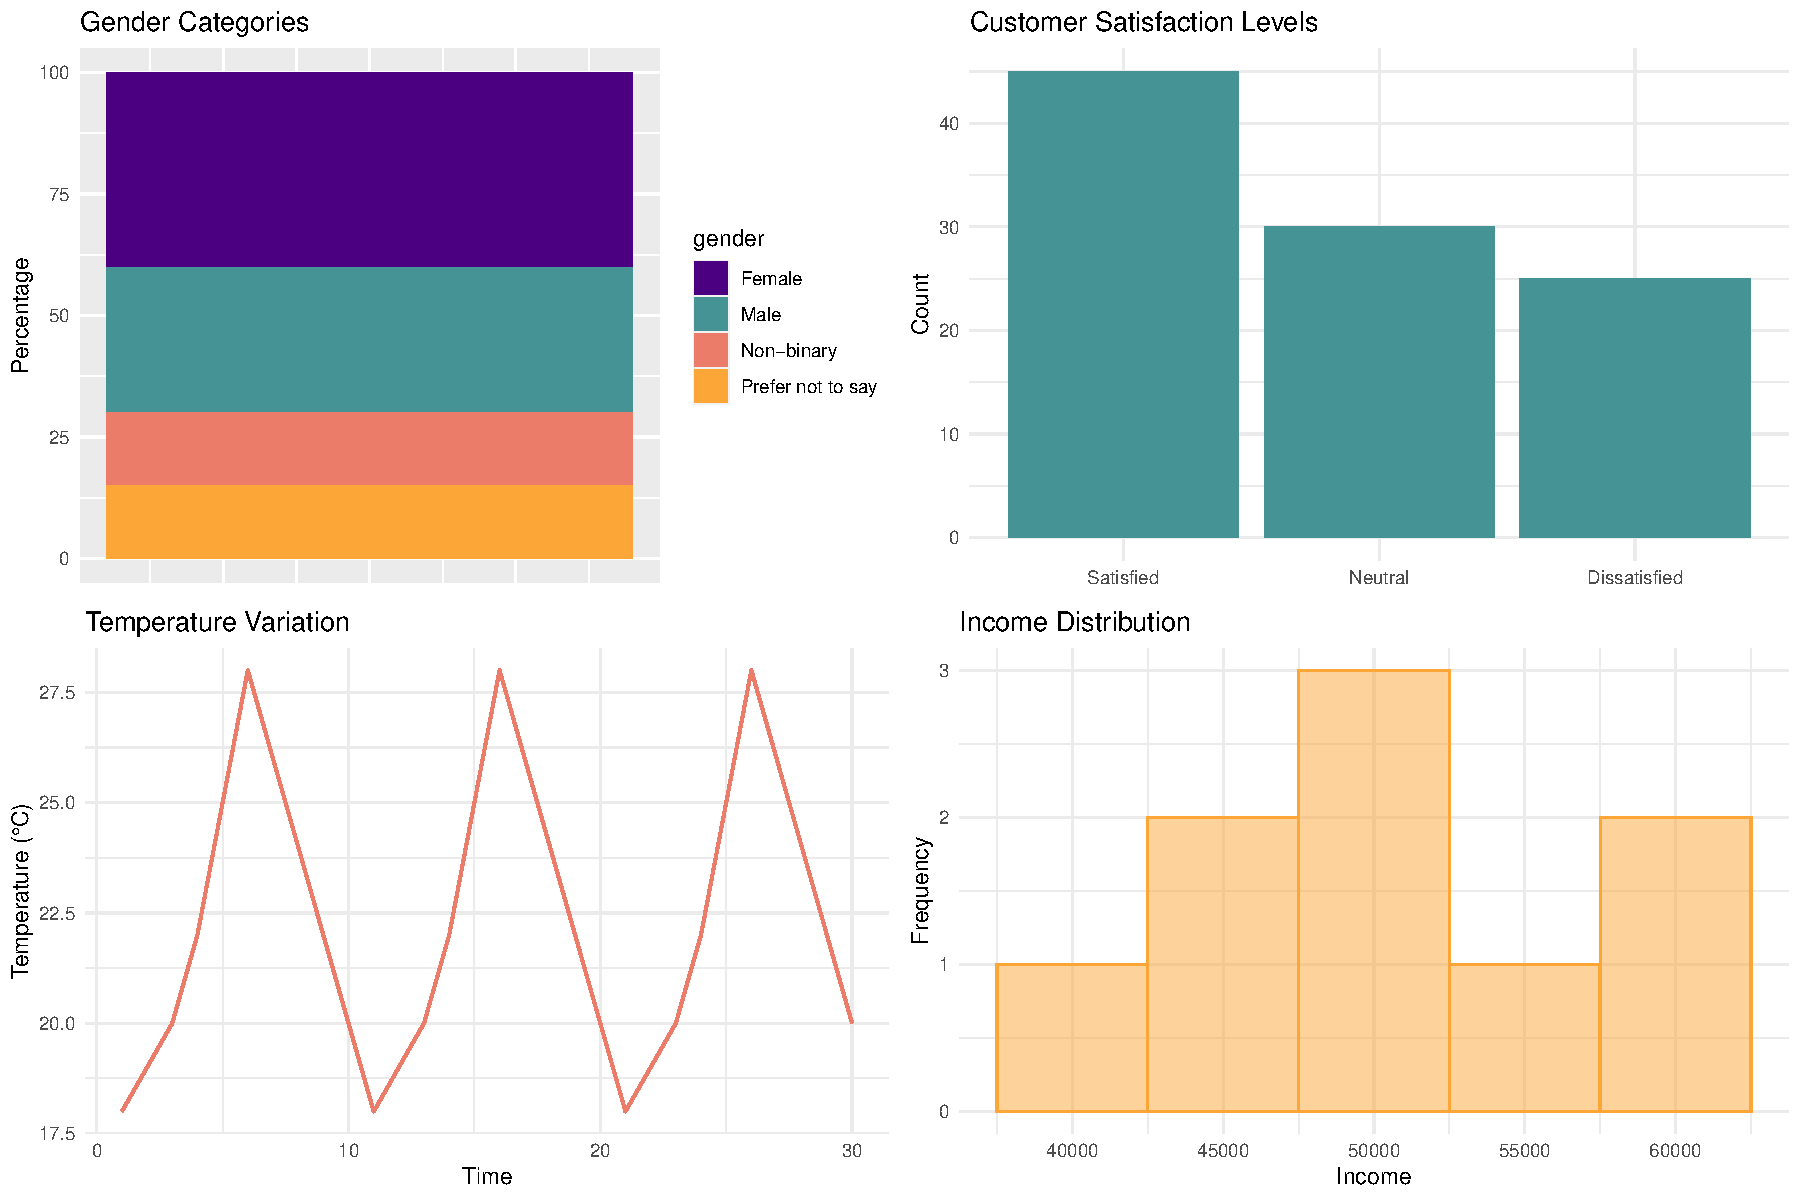
\includegraphics[width=\maxwidth]{figure/beamer-data-plots-1} 

}

\caption[Different types of visualisation techniques according to the data type]{Different types of visualisation techniques according to the data type}\label{fig:data-plots}
\end{figure}

\end{knitrout}
\subsection{Data Abstraction and Representation}
The transformation of raw data into meaningful representations is a pivotal step in data representation. This process, known as data abstraction, involves distilling complex datasets into visual forms that convey insights. In this section, we explore data abstraction, the hierarchies and levels of abstraction in data visualisation, and the critical trade-offs between abstraction and the potential loss of information.\\

\noindent \textbf{Data Abstraction: Transforming Raw Data}\\
Data abstraction involves simplifying and structuring raw data into comprehensible and insightful formats. This process serves as the bridge, transforming numbers, text, and variables into visual elements that convey patterns, trends, and relationships, forming the core of informative data visualisations \cite{tufte2001visual}.

\subsubsection{Hierarchies and Levels of Abstraction}
Abstraction operates on multiple levels of granularity. Hierarchies of abstraction allow us to represent data at varying levels of detail: 
\begin{enumerate}
    \item \textbf{Low-Level Abstraction}: At the lowest level, raw data is preserved in its most detailed form. This might include individual data points, measurements, or unprocessed text.
    \item \textbf{Mid-Level Abstraction}: At the mid-level, data is grouped or aggregated to provide a broader overview. For example, hourly data points may be aggregated into daily or weekly averages.
    \item \textbf{High-Level Abstraction}: At the highest level, data is represented in a condensed and abstracted form, often as summary statistics or key insights. This level provides a big-picture view.
\end{enumerate}

\noindent 
These different levels of abstraction are represented in Figure~\ref{fig:abs-plots}. The first visualisations of the mtcars dataset is a scatter plot that provides detailed information about the relationship between car weight and miles per gallon, with points coloured by the number of cylinders. The second is an abstract visualisation using a box-and-whisker plot to provide a high-level summary of the distribution of miles per gallon for different numbers of cylinders. Finally, the third visualisation is a bar plot presenting aggregated information about the average miles per gallon for different numbers of cylinders.

\begin{knitrout}\scriptsize
\definecolor{shadecolor}{rgb}{0.969, 0.969, 0.969}\color{fgcolor}\begin{figure}[H]

{\centering 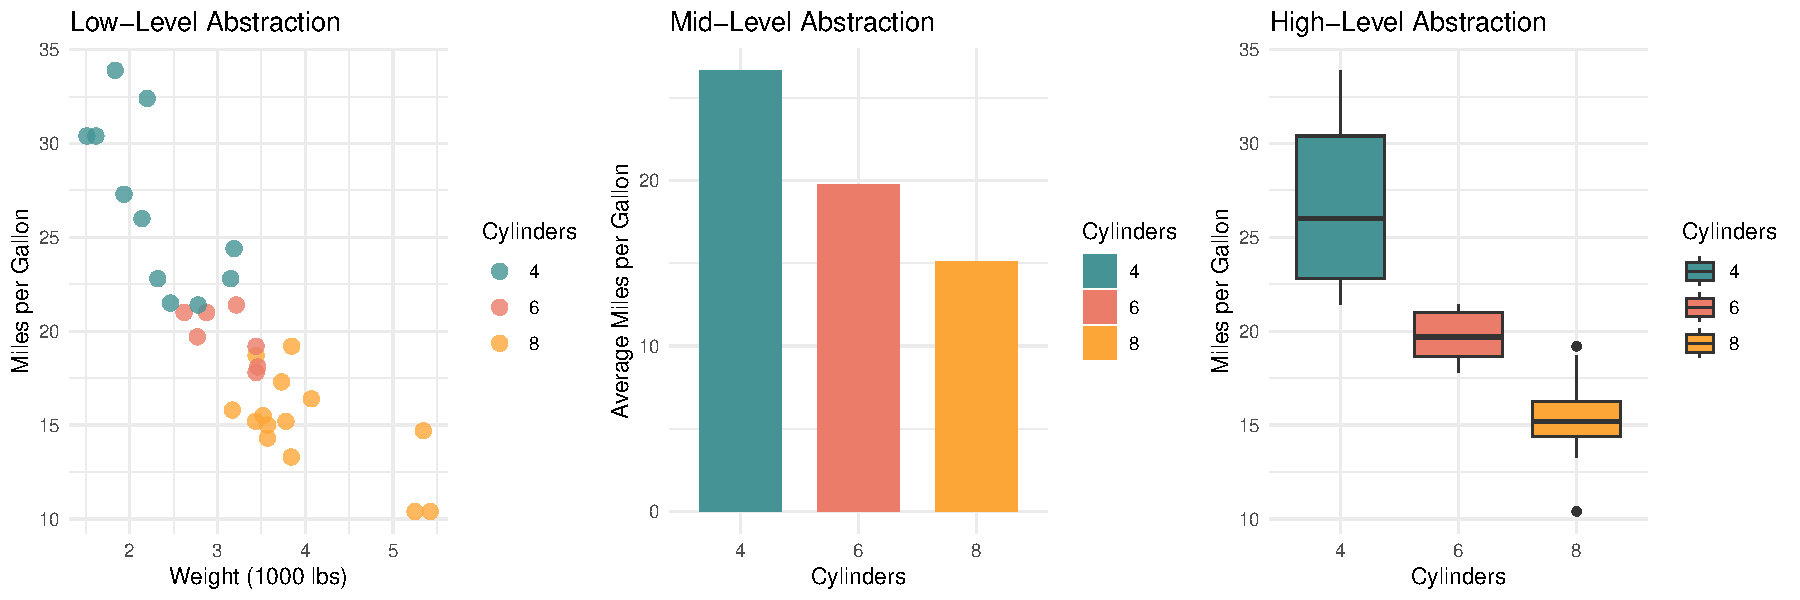
\includegraphics[width=\maxwidth]{figure/beamer-abs-plots-1} 

}

\caption[Mtcars dataset visualised on 3 different levels of abstraction]{Mtcars dataset visualised on 3 different levels of abstraction}\label{fig:abs-plots}
\end{figure}

\end{knitrout}
\\
\\
\noindent \textbf{Trade-offs Between Abstraction and Information Loss}\\
While abstraction simplifies complex data, it presents trade-offs. Designers of data visualisation must strike a balance between clarity and detail, generalisation and specificity, and context versus precision. Abstraction increases clarity but may sacrifice crucial detailed information necessary for some analytical tasks. It offers a more generalised view accessible to a wider audience but might overlook specific nuances essential for experts. While providing valuable context, high-level abstraction may lack the precision required for precise decision-making.\\ 

\noindent 
In data visualisation, the art of data abstraction lies in finding the right level of detail that effectively conveys the intended message while minimising the risk of information loss. This balancing act is a critical consideration in the design of informative and meaningful data visualisations.

\subsection{Visual Perception and Cognition}
In this first section, human visual perception is explored, along with the application of cognitive psychology principles in data visualisation.\\ 

\noindent \textbf{Human Visual Perception: Decoding Visual Information}\\
Human visual perception profoundly influences our understanding of the surrounding world. When applied to data visualisation, it shapes the way that individuals engage with and derive meaning from visual data representations.\\

\noindent 
Significant aspects of human visual perception within data visualisation encompass pattern recognition, adept at identifying trends, outliers, and relationships in data representations. Additionally, perceptual grouping, where visually similar elements are grouped together, influences the interpretation of data clusters and shapes. Moreover, the =hierarchy of perception dictates that certain visual attributes are processed more swiftly and effectively than others, such as colour being processed faster than text, influencing the viewer's attention hierarchy \cite{dastani2002role}.\\

\noindent \textbf{The Gestalt Principles \index{The Gestalt Principles}}\\
Furthermore, the Gestalt Principles play an important role in the realm of visual perception and design \cite{rosli2015gestalt}. Key Gestalt principles crucial in shaping visual information perception include proximity, which groups related elements, similarity that links similar attributes, continuity aiding trend representation, closure for implying connections, and symmetry for balance and aesthetics in visualisations \cite{todorovic2008gestalt}. \\

\noindent By harnessing the principles of human visual perception, applying insights from cognitive psychology, and leveraging pre-attentive attributes, data visualisation designers can create visualisations that are not only aesthetically pleasing but also cognitively efficient.	


\subsection{Colour Theory in Data Visualisation}
In this section, the significance of colour in data visualisation, the principles of colour perception and encoding, and the importance of avoiding misleading visualisations through thoughtful colour choices are explored.\\

\noindent \textbf{The Importance of Colour in Conveying Information}\\
Colour significantly enhances the impact and comprehension of data visualisations. It serves multiple purposes: distinguishing data points, emphasising trends, and offering contextual information. It is utilised to encode categorical data, differentiating between various groups with distinct colours, and to represent quantitative data by using colour intensity or gradients to portray values or magnitudes. Additionally, colour is instrumental in adding context to visualisations through background elements, labels, or annotations, imparting meaning to the data \cite{healy2018data}.\\

\noindent \textbf{Colour Perception and Colour Encoding in Visualisations}\\
Understanding colour perception in data visualisation is crucial. Key principles involve considering colour discrimination, ensuring accessibility for individuals with colour vision deficiencies, as is illustrated by Figure~\ref{fig:colour-plot}. Careful selection of colour schemes aligned with the intended message is essential — for instance, using warm colours like red and orange to indicate caution or warmth, and cool colours like blue and green to convey calmness or coldness. Additionally, attention should be paid to how colours interact when combined; certain combinations might create visual vibrations or impact text legibility.\\

\begin{knitrout}\scriptsize
\definecolor{shadecolor}{rgb}{0.969, 0.969, 0.969}\color{fgcolor}\begin{figure}[H]

{\centering 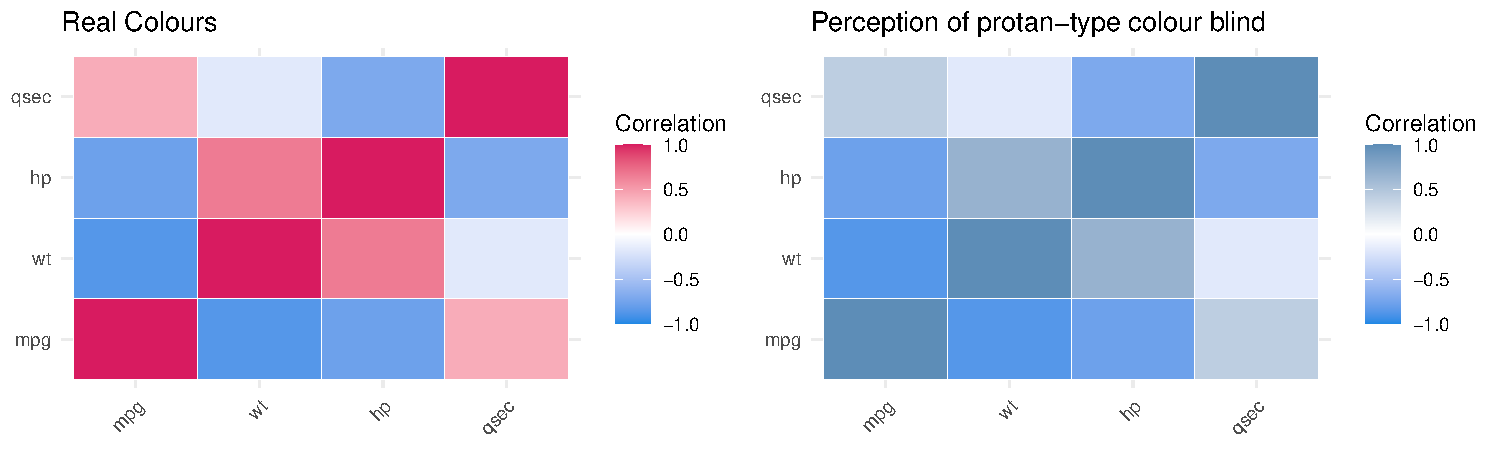
\includegraphics[width=\maxwidth]{figure/beamer-colour-plot-1} 

}

\caption[Colour perception of a heatmap for by a colour blind person]{Colour perception of a heatmap for by a colour blind person}\label{fig:colour-plot}
\end{figure}

\end{knitrout}

\noindent \textbf{Avoiding Misleading Visualisations Due to Colour Choices}\\
Misleading visualisations often stem from inappropriate or deceptive use of colour, requiring precautions to prevent such occurrences. First, maintaining consistency in colour usage throughout the visualisation is essential. Employing a uniform colour scheme for similar data categories or elements helps establish coherence and understanding. Furthermore, it's crucial to avoid colour choices that could distort or exaggerate the data. Overly intense or contrasting colours might mislead interpretations, emphasising the necessity for judicious colour selection.\\

\noindent 
Additionally, providing a clear and concise legend becomes imperative to explain the meaning of colours, especially when dealing with complex or unfamiliar colour schemes. A comprehensive legend helps viewers decipher the represented data accurately.\\


\subsection{Cognitive Load and Visual Complexity}
In data visualisation, achieving a balance between complexity and cognitive load is crucial. Cognitive load significantly influences how viewers engage with and comprehend presented data. Finding a balance is crucial to effectively convey information without overwhelming the viewer's cognitive capacity. This section explores the concept of cognitive load in visualisations, strategies to reduce cognitive load while maintaining complexity, and techniques to combat information overload through simplification.

\subsubsection{Strategies to Reduce Cognitive Load While Maintaining Complexity}
To reduce cognitive load while maintaining complexity in data visualisation, several strategies can be employed. Firstly, establishing a clear visual hierarchy using size, colour, and contrast helps direct attention to crucial elements. Additionally, simplifying labels and text by avoiding unnecessary complexity ensures information is clear and easily digestible.\\

\noindent Furthermore, employing interactive features like tooltips and drill-down functionality assists in providing additional information when required, reducing the density of static visualisations. A final approach involves the use of progressive disclosure, presenting complex information gradually, beginning with an overview and allowing users to explore details as needed.\\

\begin{knitrout}\scriptsize
\definecolor{shadecolor}{rgb}{0.969, 0.969, 0.969}\color{fgcolor}\begin{figure}[H]

{\centering 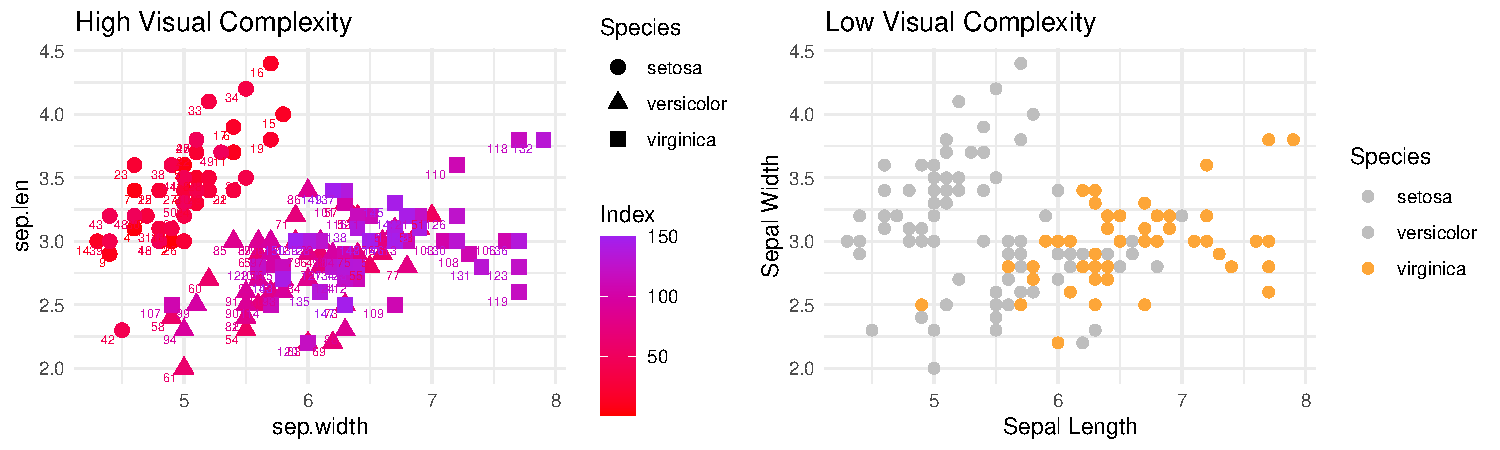
\includegraphics[width=\maxwidth]{figure/beamer-cogload-plot-1} 

}

\caption[High versus low cognitive load demand through the reduction of visual complexity]{High versus low cognitive load demand through the reduction of visual complexity}\label{fig:cogload-plot}
\end{figure}

\end{knitrout}

\subsubsection{Information Overload and Simplification Techniques}
Addressing information overload in visualisations necessitates the strategic application of simplification techniques. Filtering enables focused data selection, while data reduction aggregates information to highlight overarching trends. Storyboarding structures data presentation, aiding in contextual comprehension, and prioritisation ensures critical information is prominently displayed, elevating the visualisation's clarity and impact. These strategies collectively combat overwhelming data or excessive visual elements, enhancing comprehension and the effective communication of insights to viewers.

\newpage

\section{Univariate Data Visualisation Methods}

This chapter, initiates the discussion about data visualisation methods. This chapter particularly introduces techniques for graphically representing for datasets of the simplest nature - that is, single-variable datasets. It focuses on histograms, bar charts, Kernel Density Estimate, ROC Curves, and Time Series Analysis. 

\subsection{Histograms}

A histogram is a graphical representation of the distribution of a dataset. It consists of bars, each representing a range of data values, and whose height corresponds to the frequency or count of data points within that range.In this way, histograms facilitate the visualisation of differences in frequency or quantity among groups.\\

\noindent On a Cartesian coordinate system, the x-axis shows the endpoints of each group, and the y-axis represents frequency. The height of each rectangle indicates the corresponding frequency, making it a frequency distribution histogram. In order to determine the quantity of each group in the histogram, a multiplication of the frequency by the group interval is necessary. Since every histogram has a fixed group interval, if we use the y-axis to directly show quantity and each rectangle's height indicates the number of data points, we can both retain the distribution and simultaneously see the number in each group at a glance. All examples in this text use the non-standard histogram depiction with the y-axis denoting quantity.\\


\subsubsection{Theory of Histogram}\\

\noindent Let \(X_1, \ldots, X_n\) be independent and identically distributed random variables with finite mean \( \mu \) and variance \( \sigma^2 \). Then for any \( \epsilon > 0 \), 
\[ P\left(\left|\frac{1}{n}\sum_{i=1}^n X_i - \mu\right| < \epsilon\right) \rightarrow 1 \] 
as \( n \rightarrow \infty \).\\

\noindent Histograms can be also used to visualise the convergence of sample means to the population mean. Let \(X_1, \ldots, X_n\) be independent and identically distributed random variables with finite mean \( \mu \) and variance \( \sigma^2 \). Define the sample mean \( \bar{X} = \frac{1}{n}\sum_{i=1}^n X_i \). Then, as \( n \) becomes large, the variable 
\[ Z = \frac{\bar{X} - \mu}{\sigma/\sqrt{n}} \] approaches a standard normal distribution.\\

\noindent
\textbf{Classical frequency histogram}\\

\noindent The classical frequency histogram is constructed by dividing the data into a series of nonoverlapping intervals, called bins. The data points within each bin are then counted. The histogram can be fully described by two main factors: the bin width, and the bin origin, $t_{0}$.\\

\noindent
In classical frequency histogram, usually we assume the shape of the histogram to be normal distribution. It is very important to choose the number of bins, since they have a huge impact on how we interpret the data. Too few bins may hide the information in a dataset, and too many bins can cause a lot of noise in a dataset. Fortunately, we can determine the optimal number of bins to use in a histogram by using a method known as Sturges’ Rule:
$$ k = 1 + \log_{2} n, $$

\noindent
where n is the total number of observations in the dataset.\\

\noindent
Technically, Sturges' Rule is method to find the number of bins rather than the width of bins. However, if the data are not normal, additional bins may be needed.\\

\noindent
\textbf{Density Histogram}\\

\noindent
The density histogram is normalized to integrate to 1. Unlike a frequency histogram which is constructed from blocks of height 1 and width $h$ (where $h$ is the fixed bin width), a density histogram is constructed from blocks of height $\frac{1}{nh}$, ensuring that each block has an area equal to $\frac{1}{n}$. The height of each bin  represents the probability distribution of the data, such that the total area of the histogram equals 1.\\

\noindent
\\The density histogram is mathematically defined by the formula:
$$\hat{f}(x) = \frac{v_k}{nh} = \frac{1}{nh} \sum_{i=1}^{n} I_{[t_k,t_{k+1})}(x_i) \quad \text{for } x \in B_k,$$

\noindent
where $v_{k}$ represents the count of sample points falling into the $k$th bin, $B_{k}$. With this definition of a histogram, it is straightforward to check that $ \hat{f}(x) \geq 0 $ and that $ \int \hat{f}(x) \, dx = 1 $, so that $ \hat{f}(x) $ is a proper density function.\\

\noindent
The density histogram's bin counts ${v_{k}}$ can be considered as binomial random variables, where each bin count $v_{k}$ follows a binomial distribution $B(n,p_{k})$. The probability $p_{k}$ for each bin is the integral of the density function $f(t)$ over the bin interval $B_{k}$:
$$p_{k} = \int_{B_k} f(t) \, dt. $$\\

\subsubsection{Histogram in Practice}\\

\noindent The R language uses the \texttt{hist} function to create histograms. This function takes vectors as input, along with other parameters to plot a histogram.\\

\noindent By plotting histograms of a large number of sample means, one can observe the shape gradually resembling a normal distribution.\\

\noindent
Consider Figure~\ref{fig:iris-plots} which was created on \textit{ggplot2} with the use of to the \texttt{geom\_histogram} function and iris dataset.

\begin{figure}[htbp]
  \centering
  \begin{minipage}[b]{0.48\linewidth}
\begin{knitrout}\scriptsize
\definecolor{shadecolor}{rgb}{0.969, 0.969, 0.969}\color{fgcolor}

{\centering 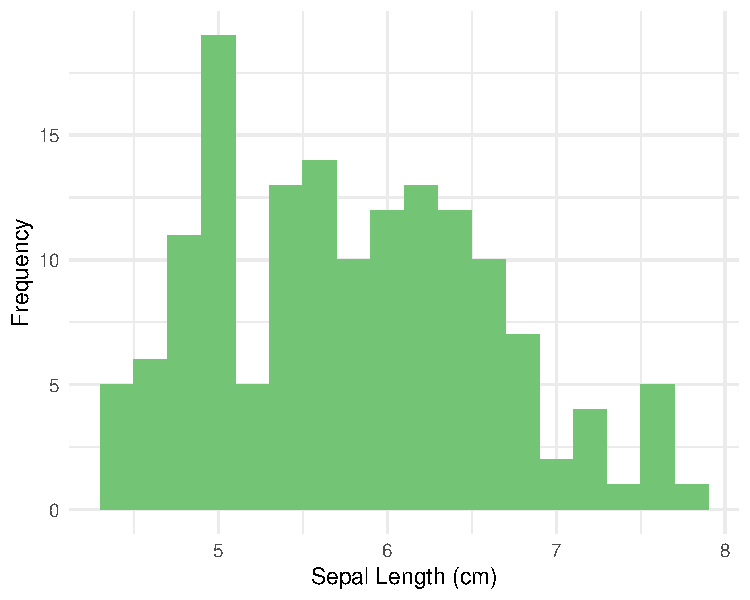
\includegraphics[width=\linewidth]{figure/beamer-hist2-1} 

}


\end{knitrout}
  \end{minipage}
  \hfill
  \begin{minipage}[b]{0.48\linewidth}
\begin{knitrout}\scriptsize
\definecolor{shadecolor}{rgb}{0.969, 0.969, 0.969}\color{fgcolor}

{\centering 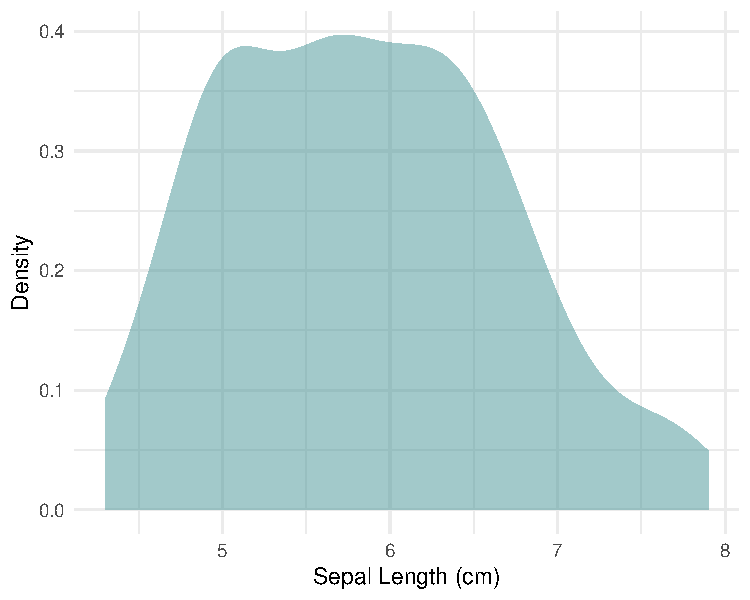
\includegraphics[width=\linewidth]{figure/beamer-kde3-1} 

}


\end{knitrout}
  \end{minipage}
  \caption{Histogram and Kernel Density Estimation of Sepal Length in Iris Dataset}
  \label{fig:iris-plots}
\end{figure}

\subsection{Kernel Density Estimation}

Kernel Density Estimation(KDE) evolves from the concept of histogram, offering a method for estimating the the probability density function of a dataset.

Kernel Density Estimation (KDE) is an very useful tool in statistics. Instead of discrete histograms, it helps create a smooth curve from values in a dataset. KDE is used to infer the distribution of a population based on a limited sample. Thus, the result of the kernel density estimation is an estimate of the sample's probability density function. Based on this estimated probability density function, one can ascertain certain characteristics of the data distribution, such as the regions where data is concentrated.\\

\noindent
The KDE algorithm takes a parameter called bandwidth, that affects how smooth the resulting curve is. Changing the bandwidth changes the shape of the kernel: a lower bandwidth implies only points very close to the chosen position are given any weight, which leads to the estimate looking squiggly. In contrast, a higher bandwidth means having a shallow kernel, where distant points can contribute. Thus, leading to a smoother curve. %REVISE THIS TEXT.
\\

\subsubsection{Theory of Kernel Density Estimation}\\

\noindent
We can express KDE as follows, where the K represent the kernel function:
$$\hat{f}(x) = \sum_{\text{observations}} K\left(\frac{x - \text{observation}}{\text{bandwidth}}\right).$$
In KDE, the variable $x$ represents the point of density estimation. The total number of data points, denoted as $n$, constitutes the sample size, and all these points are used for estimating the dataset's probability density function. The bandwidth $(h)$ is a crucial parameter that controls the smoothness of the estimation, with smaller bandwidths leading to closer fits to data and larger ones smoothing out details. The kernel function $(K)$, such as the Gaussian or triangular kernel, assigns mass around each data point, influencing the density estimate, while $X_i$ represents the individual sample points that collectively contribute to the estimated density function, guided by the kernel function and the bandwidth\cite{wand1994kernel}. Here is the formula for the kernel density estimator:
$$\hat{f}(x; h) = \frac{1}{nh} \sum_{i=1}^{n} K\left(\frac{x - X_i}{h}\right),$$\\
Here, the kernel function \( K(u) \) is a normalized non-negative function that satisfies:
$$ \int K(u) \, du = 1. $$

\noindent
By introducing the rescaling notation $K_h(u) = h^{-1}K(\frac{u}{h})$, we can write the formula in a more compact way:
$$\hat{f}(x; h) = n^{-1} \sum_{i=1}^{n} K_h(x - X_i).$$\\

\noindent In Figure~\ref{fig:iris-plots}, the kernel density estimation of the dataset is presented. The distribution of sepal lengths is depicted by the kernel density curve. The peaks observed in the curve correspond to the primary concentration trends of sepal length within the data. A unimodal curve signifies a concentration of sepal lengths for most irises in that specific region. Conversely, a bimodal or multimodal curve suggests the existence of multiple concentration areas.

\subsection{Bar Charts}
\noindent Bar charts are a crucial tool in data presentation, arranging data into vertical or horizontal bars. The varying lengths of these bars directly correspond to the magnitude of the information they represent. Bar charts excel in comparing classified data, especially when values are closely aligned. This stems from the nature of human perception, as our visual acuity for height surpasses that of other visual elements like area or angle.\\

\noindent Bar charts represent a versatile tool for data visualisation, frequently employed to compare distinct categories. The vertical bar chart, commonly recognised, exhibits categories along the X-axis and their frequencies or counts along the Y-axis. Horizontal bar charts, rotated 90 degrees, prove beneficial for extended category names or numerous categories, displaying categories on the Y-axis and frequencies on the X-axis. Multi-set or grouped bar charts facilitate side-by-side comparisons of sub- groups within categories, available in both vertical and horizontal orientations. Stacked bar charts illustrate classes of values subdivided into sub-classes, often differentiated by colour, where each segment's size signifies its frequency or count, and the total bar length reflects the cumulative total.\\

\subsubsection{Bar Charts in Practice}\\
\noident The two bar charts on in Figure~\ref{fig:barcharts} illustrate the impact of varying vitamin dosages on tooth growth, further categorised by supplement type. On the X-axis, three distinct levels of vitamin dosage are presented, while the Y-axis indicates the average lenth of tooth for each dosage.


\begin{knitrout}\scriptsize
\definecolor{shadecolor}{rgb}{0.969, 0.969, 0.969}\color{fgcolor}\begin{figure}[H]

{\centering 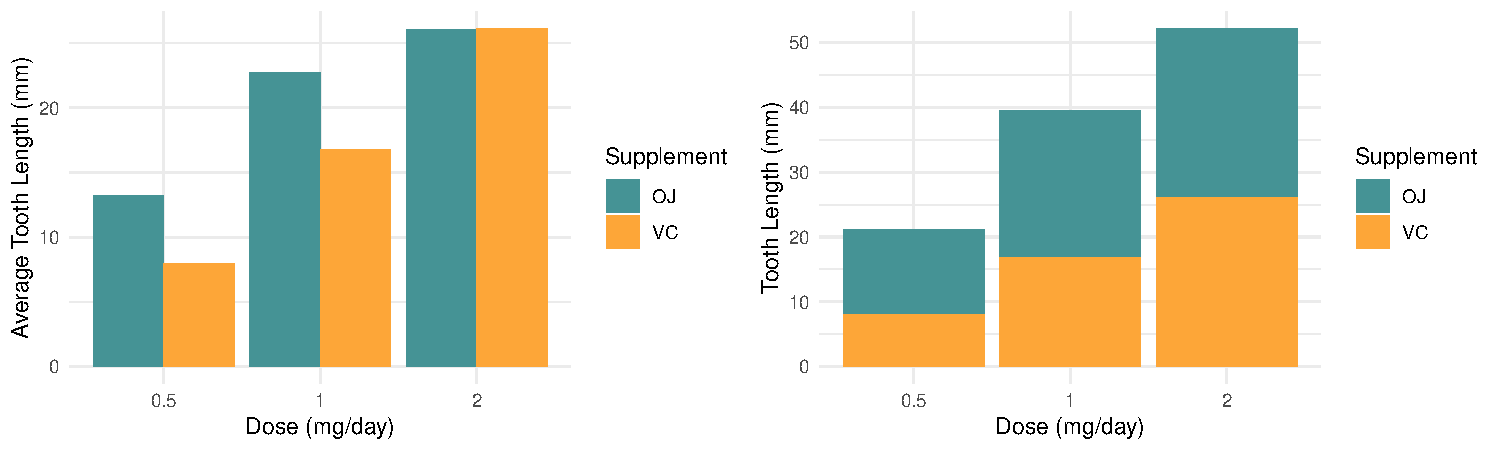
\includegraphics[width=\maxwidth]{figure/beamer-barcharts-1} 

}

\caption[Visualising tooth growth by dosage]{Visualising tooth growth by dosage: A comparison of grouped and stacked bar chart techniques}\label{fig:barcharts}
\end{figure}

\end{knitrout}

\noindent From the grouped bar, chart found on the left of Figure~\ref{fig:barcharts}, due to the side-by-side positioning of the bars, it is easy to note that tooth growth varies not only with the dosage but also with the supplement type. In contrast, the stacked bar graph on the right of Figure~\ref{fig:barcharts} facilitates the understanding of the combined effects of the two supplements at each dosage level. However, compared to the latter, it becomes more challenging to differentiate the individual contribution of each supplement.

\subsection{Line Charts and Time Series}

\noindent
The previous subsections explored Histograms, Kernel Density Estimation, and Bar Charts, which are univariate methods used for analysing independent variables in isolation, revealing patterns and intrinsic properties within data. Now, the focus shifts to univariate methods of dependent variables, specifically Line Charts, which are crucial for visualising relationships between variables to understanding their interactions and dependencies over time.

\subsubsection{Theory of Line Charts}

\noindent
Line charts are fundamental tools in data visualisation, particularly useful for displaying time series data. A line chart represents $n$ data points 
$\{(x_i,y_i)\}_{1 \leq i \leq n}$ on a Cartesian coordinate system, with the x-axis often denoting time intervals or ordered categories and the y-axis representing the measured values.\\ 

\noindent
In a line chart, consecutive data points are typically connected by straight lines. The line segment between two points \((x_i,y_i)\) and \((x_{i+1},y_{i+1})\) can be described by the equation of a line in the slope-intercept form: \(y=mx+b\), where \(m\) is the slope and \(b\) is the y-intercept. Also, a series of linear interpolations between pairs of data points could be used. These interpolations assume that the change between two points is uniform or linear. This linear approach is mathematically represented as:
\[
y = y_i + \frac{y_{i+1} - y_i}{x_{i+1} - x_i} \cdot (x - x_i), \quad  x_i \leq x \leq x_{i+1}.
\]
\noindent
This equation highlights that for any point \(x\) between \(x_i\) and \(x_{i+1}\), the corresponding value of \(y\) on the line chart is determined by a linear relation. This method effectively ``fills the gaps'' between actual observed data points and provides a continuous view of the data.

\subsubsection{Time Series Analysis}\\
\noindent
Time series visualisation is particularly suited to line charts. A time series is a collection of observations $x_t$, where $t$ denotes the time point at which the observation is recorded. An index set $T_0$ which collects all the time points when observations are available. For instance, we often have $T_0 = \{0,\dots ,n\}$ for $n \in \mathbb{N}$. By plotting these data points over time, line charts help in identifying long-term trends, seasonal patterns, and anomalies.\\

\noindent
A time series can be viewed as a realisation of a stochastic process. A stochastic process \cite{Brockwell2016Introduction} $X = (X_t)_{t \in T_0}$ is a collection of random variables $X_t$, where $t$ denotes the time index and $T_0$ the index set. For a fixed event $\omega \in \Omega$ we obtain the realisation of the stochastic process (sometimes also called a sample path) which is given by $x_t = X_t(\omega)$, $t \in T_0$. In practice, line charts of time series data provide insights into the behavior of such stochastic processes over time.\\

\noindent
\textbf{Time Series Visualisation of Exchange rates}\\
\noindent
Here, plot daily and 49-day moving average exchange rates of exchange rate data in one figure.

\begin{figure}[H]
\begin{knitrout}\scriptsize
\definecolor{shadecolor}{rgb}{0.969, 0.969, 0.969}\color{fgcolor}\begin{kframe}
\begin{alltt}
\hlcom{# PLOT OF DAILY AND 49-DAY MOVING AVERAGE EXCHANGE RATES OF CAN, EUR, USD TO GBP}

\hlstd{color_palette} \hlkwb{<-} \hlkwd{c}\hlstd{(}\hlstr{"#459395"}\hlstd{,} \hlstr{"#EB7C69"}\hlstd{,} \hlstr{"#FDA638"}\hlstd{)}

\hlstd{p1} \hlkwb{<-} \hlkwd{ggplot}\hlstd{(plot_dt,} \hlkwd{aes}\hlstd{(}\hlkwc{x} \hlstd{= Date,} \hlkwc{y} \hlstd{= Rate,} \hlkwc{color} \hlstd{= Currency))} \hlopt{+} \hlkwd{geom_line}\hlstd{()} \hlopt{+}
  \hlkwd{labs}\hlstd{(}\hlkwc{y} \hlstd{=} \hlstr{"Exchange Rate to GBP"}\hlstd{,} \hlkwc{x} \hlstd{=} \hlstr{""}\hlstd{,} \hlkwc{color} \hlstd{=} \hlstr{"Currency"}\hlstd{)} \hlopt{+}
  \hlkwd{theme_minimal}\hlstd{()} \hlopt{+} \hlkwd{theme}\hlstd{(}\hlkwc{legend.position} \hlstd{=} \hlstr{"none"}\hlstd{)} \hlopt{+}
  \hlkwd{scale_color_manual}\hlstd{(}\hlkwc{values} \hlstd{= color_palette)}
\hlstd{p2} \hlkwb{<-} \hlkwd{ggplot}\hlstd{(plot_data,} \hlkwd{aes}\hlstd{(}\hlkwc{x} \hlstd{= Date,} \hlkwc{y} \hlstd{= Rate,} \hlkwc{color} \hlstd{= Currency))} \hlopt{+} \hlkwd{geom_line}\hlstd{()} \hlopt{+}
  \hlkwd{labs}\hlstd{(}\hlkwc{y} \hlstd{=} \hlstr{"Exchange Rate to GBP"}\hlstd{,} \hlkwc{x} \hlstd{=} \hlstr{""}\hlstd{,} \hlkwc{color} \hlstd{=} \hlstr{"Currency"}\hlstd{)} \hlopt{+}
  \hlkwd{theme_minimal}\hlstd{()} \hlopt{+} \hlkwd{theme}\hlstd{(}\hlkwc{legend.position} \hlstd{=} \hlstr{"none"}\hlstd{)} \hlopt{+}
  \hlkwd{scale_color_manual}\hlstd{(}\hlkwc{values} \hlstd{= color_palette)}

\hlcom{# Extract the legend and combine the plots }
\hlstd{p2_legend} \hlkwb{<-} \hlstd{cowplot}\hlopt{::}\hlkwd{get_legend}\hlstd{(p2} \hlopt{+} \hlkwd{theme}\hlstd{(}\hlkwc{legend.position} \hlstd{=} \hlstr{"right"}\hlstd{))}
\hlstd{combined_plot} \hlkwb{<-} \hlstd{cowplot}\hlopt{::}\hlkwd{plot_grid}\hlstd{(p1, p2,} \hlkwc{rel_widths} \hlstd{=} \hlkwd{c}\hlstd{(}\hlnum{1}\hlstd{,} \hlnum{1}\hlstd{),} \hlkwc{nrow} \hlstd{=} \hlnum{2}\hlstd{)}
\hlstd{cowplot}\hlopt{::}\hlkwd{plot_grid}\hlstd{(combined_plot, p2_legend,} \hlkwc{nrow} \hlstd{=} \hlnum{1}\hlstd{,} \hlkwc{rel_widths} \hlstd{=} \hlkwd{c}\hlstd{(}\hlnum{2}\hlstd{,} \hlnum{0.5}\hlstd{))}
\end{alltt}
\end{kframe}

{\centering 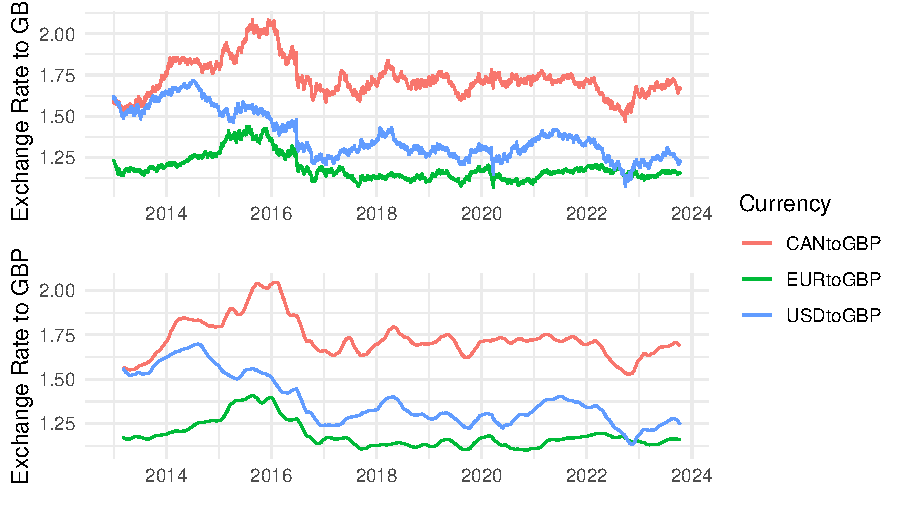
\includegraphics[width=\maxwidth]{figure/beamer-unnamed-chunk-2-1} 

}


\end{knitrout}
\centering
\caption{Daily (top) and 49-day moving average (bottom) exchange rates of CAN, EUR, USD to GBP}
\label{fig:all exchange rates}
\end{figure}

\noindent
The first plot in Figure~\ref{fig:all exchange rates} presents a comparative visualisation of daily exchange rates for CAD, EUR, and USD against GBP, offering an overview of their trends and relative performance. This plot enables the identification of overall trends and periods of volatility for each currency pair, allowing for an assessment of their stability and strength relative to GBP. Notice that, there was a simultaneous and significant drop in all three currencies relative to the GBP. The concurrent nature of these declines across diverse currency pairs suggests that the driving factor is a depreciation of the GBP, rather than independent appreciations of the USD, EUR, and CAN. This notable depreciation of the GBP occurred around 2016, which coincides with the commencement of BREXIT process. Usually, the long term trend attracts financial analyst most. Therefore, filtering fluctuations and anomalies is important. Then, a 49-day moving average (MA49) was employed, shown in the second plot of Figure~\ref{fig:all exchange rates}, to elucidate long-term trends while mitigating short-term fluctuations. This is mathematically represented as 
\[\text{MA}_{49}(t) = \frac{1}{49} \sum_{k=t-48}^{t} x_k,\] 
where \( x_k \) denotes the exchange rate on day $k$.\\

\noindent
This method effectively filters out daily noise, allowing a clearer view of overarching trends in currency movements against the GBP. The overlay of these moving averages on the daily exchange rates in visualisations provides both a clear comparative and a quantitative perspective.\\

\noindent
\textbf{Decomposition of Time Series}\\
\noindent
One of the primary advantages of time series visualisation is the ease with which it allows analysts to identify long-term upward or downward trends in data and patterns that repeat over specific intervals. By decomposing the time series, it would be easy to see those features.\\

\noindent
Time series data, $X_t$, can often be described as a combination of several distinct components: Trend component $t_t$: The underlying progression in the series, Seasonal component $s_t$: Periodic fluctuations due to seasonal factor, Residual $r_t$: The irregular or error component.\\

\noindent
The decomposition of a time series can be described in two main models:
\\

\noindent \textbf{Additive Model} \cite{Brockwell2016Introduction}: In the additive model, the components are added together:
\[
X_t = t_t + s_t + r_t.
\]
\textbf{Multiplicative Model} \cite{Brockwell2016Introduction}: In the multiplicative model, the components are multiplied together:
\[
X_t = t_t \times s_t \times r_t \quad \text{or} \quad \log(X_t) = \log(t_t) + \log(s_t) + \log(r_t).
\]
In practice, the choice between the additive and multiplicative models often depends on the nature of the time series. If the magnitude of the seasonal fluctuations or the variation around the trend does not vary with the level of the time series, then an additive model is appropriate. If the magnitude of the seasonal fluctuations or the variation around the trend increases or decreases as the time series level changes, then a multiplicative model may be more suitable.\\

\noindent
R function \texttt{decompose()} is able to decompose the time series by additive model or multiplicative model. And below is the demonstration of decomposition.




\begin{figure}[H]
\begin{knitrout}\scriptsize
\definecolor{shadecolor}{rgb}{0.969, 0.969, 0.969}\color{fgcolor}\begin{kframe}
\begin{alltt}
\hlcom{# PLOT OF DECOMPOSITION OF ADDICTIVE TIME SERIES MODEL}
\hlkwd{ggplot}\hlstd{(decomposed_df,} \hlkwd{aes}\hlstd{(}\hlkwc{x} \hlstd{= time,} \hlkwc{y} \hlstd{= value))} \hlopt{+} \hlkwd{geom_line}\hlstd{()} \hlopt{+}
  \hlkwd{facet_wrap}\hlstd{(}\hlopt{~}\hlstd{component,} \hlkwc{scales} \hlstd{=} \hlstr{"free_y"}\hlstd{,} \hlkwc{ncol} \hlstd{=} \hlnum{1}\hlstd{)} \hlopt{+} \hlkwd{labs}\hlstd{(}\hlkwc{x} \hlstd{=} \hlstr{"Date"}\hlstd{,}\hlkwc{y} \hlstd{=} \hlstr{"Exchange Rate to GBP"}\hlstd{)} \hlopt{+} \hlkwd{theme_minimal}\hlstd{()}
\end{alltt}
\end{kframe}

{\centering 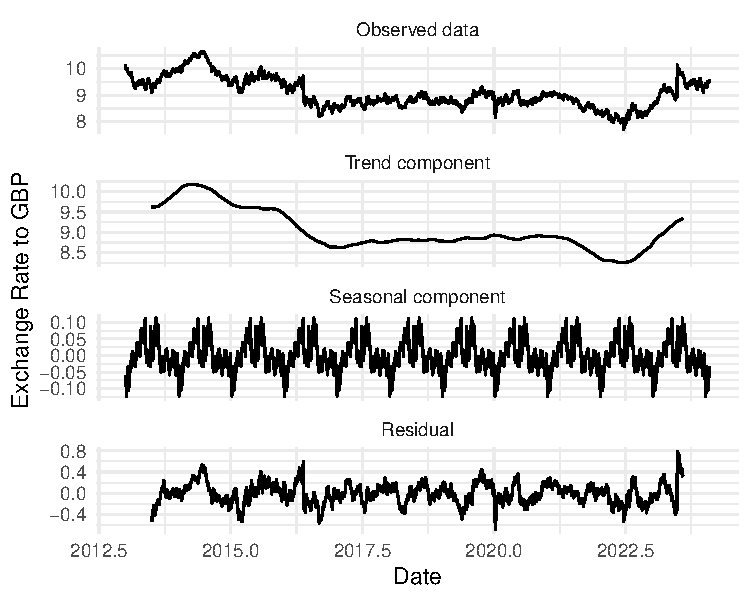
\includegraphics[width=\maxwidth]{figure/beamer-unnamed-chunk-4-1} 

}


\end{knitrout}
\centering
\caption{Decomposition of addictive time series model of CNY to GBP exchange rates}
\label{fig:decomposition of time series}
\end{figure}

\noindent
From Figure~\ref{fig:decomposition of time series}, the CNY to GBP exchange rate time series was decomposed into its fundamental components: trend, seasonality, and residual noise by additive model. This additive model, represented mathematically as $X_t = t_t + s_t + r_t$.\\

\noindent
As illustrated in Figure~\ref{fig:decomposition of time series}, the trend component $t_t$ of CNY to GBP exchange rate exhibits a distinct pattern over time: initially, it shows a gradual decrease and reached crest in 2022, followed by a sudden increase afterwards. It coincides with the tax reduction policy issued by UK government in 2022, which leads to a depreciation of GBP. This trend is pivotal for understanding the broader economic relationship between these currencies. \\

\noindent
Moreover, the seasonal component $s_t$ of the decomposition highlights cyclical fluctuations, indicative of recurrent patterns within the year. These could be attributed to seasonal economic activities, policy changes, or other cyclical factors influencing the currency market. The clear demarcation of these cyclical trends in the seasonal component helps in isolating such effects from the overarching trend.\\

\noindent
Lastly, the residual component $r_t$ encompasses the random, unexplained variations after accounting for the trend and seasonal factors. analysing these residuals is crucial for understanding the unpredictability in the exchange rate and can be pivotal in risk management and forecasting.\\

\noindent
\textbf{Autocorrelation Analysis of CNY to GBP Exchange Rate}\\
\noindent
Autocorrelation, also referred to as serial correlation, is a crucial concept in time series analysis. It describes the correlation of a time series with its own past and future values. The autocorrelation function (ACF) measures the linear predictability of the series at lag h, which is the time $t$ with its values at a previous time $t-h$. The mathematical fomulation of ACF of time series will be given in the following paragraph.\\

\noindent
Suppose we have a time series with observations denoted by \( x_1, \ldots, x_n \). Then the sample mean is given by $\bar{x} = \frac{1}{n} \sum_{t=1}^{n} x_t.$
And the sample autocovariance function at lag $h$ in days of our time series is
\[\hat{\gamma}(h) := \frac{1}{n} \sum_{t=1}^{n-|h|} (x_{t+|h|} - \bar{x})(x_t - \bar{x}), \quad -n < h < n \cite{Brockwell2016Introduction}.\]
Hence, the sample autocorrelation function at lag $h$ in days is given by
\[\hat{\rho}(h) := \frac{\hat{\gamma}(h)}{\hat{\gamma}(0)} = \frac{\sum_{t=1}^{n-|h|} (x_{t+|h|} - \bar{x})(x_t - \bar{x})}{\sum_{t=1}^{n} (x_t - \bar{x})^{2}}, \quad -n < h < n \cite{Brockwell2016Introduction}.\]
\noindent
The value of $\hat{\rho}(h)$ lies between -1 and +1. A value close to +1 indicates a strong positive correlation, while a value close to -1 indicates a strong negative correlation. A value near 0 suggests little to no linear correlation. A slow decay in the ACF plot indicates a strong relationship between past and present values, while spikes at specific lags may suggest seasonality. Autocorrelations outside the 95\% confidence interval are considered statistically significant.\\

\noindent
Next, visualise the ACF for the CNY to GBP exchange rate to understand its time-dependent structure better.

\begin{figure}[H]
\begin{knitrout}\scriptsize
\definecolor{shadecolor}{rgb}{0.969, 0.969, 0.969}\color{fgcolor}\begin{kframe}
\begin{alltt}
\hlcom{# PLOT OF THE AUTOCORRELATION FUNCTION}
\hlstd{acf_data} \hlkwb{<-} \hlkwd{acf}\hlstd{(MyData}\hlopt{$}\hlstd{CNYtoGBP,} \hlkwc{plot} \hlstd{=} \hlnum{FALSE}\hlstd{)}
\hlkwd{plot}\hlstd{(acf_data,} \hlkwc{main} \hlstd{=} \hlstr{""}\hlstd{,} \hlkwc{xlab} \hlstd{=} \hlstr{"Lag h"}\hlstd{,} \hlkwc{ylab} \hlstd{=} \hlstr{"ACF"}\hlstd{)}
\end{alltt}
\end{kframe}

{\centering 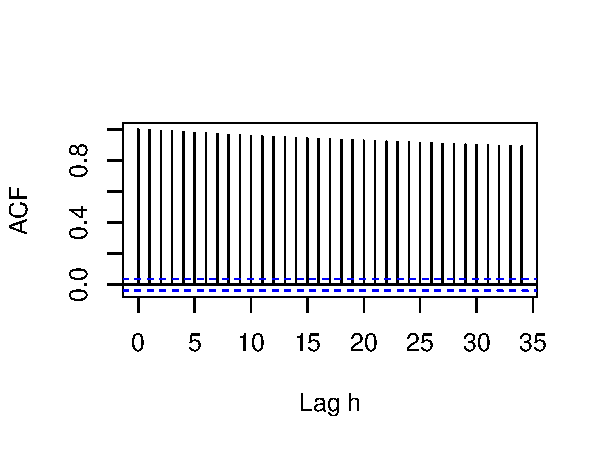
\includegraphics[width=\maxwidth]{figure/beamer-unnamed-chunk-5-1} 

}


\end{knitrout}
\centering
\caption{Autocorrelation Function at lag h in days of CNY to GBP Exchange Rate}
\label{fig:ACF}
\end{figure}

\noindent
From Figure~\ref{fig:ACF}, the ACF plot for the CNY to GBP exchange rate series reveals that the ACF starts near 1 and decreases gradually. This pattern suggests a strong persistence in the time series, indicating that past values have a significant influence on future values. In time series analysis, such a slow decay in the ACF is indicative of a non-stationary series, where the mean, variance, and autocorrelation structure do not remain constant over time.\\

\noindent
This persistent autocorrelation suggests that short-term movements in the CNY to GBP exchange rate are heavily influenced by its recent history. Such a characteristic is crucial for forecasting models, as it implies that recent historical data can be a powerful predictor of near-future trends. Models like ARIMA (Autoregressive Integrated Moving Average), which are well-suited for data with high autocorrelation, may be particularly effective in this context.

\subsection{ROC Curve}

The Receiver Operating Characteristic (ROC) anaysis is a technique for assessing the performance of classification models as its discrimination threshold is varied. Unlike univariate methods in previous subsections that are constructed from a single dataset representing one variable, ROC analysis divides a single dataset into two samples based on the actual condition of each observation, but focuses on evaluating the performance of a classification model on one variable, typically the predicted probability that a given observation belongs to a positive class. These two populations are defined as follows: the positive class (true condition positive), which includes observations that actually belong to the class of interest. The negative class (true condition negative), which includes observations that do not belong to the class of interest.\\

\noindent
\subsubsection{Theory of ROC curve}\\
Let $Y$ be a binary variable indicating the true class of an instance, with $Y = 1$ for positive instances and $Y = 0$ for negative instances. Let $X$ be a continuous variable representing the predicted score or probability of an instance being classified as positive by the classifier, with $X \geq c$ for positive and $X < c$ for negative given a threshold c.\\

\noindent
Since ROC curve plots two parameters\cite{rocAnalysis}: True Positive Rate (TPR, also known as Sensitivity, is the proportion of positive instances correctly identified) and False Positive Rate (FPR, 1 - Specificity, is the proportion of negative instances incorrectly identified as positive). Then define the TPR and the FPR using conditional probabilities as follows\cite{Pepe2003}:

\[ \text{TPR}(c) = \mathbb{P}[X \geq c | Y = 1], \quad \text{FPR}(c) = \mathbb{P}[X \geq c | Y = 0].\cite{Pepe2003}\]

\noindent
The ROC curve is then the set of points $(\text{FPR}(c), \text{TPR}(c))$ for all possible values of threshold $c$. This curve plots the trade-off between sensitivity (or TPR) and specificity (1 - FPR) across different thresholds. Let $t=\text{FPR}(c)$, then $c = \text{FPR}^{-1}(t)$ and $\text{TPR}(c)= \text{TPR}(\text{FPR}^{-1}(t))$. Hence, let $\text{ROC}(t)= \text{TPR}(\text{FPR}^{-1}(t))$, the ROC curve can be represented as a parametric function of $t$, with $t$ varying from 0 to 1:

\[ \text{ROC} = \{ (t, \text{ROC}(t)) \,|\, t \in [0, 1] \}.\cite{Pepe2003} \]

\noindent
Also, the Area Under the Curve (AUC) provides a single measure of overall performance of a classifier. This definition represents the integral of $\text{ROC}(t)$ over the interval from 0 to 1. It can be defined as:

\[ \text{AUC} = \int_{0}^{1} \text{ROC}(t) dt.\cite{Pepe2003} \]

\noindent
The larger the AUC, the better the classifier. An AUC of 0.5 suggests no discriminative ability, while an AUC of 1.0 represents perfect classification.\\

\noindent 
\subsubsection{ROC analysis in COVID-19 test}\\
The COVID-19 pandemic underscores the need for accurate diagnostic tests to differentiate between positive and negative cases\cite{Garcia2021ROCAlly}. An effective mean for evaluating accuracy of various diagnostic tests is the ROC analysis. ROC analysis comprehensively examines test accuracy by integrating TPR, FPR, and AUC. These metrics are calculated by comparing test outcomes against a recognized gold standard, thereby determining the true disease status. This approach is vital for understanding the efficacy of COVID-19 diagnostic tools and guiding public health decisions.\\

\noindent
The TPR, or sensitivity, measures the proportion of actual positives correctly identified, reflecting the test's ability to detect COVID-19 cases. The FPR, conversely, indicates the rate of false alarms, where non-infected individuals are wrongly identified as infected. An ideal test minimises FPR, avoiding unnecessary treatments or quarantine. The ROC curve visualizes the trade-off between TPR and FPR at various thresholds. A curve arching towards the upper left indicates high sensitivity and low FPR — the hallmarks of a reliable test. The AUC consolidates the ROC performance into a single value: 0.5 denotes no better accuracy than random chance, while 1.0 represents perfect accuracy. A higher AUC indicates a better overall ability of the test.\\

\noindent
Here, the simulated data will be used to demonstrate the ROC analysis in COVID-19 test. Score\_Test1 and Score\_Test2 are the simulated test scores from two different diagnostic tests for COVID-19. These scores are continuous variables that typically would represent the likelihood of a positive diagnosis. The scores might come from a lab test result, such as a PCR test or a rapid antigen test, where higher scores indicate a higher likelihood of infection. The Condition column indicates the true condition of the patient, with 1 representing a positive COVID-19 case and 0 representing a negative case.



\begin{knitrout}\scriptsize
\definecolor{shadecolor}{rgb}{0.969, 0.969, 0.969}\color{fgcolor}\begin{kframe}
\begin{alltt}
\hlcom{# PLOT OF ROC CURVES}
\hlkwd{plot}\hlstd{(roc_test1,} \hlkwc{col}\hlstd{=}\hlstr{"#459395"}\hlstd{,} \hlkwc{lwd}\hlstd{=}\hlnum{2}\hlstd{)}
\hlkwd{lines}\hlstd{(roc_test2,} \hlkwc{col}\hlstd{=}\hlstr{"#FDA638"}\hlstd{,} \hlkwc{lwd}\hlstd{=}\hlnum{2}\hlstd{,} \hlkwc{lty}\hlstd{=}\hlnum{2}\hlstd{)}
\hlkwd{legend}\hlstd{(}\hlstr{"bottomright"}\hlstd{,} \hlkwc{legend}\hlstd{=}\hlkwd{c}\hlstd{(}\hlstr{"Diagnostic Test 1"}\hlstd{,} \hlstr{"Diagnostic Test 2"}\hlstd{),}
       \hlkwc{col}\hlstd{=}\hlkwd{c}\hlstd{(}\hlstr{"#459395"}\hlstd{,} \hlstr{"#FDA638"}\hlstd{),} \hlkwc{lwd}\hlstd{=}\hlnum{2}\hlstd{,} \hlkwc{lty}\hlstd{=}\hlkwd{c}\hlstd{(}\hlnum{1}\hlstd{,} \hlnum{2}\hlstd{),} \hlkwc{cex}\hlstd{=}\hlnum{0.5}\hlstd{)}
\hlcom{# Add the perfect lines}
\hlkwd{abline}\hlstd{(}\hlkwc{h}\hlstd{=}\hlnum{1}\hlstd{,} \hlkwc{lty}\hlstd{=}\hlnum{2}\hlstd{,} \hlkwc{col}\hlstd{=}\hlstr{"red"}\hlstd{)}
\hlkwd{abline}\hlstd{(}\hlkwc{v}\hlstd{=}\hlnum{1}\hlstd{,} \hlkwc{lty}\hlstd{=}\hlnum{2}\hlstd{,} \hlkwc{col}\hlstd{=}\hlstr{"red"}\hlstd{)}
\end{alltt}
\end{kframe}\begin{figure}[H]

{\centering 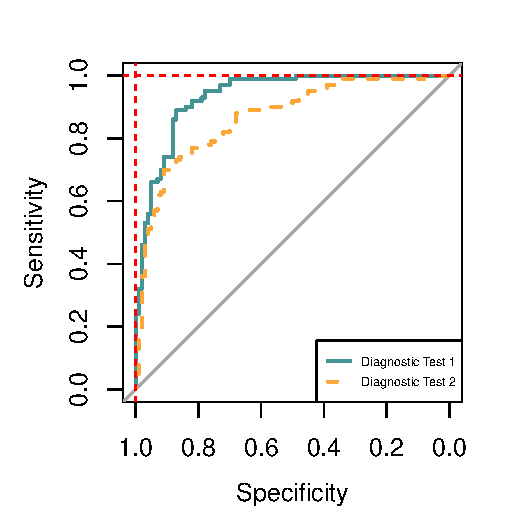
\includegraphics[width=\maxwidth]{figure/beamer-roc-1} 

}

\caption[ROC Curves for Two Diagnostic Tests]{ROC Curves for Two Diagnostic Tests}\label{fig:roc}
\end{figure}

\end{knitrout}

\noindent
From the plot~\ref{fig:roc}, the Diagnostic Test 1 has higher AUC. This test is likely to be more accurate in diagnosing COVID-19. It suggests that the test has a higher combined sensitivity and specificity, meaning it can identify positive cases more correctly and has fewer false alarms. Also, the Diagnostic Test 2 has a lower AUC than Test 1, This test is less accurate but still better than random guessing. It may miss more true cases (lower sensitivity) or incorrectly identify healthy individuals as having COVID-19 (higher false positive rate).\\

\noindent
In practice, the choice of which test to use may depend on other factors. For instance, if the cost of missing a COVID-19 case is high (for example, in a nursing home setting), a test with higher sensitivity might be preferred. Conversely, if the cost of false positives is high (for example, leading to unnecessary quarantine), a test with higher specificity might be favored.

\newpage

\section{Bivariate Data Visualisation Methods}

\noindent This chapter transitions from the study of univariate data visualisations to the exploration of bivariate data. Fundamental bivariate data visualisation methods, including heatmaps, scatter plots, and bubble charts, are introduced, scrutinised, and modelled throughout this chapter. In order to facilitate a more profound analysis of bivariate data, the chapter further delves into the examination of linear regression, as well as LOESS regression. Notably, within the context of scatter plots, an intriguing deviation is observed with the incorporation of animated data visualisations.

\subsection{Heatmaps}
The heatmap is a data visualisation technique that uses colour coding to represent different intensities. It can be represented as an $m \times n$ matrix $\mathbf{M}$, with $m$ observations for variable 1 and $n$ observations for variable 2:

$$\mathbf{M} =
\left[
\begin{array}{cccc}
    \mathrm{M}_{11} & \mathrm{M}_{12} & \ldots & \mathrm{M}_{1n} \\  
    \mathrm{M}_{21} & \mathrm{M}_{22} & \ldots & \mathrm{M}_{2n} \\  
    \vdots & \vdots & \ddots & \vdots \\  
    \mathrm{M}_{m1} & \mathrm{M}_{m2} & \ldots & \mathrm{M}_{mn}
\end{array}
\right],
$$

\noindent
where each entry $\mathrm{M}_{mn}$ represent an observation.\\

\noindent
In this illustrative example, heatmaps are used to visualise fire occurrences in Brazil. These heatmaps provide a spatially coherent representation, highlighting regions at high risk and seasonal patterns. The data-driven insights could empower policymakers to make informed decisions regarding preventive measures and firefighting strategies.\\

\noindent
In Figure~\ref{fig:fire22}, it can be observed that significantly higher fire counts are found in certain locations. The presence of two strips with high frequencies of fires are highly unusual. The vertical trend corresponds to the location of BR-230 (Trans-Amazonian Highway) passing through the city of Apuí, State of Amazonas. The horizontal trend corresponds to BR-163 (Brazil highway) passing through Três Pinheiros in Novo Progresso, State of Pará. The western coastal area with a high frequency of fire occurrence corresponds to regions in close proximity to the cities of Vista Alegre do Abunã and Rio Branco. Research has indicated that 95 \% of active fires and the most intense ones (FRP $>$ 500 megawatts) occurred at the edges in forests \cite{forest}.\\

\noindent
The seasonal pattern of fire frequency is shown in Figure~\ref{fig:fire-by-months-fy13-22}. Observe that more fire occur in the months of August to October compared to the rest of the year.









\begin{figure}[htbp]
  \centering
  \begin{minipage}[b]{0.48\linewidth}
\begin{knitrout}\scriptsize
\definecolor{shadecolor}{rgb}{0.969, 0.969, 0.969}\color{fgcolor}

{\centering 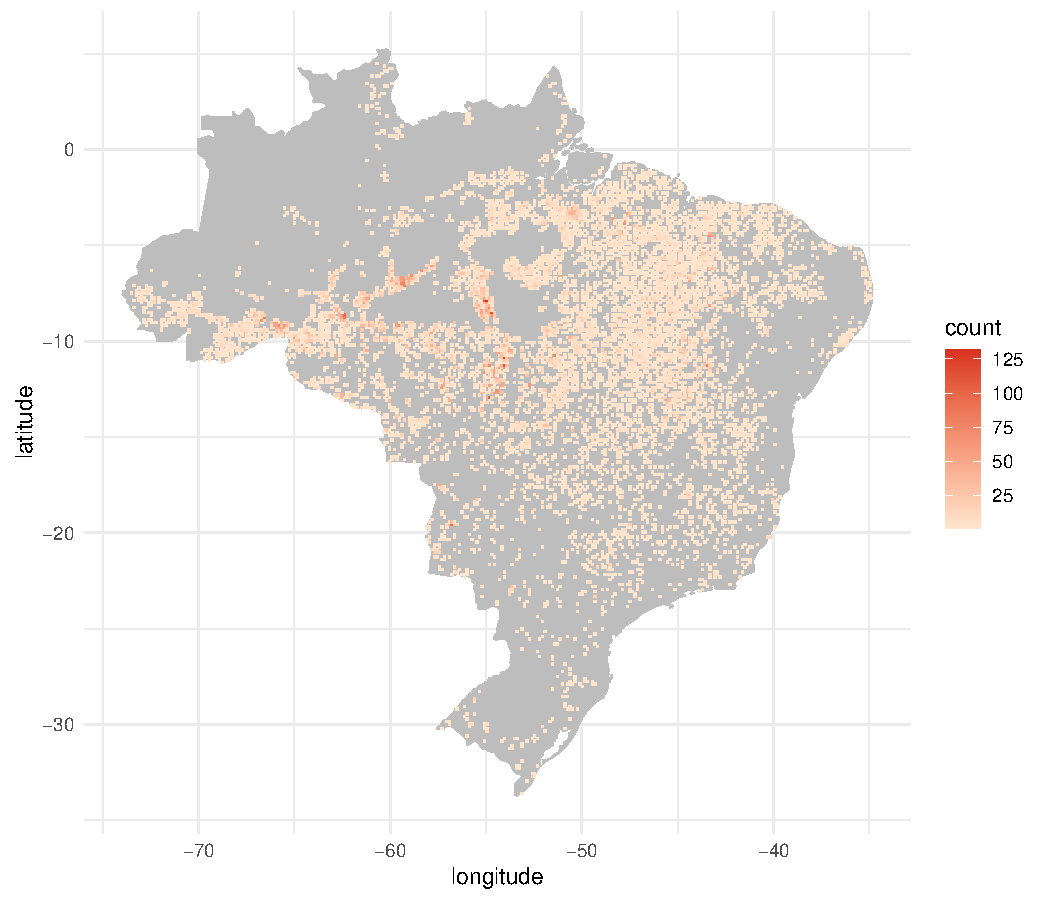
\includegraphics[width=\maxwidth]{figure/beamer-spacetime-fy22-1} 

}


\end{knitrout}
  \end{minipage}
  \hfill
  \begin{minipage}[b]{0.48\linewidth}
\begin{figure}[H]
    \centering
    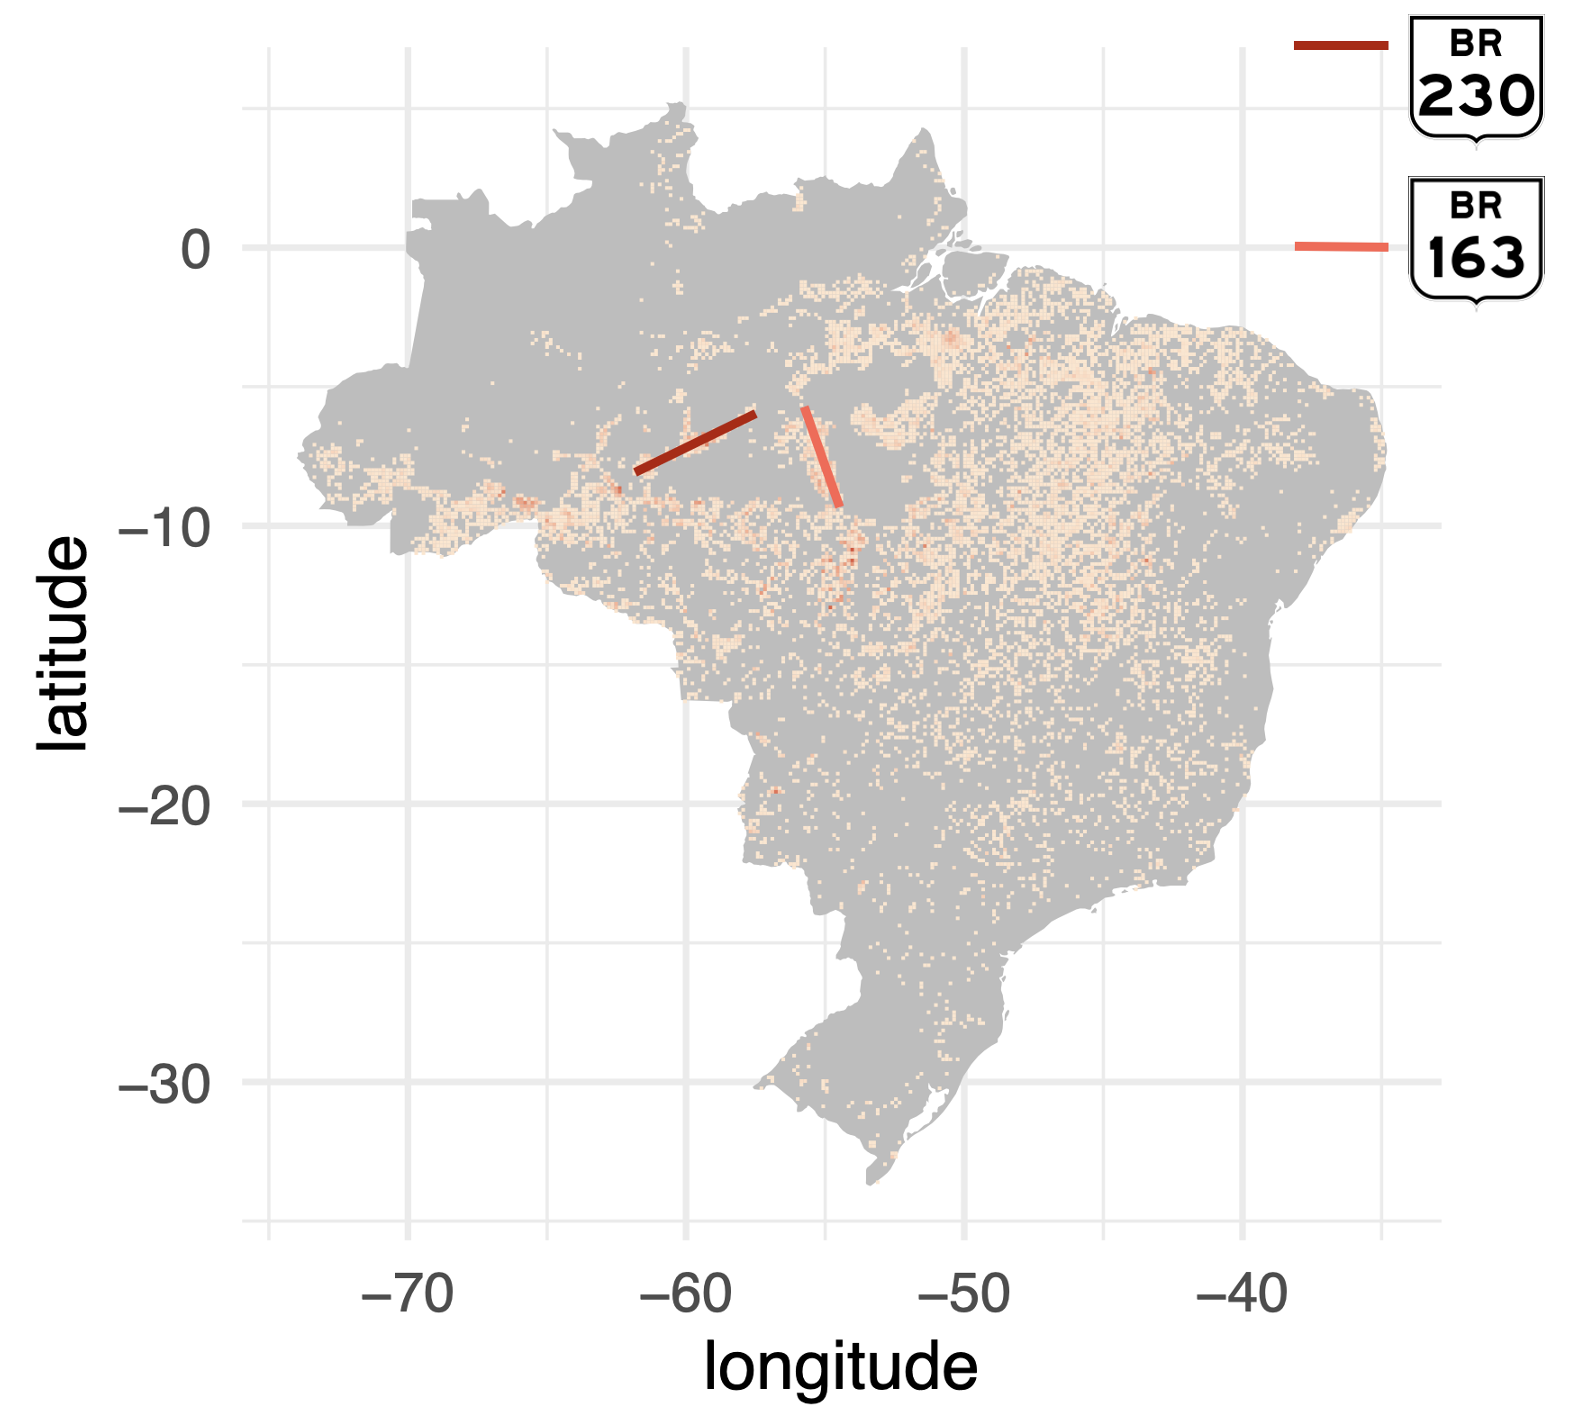
\includegraphics[width=1\linewidth]{image_reference/mapshoot.png}
\end{figure}
  \end{minipage}
  \caption{Frequency of fire in Brazil (2022), two strips of high frequencies of fires are highly unusual}
  \label{fig:fire22}
\end{figure}



\begin{knitrout}\scriptsize
\definecolor{shadecolor}{rgb}{0.969, 0.969, 0.969}\color{fgcolor}\begin{kframe}
\begin{alltt}
\hlcom{# Heatmap plot}
\hlstd{heatmap_plot} \hlkwb{<-} \hlkwd{ggplot}\hlstd{(pivot_table,}
                       \hlkwd{aes}\hlstd{(}\hlkwc{x} \hlstd{=} \hlkwd{factor}\hlstd{(abb_month,} \hlkwc{levels} \hlstd{= custom_order),}
                           \hlkwc{y} \hlstd{=} \hlkwd{as.character}\hlstd{(year),} \hlkwc{fill} \hlstd{= count))} \hlopt{+}
  \hlkwd{geom_tile}\hlstd{()} \hlopt{+}
  \hlkwd{scale_fill_gradient}\hlstd{(}\hlkwc{low} \hlstd{=} \hlstr{"#fff7ec"}\hlstd{,} \hlkwc{high} \hlstd{=} \hlstr{"#d7301f"}\hlstd{)} \hlopt{+}
  \hlkwd{labs}\hlstd{(}\hlkwc{x} \hlstd{=} \hlstr{" "}\hlstd{,} \hlkwc{y} \hlstd{=} \hlstr{" "}\hlstd{)} \hlopt{+}
  \hlkwd{theme_minimal}\hlstd{()} \hlopt{+}
  \hlkwd{theme}\hlstd{(}\hlkwc{axis.text} \hlstd{=} \hlkwd{element_text}\hlstd{(}\hlkwc{size} \hlstd{=} \hlnum{9}\hlstd{))}

\hlkwd{print}\hlstd{(heatmap_plot)}
\end{alltt}
\end{kframe}\begin{figure}[H]

{\centering 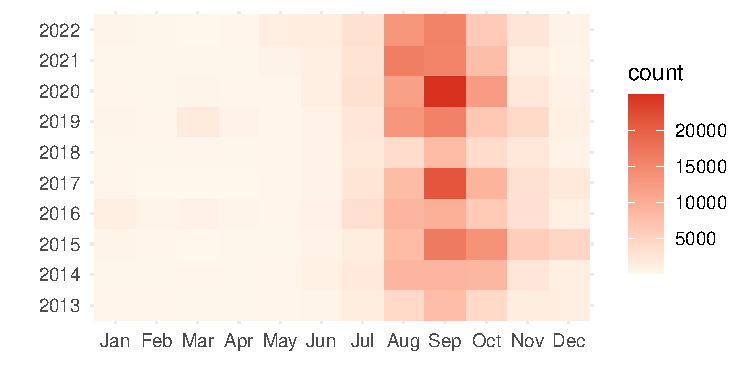
\includegraphics[width=\maxwidth]{figure/beamer-fire-by-months-fy13-22-1} 

}

\caption[Frequency of fire in Brazil (2013-2022)]{Frequency of fire in Brazil (2013-2022)}\label{fig:fire-by-months-fy13-22}
\end{figure}

\end{knitrout}


\subsection{Scatter Plots}

A scatter plot is a graphical representation of a set of data points in a two-dimensional coordinate system. Each data point is represented by a dot, and the position of the dot is determined by the values of two variables. Some examples of this type of visualisation can be found in Figures~\ref{fig:abs-plots}, ~\ref{fig:cogload-plot}, and ~\ref{fig:bubble-plot-construction}.\\

\noindent
In general, the \(Y\)-axis denotes the response, or dependent, variable and the \(X\)-axis denotes the explanatory, or independent,  variable. Each observation of a dataset is mapped to a dot in the 2-dimentional space. Let \((x_i, y_i)\) represent the coordinates of the \(i\)-th data point on the scatter plot produced by mapping a set of data. The scatter plot can be mathematically described as a set of points: \( \{(x_1, y_1), \ldots, (x_n, y_n)\}\) where \(n\) is the number of observations in the set.\\

\noindent The scatter plots in Figure~\ref{fig:bubble-plot-construction} visualise data from the mtcars dataset. Each of these three graphs represents different information drawn from the dataset. The first plot displays the various car models and their corresponding miles per gallon. The middle plot, once again, shows the car models, but this time their horsepower is represented. Finally, the last scatter plot visualises the relationship between the cars' miles per gallon and their horsepower.

\begin{knitrout}\scriptsize
\definecolor{shadecolor}{rgb}{0.969, 0.969, 0.969}\color{fgcolor}\begin{figure}[H]

{\centering 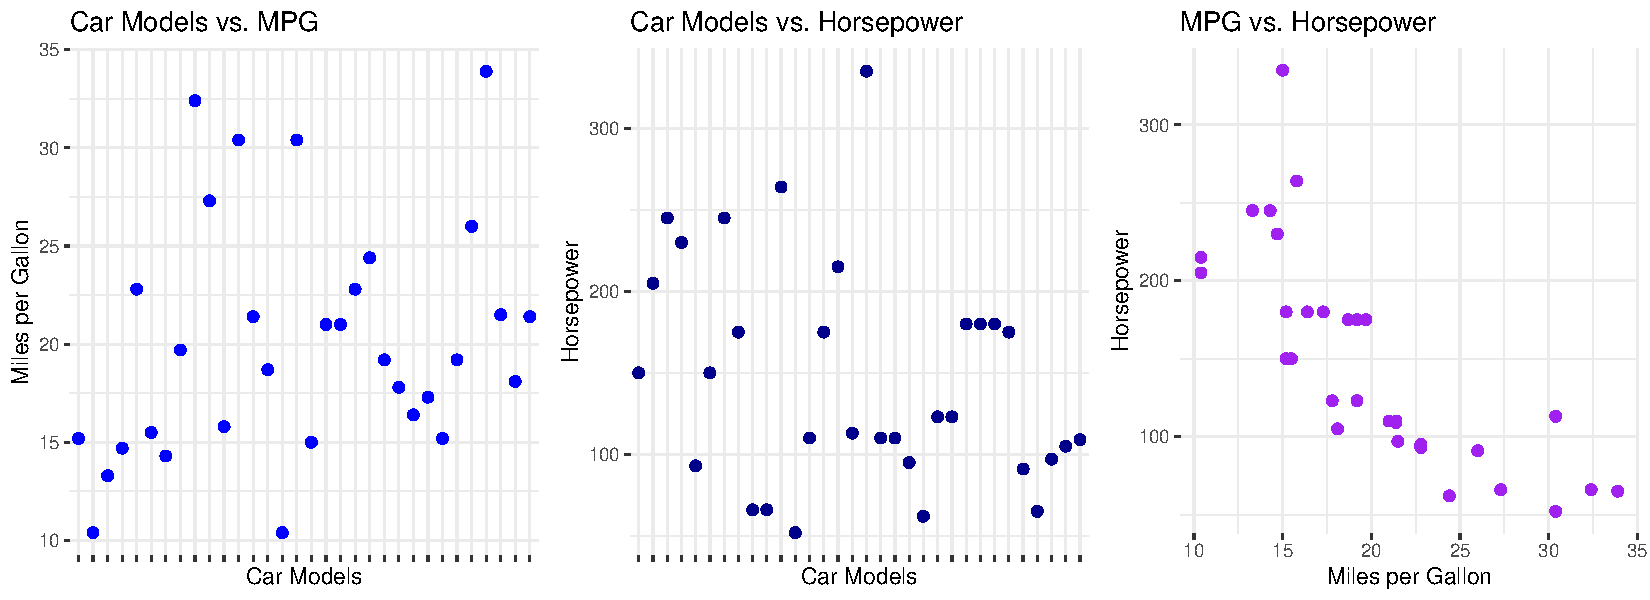
\includegraphics[width=\maxwidth]{figure/beamer-bubble-plot-construction-1} 

}

\caption[Partial scatter plot deconstruction of the mtcars dataset]{Partial scatter plot deconstruction of the mtcars dataset}\label{fig:bubble-plot-construction}
\end{figure}

\end{knitrout}

\subsubsection{Animated Scatter Plots}
\noindent While static scatter plots are effective in depicting relationships between two variables, animated scatter plot visualisations take this a step further by introducing, for example, a temporal dimension to the data visualisation. Unlike static plots, animated scatter plots enable the depiction of changes in relationships, clusters, or outliers over time. In R, the $gganimate$ package, building on the foundation of $ggplot2$ package, facilitates the creation of animated plots, including animated scatter plots. \\

\noindent
\subsubsection{\textt{gganimate} in Practice}\\
\noindent
The figure below depicts a static scatter plot illustrating the relationship between GDP per capita and life expectancy across various countries. GDP per capita is displayed on a logarithmic scale along the x-axis, and life expectancy is shown on the y-axis. The size of each point on the plot corresponds to the population size of the country it represents, and the colour of each point distinguishes one country from another.\\

\begin{knitrout}\scriptsize
\definecolor{shadecolor}{rgb}{0.969, 0.969, 0.969}\color{fgcolor}\begin{figure}[H]

{\centering 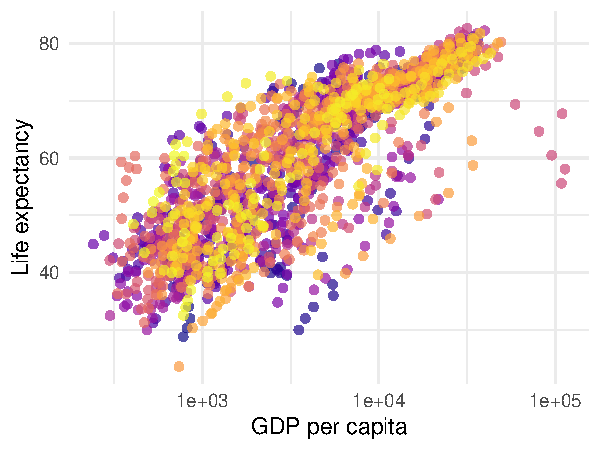
\includegraphics[width=\maxwidth]{figure/beamer-gapminder_static-1} 

}

\caption[staticl scatter plot deconstruction of the gapminder dataset]{staticl scatter plot deconstruction of the gapminder dataset}\label{fig:gapminder_static}
\end{figure}

\end{knitrout}

\noindent
In the graph we can see that there appears to be a positive correlation between GDP per capita and life expectancy, as GDP per capita increases, life expectancy also tends to be higher. \\

\noindent
However, by using the animation function, we can see how life expectancy and GDP per capita change through the years for each country, so it helps to show how relationships between variables evolve over time or across different categories. \\
\\
\begin{knitrout}\scriptsize
\definecolor{shadecolor}{rgb}{0.969, 0.969, 0.969}\color{fgcolor}\begin{kframe}
\begin{alltt}
\hlcom{# create animated ggplot}
\hlstd{gapplot}\hlkwb{<-}\hlkwd{ggplot}\hlstd{(gapminder,} \hlkwd{aes}\hlstd{(gdpPercap, lifeExp,} \hlkwc{size} \hlstd{= pop,} \hlkwc{colour} \hlstd{= country))} \hlopt{+}
  \hlkwd{geom_point}\hlstd{(}\hlkwc{alpha} \hlstd{=} \hlnum{0.7}\hlstd{,} \hlkwc{show.legend} \hlstd{=} \hlnum{FALSE}\hlstd{)} \hlopt{+}
  \hlkwd{scale_colour_manual}\hlstd{(}\hlkwc{values} \hlstd{= country_colors)} \hlopt{+}
  \hlkwd{scale_size}\hlstd{(}\hlkwc{range} \hlstd{=} \hlkwd{c}\hlstd{(}\hlnum{2}\hlstd{,} \hlnum{12}\hlstd{))} \hlopt{+}
  \hlkwd{scale_x_log10}\hlstd{()} \hlopt{+}
  \hlkwd{facet_wrap}\hlstd{(}\hlopt{~}\hlstd{continent)} \hlopt{+}
  \hlcom{# Here comes the gganimate specific bits}
  \hlkwd{labs}\hlstd{(}\hlkwc{title} \hlstd{=} \hlstr{'Year: \{frame_time\}'}\hlstd{,} \hlkwc{x} \hlstd{=} \hlstr{'GDP per capita'}\hlstd{,} \hlkwc{y} \hlstd{=} \hlstr{'life expectancy'}\hlstd{)} \hlopt{+}
  \hlkwd{transition_time}\hlstd{(year)} \hlopt{+}
  \hlkwd{ease_aes}\hlstd{(}\hlstr{'linear'}\hlstd{)}
\end{alltt}
\end{kframe}
\end{knitrout}




\subsection{Bubble Charts}
\subsubsection{Theory of Bubble Charts}
\noindent Bubble charts are a captivating data visualisation tool that extends beyond the typical two-dimensional scatter plot by introducing an extra dimension. They represent data points as bubbles or circles on a two-dimensional plane, where the size of each bubble encodes a third variable.\\

\noindent The construction of bubble charts, is parallel to that of a scatter plot, but involves the scaling the data values to determine the size of each bubble. While it isn't always the case, the size of these is typically proportional to the variable it represents. The choice of scaling method depends on the data distribution and the message the chart aims to convey.\\

\noindent Generally, the formula for calculating the bubble radius (\(R)\) involves applying the scaling function
\[
R = kV,
\]
\noindent where \(R\) represents the size of the bubble, \(V\) the value of the variable being represented, and \(k\) a scaling factor to control the bubble size. Selecting an appropriate scaling factor (\(k\)) is critical for maintaining the proportionality between the bubble size and the variable being represented.\\ 

\noindent Hence, bubble chart represents data points in three dimensions: x-coordinate, y-coordinate, and bubble size. Each data point is denoted by a triplet of values \((x_i, y_i, C_i)\), where \(x_i\) and \(y_i\) represent the coordinates, and \(C_i\) is the equation of the circle for the \(i\)-th observation. In the context of a bubble chart, the radius \(R_i\) of each bubble is expressed as \(k \cdot V_i\), allowing us to formulate the equation for each circle as:

\[
(x - x_i)^2 + (y - y_i)^2 = (kV_i)^2 ,
\]

\noindent Here, \(x_i\) and \(y_i\) denote the coordinates of the circle's center.\\

\noindent Since each bubble \(B_i\) can be defined mathematically by the triplet \((x_i, y_i, C_i)\), akin to the scatter plot, the bubble plot can be described mathematically as a set of "bubbles" \( \{B_1, \ldots, B_n\}\), where \(n\) represents the number of observations in the set.\\

\noindent
\subsubsection{Bubble Charts in Practice}\\

\noindent The bubble chart shown in Figure~\ref{fig:bubble-plot}, as the scatter plots above, visualises data from the mtcars dataset. The single graph deplics the relationship between car models and their fuel efficiency (mpg) while using the size of the bubbles to represent the car's horsepower (hp) and even colour-coding the bubbles based on the number of cylinders (cyl).\\

\begin{knitrout}\scriptsize
\definecolor{shadecolor}{rgb}{0.969, 0.969, 0.969}\color{fgcolor}\begin{figure}[H]

{\centering 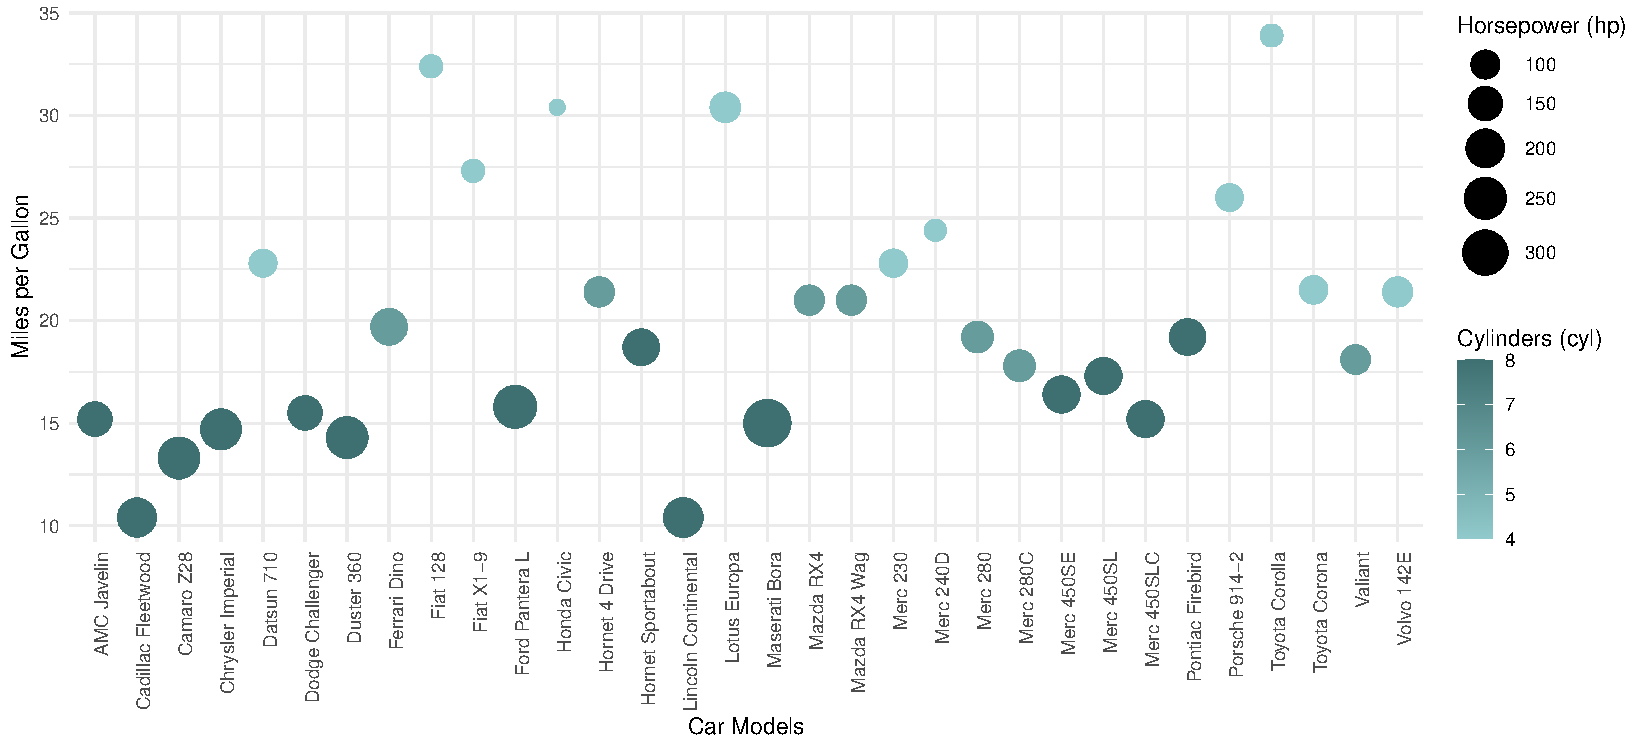
\includegraphics[width=\maxwidth]{figure/beamer-bubble-plot-1} 

}

\caption[Bubble plot illustrating trends in car types and performance]{Bubble plot illustrating trends in car types and performance}\label{fig:bubble-plot}
\end{figure}

\end{knitrout}

\\\noindent In Figure~\ref{fig:bubble-plot} a strong correlation between the cars' number of cylinder and their horsepower can be quickly identified. This is due to the fact that as size of the dots (representing horsepower) increases, their colour (representing the number of cylinders) simultaneously becomes darker. Furthermore, a correlation between the miles per gallon consumed by the different types of cars and their number of cylinders and horsepower is easily identifiable in Figure~\ref{fig:bubble-plot}. This is shown by the fact that, in the same way that the darker dots cluster towards the bottom of the graph and become lighter as they reach the top of the graph, those with a large diameter also cluster near the lower part and decrease in size as they ascend. \\ 

\noindent 
The efficiency of bubble charts is highlighted by the fact that capturing just some of the information provided by this single bubble chat - that is, the information regarding the car models, the miles covered per gallon, and the horsepower of each of these, requires three different scatter plots. These are displayed in Figure~\ref{fig:bubble-plot-construction}. The contrast between the simplicity and readability of Figure~\ref{fig:bubble-plot}, and the density and complexity of Figure~\ref{fig:bubble-plot-construction} emphasises the advantages of bubble charts in representing datasets with a higher number of variables. 


\subsection{Simple Linear Regression}
\\Regression models are statistical tools that provide functions to estimate the relationship between the response variable and one or more explanatory variables. Regression analysis is widely adopted by data scientists, who use large datasets to build predictive models for trend forecasting. The fol- lowing paragraphs will introduce simple linear regression models and demonstrate their usage using the mtcars dataset.

\subsubsection{Theory of Simple Linear Regression} 

\\Let $\mathbf{x} = (x_1, \dots, x_n)^T$ denote $n$ explanatory variables and let $\mathbf{Y} = (Y_1, \dots, Y_n)^T$ denote $n$ corresponding response variables.
\\  
\\In a simple linear model, it is assumed that the response variables $Y_1, \dots, Y_n$ are uncorrelated with a common variance $\sigma^2$, and their expectations are given by $E(Y_i| x_i) = \beta_0 + \beta_1 x_i$. The expectations generated by $\beta_0$ and $\beta_1$ given $x_i$ can be expressed as:

\begin{equation}\label{eq:4-1}
\mathrm{E}(\mathbf{Y} | \mathbf{x}) =
\left( \begin{array}{ccc}
\beta_0+\beta_1 x_1\\
\vdots\\
\beta_0+\beta_1 x_n
\end{array} \right) = 
\left( \begin{array}{ccc}
1\\
\vdots\\
1
\end{array} \right) \beta_0 + 
\left( \begin{array}{ccc}
x_1\\
\vdots\\
x_n
\end{array} \right) \beta_1 =
\mathbf{1}_n \beta_0 + \mathbf{x} \beta_1 ,
\end{equation}
\\
\noindent
where $\mathbf{1}_n$ is an n-vector of 1's.
\\  
\\Given design matrix $\mathbf{X}$ where $\mathbf{x}_i = (1, x_i)$ and $\mathbf{\beta} = (\beta_0, \beta_1)^T$, then $E(Y_i|x_i) = \mathbf{x}_i \beta$. These assumptions can be equivalently written in the vector form:

\begin{equation}\label{eq:4-2}
\mathrm{E}(\mathbf{Y} | \mathbf{x}) = 
\left( \begin{array}{cc}
1 & x_1\\
\vdots& \vdots\\
1 & x_n
\end{array} \right) 
\left( \begin{array}{cc}
\beta_0 \\
\beta_1
\end{array} \right) = \mathbf{X} \boldsymbol{\beta}, \quad 
\text{var}(\mathbf{Y} | \mathbf{x}) =
\begin{pmatrix}
\sigma^2 & 0 & \cdots & 0 \\
0 & \sigma^2 & \cdots & 0 \\
\vdots & \vdots & \ddots & \vdots \\
0 & 0 & \cdots & \sigma^2
\end{pmatrix} = \sigma^2 \mathbf{I}_n.
\end{equation}

\subsubsection{Theory of Least Squares Estimation}

\noindent The residual sum of squares (RSS) is a measure of the goodness of fit in a regression model, where residuals are the differences between the response variables $y_i$ and responses generated by the regression model $\mathrm{E}(\mathbf{Y}_i | \mathbf{x})$. In least squares estimation, the goal is to find values of parameters $\boldsymbol{\beta} = (\beta_0, \beta_1)^T$ to minimise the RSS, denoted by $\mathrm{Q}$: 

\begin{equation}\label{eq:4-3}
\mathrm{Q} = \sum_{i=1}^{n} [y_i - \mathrm{E} (Y_i | \mathbf{x})]^2 
           = [\mathbf{y}- \mathrm{E} (\mathbf{Y} | \mathbf{x})]^{T} [\mathbf{y}- \mathrm{E} (\mathbf{Y} | \mathbf{x})] 
           = (\mathbf{y}- \mathbf{X} \boldsymbol{\beta})^{T} (\mathbf{y}- \mathbf{X} \boldsymbol{\beta}),
\end{equation}

\noindent
where $\mathbf{y}$ is n-vector of response variables and $\mathbf{X}$ is the $n \times 2$ design matrix. The partial derivative of $Q$ with respect to vector $\boldsymbol{\beta}$ is:

\begin{equation}\label{eq:4-4}
\frac{\partial Q}{\partial \boldsymbol{\beta}} = 2(\mathbf{X}^T\mathbf{X} \boldsymbol{\beta} - \mathbf{X}^T\mathbf{y}),
\end{equation}

\noindent
Equating $\frac{\partial Q}{\partial \boldsymbol{\beta}} = \mathbf{0}$, the vector $\hat{\boldsymbol{\beta}}$, the least squares estimate of $\boldsymbol{\beta}$, can be written as:

\begin{equation}\label{eq:4-5}
\mathbf{X}^T(\mathbf{y}-\mathbf{X}\hat{\boldsymbol{\beta}})=\mathbf{0}.
\end{equation}

\noindent 
The least squares estimate of $\boldsymbol{\beta}$ is given by:
\begin{equation}\label{eq:4-6}
\hat{\boldsymbol{\beta}} = (\mathbf{X}^T\mathbf{X})^{-1}\mathbf{X}^T\mathbf{y}.
\end{equation}
\\ 
\noident 
\subsubsection{Case example: 1970s automobiles}\\
\noindent In this section, we will study the performance of 1970s automobiles using the mtcars dataset, employing the method of linear regression. Performance is measured in Miles per Gallon (mpg); the higher the mileage, the more efficient the automobile. We will start with the visualisation of a simple linear regression model, followed by the discussion of linear regression models and the model selection method.

\noindent
\\In the preliminary stages of data exploration, calculating the correlation matrix is a crucial step before engaging in regression modeling, as shown in Figure~\ref{fig:cor-matrix-mtcars2}. In real-world scenarios, variables are often correlated, and entirely independent relationships are seldom encountered. Therefore, analysing pairwise correlations becomes essential. This helps in understanding multicollinearity issues within the model. Multicollinearity occurs when one covariate within the model can be accurately predicted from another covariate. When this happens, the coefficient estimates of the model can change unpredictably due to minor changes in the data.\\



\begin{knitrout}\scriptsize
\definecolor{shadecolor}{rgb}{0.969, 0.969, 0.969}\color{fgcolor}\begin{figure}[H]

{\centering 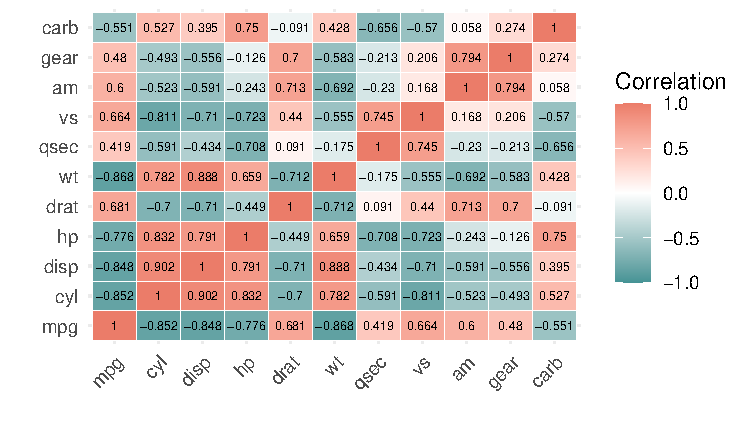
\includegraphics[width=\maxwidth]{figure/beamer-cor-matrix-mtcars2-1} 

}

\caption[Correlation matrix of all variables in mtcars dataset]{Correlation matrix of all variables in mtcars dataset}\label{fig:cor-matrix-mtcars2}
\end{figure}

\end{knitrout}

\noindent
For the simple linear regression model, the response variable is Miles per Gallon (mpg), and we select weight (wt) as the explanatory variable. Note that mpg and wt are highly correlated, with a correlation coefficient of -0.868. This suggests that wt may have strong predictive power for mpg. Use the R function \texttt{lm()} to calculate the linear regression model, with the summary displayed below.\\

\noindent
Observe that the t-test yields a p-value of $1.29 \times 10^{-10}$, which is less than $0.001$. This indicates that the variable wt holds high statistical significance in this model. For the fitted model, the slope is $\beta_1 = -5.3445$, meaning that for every increase of 1000 lbs, the car efficiency decreases by 5 miles per gallon. The RSS is 3.046. The simple linear regression line is displayed in Figure~\ref{fig:scatter-plot}.

\begin{knitrout}\scriptsize
\definecolor{shadecolor}{rgb}{0.969, 0.969, 0.969}\color{fgcolor}\begin{kframe}
\begin{alltt}
\hlcom{# Summary for simple linear regression, with response variable Miles per Gallon}
\hlstd{Modelwt} \hlkwb{<-} \hlkwd{lm}\hlstd{(}\hlkwc{formula} \hlstd{= mpg} \hlopt{~} \hlstd{wt,} \hlkwc{data} \hlstd{= mtcars)}
\hlkwd{summary}\hlstd{(Modelwt)}
\end{alltt}
\begin{verbatim}
## 
## Call:
## lm(formula = mpg ~ wt, data = mtcars)
## 
## Residuals:
##     Min      1Q  Median      3Q     Max 
## -4.5432 -2.3647 -0.1252  1.4096  6.8727 
## 
## Coefficients:
##             Estimate Std. Error t value Pr(>|t|)    
## (Intercept)  37.2851     1.8776  19.858  < 2e-16 ***
## wt           -5.3445     0.5591  -9.559 1.29e-10 ***
## ---
## Signif. codes:  0 '***' 0.001 '**' 0.01 '*' 0.05 '.' 0.1 ' ' 1
## 
## Residual standard error: 3.046 on 30 degrees of freedom
## Multiple R-squared:  0.7528,	Adjusted R-squared:  0.7446 
## F-statistic: 91.38 on 1 and 30 DF,  p-value: 1.294e-10
\end{verbatim}
\end{kframe}
\end{knitrout}

\begin{knitrout}\scriptsize
\definecolor{shadecolor}{rgb}{0.969, 0.969, 0.969}\color{fgcolor}\begin{figure}[H]

{\centering 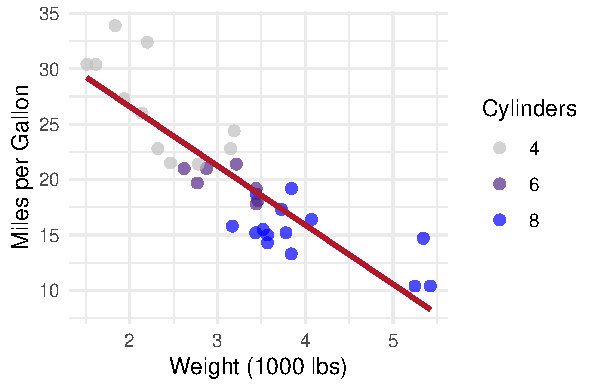
\includegraphics[width=\maxwidth]{figure/beamer-scatter-plot-1} 

}

\caption[Scatter plot of car weights vs MPG]{Scatter plot of car weights vs MPG}\label{fig:scatter-plot}
\end{figure}

\end{knitrout}

\subsection{LOESS Regression}
\noindent
Locally weighted scatterplot smoothing (LOWESS) is a local regression method for a response variable $Y$ on a single predictor $X$. LOWESS was proposed by William S. Cleveland in 1979, it is the special case to higher dimention locally estimated scatterplot smoothing (LOESS) regression method. They are non-parametric regression methods that fits a linear regression model for each neighbourhood of data. Unlike GLM, the LOESS model does not provide a global function to fit the data; rather, it fits neighborhoods of the data.\\

\noindent
\subsubsection{Theory of LOESS regression}\\

\noindent
Suppose we have $n$ ordered observations $\{(x_1,y_1), \dots, (x_n,y_n)\}$ with predictors $x_i$ and response variables $y_i$. Assume a model of the form

$$y_i = g(x_i) +  \varepsilon_i,$$
\noindent
where $\mathrm{g}$ is an unknown smooth function and $\varepsilon_i$ is i.i.d.Gaussian error terms with mean $0$ and variance $\sigma^2$.\\

\noindent
Let $\Delta_i(x) = |x - x_i|$ represent the horizontal distance between $x$ and $x_i$. Let $\Delta_{(i)}(x)$ denote the ordered distances to $x$, arranged from smallest to largest.\\

\noindent
For each point $(x,y)$ consider the neighbourhood to fit a line segment around it. The size of the neighbourhood indicates the number of data points used to fit the line segments and is determined by the smoothing parameter $\alpha$. For $\alpha \leq 1$, each  neighbourhood consists of $\frac{n}{\alpha}$ number of points \cite{rloess}. Each point $(x_i, y_i)$ in the neighbourhood of point $(x,y)$ is assigned with a weight, ``importance" of the data point to the line segment \cite{ytloess}. The weight of $(x_i,y_i)$ is denoted as $w_i(x)$, which is defined as:

\begin{equation}\label{eq:4-7}
w_i(x) = T(\Delta_i (x); \Delta _{(q)}(x)).
\end{equation}

\noindent
Tricube weight function $T(u,t)$ is defined as:
\begin{equation}\label{eq:4-8}
T(u;t) = \left\{
  \begin{array}{ll}
    (1-(u/t)^3)^3 & \text{for } 0 \leq u < t \\
    0 & \text{for } u \geq t \\
  \end{array}
\right, 
\end{equation}

\noindent
where $u$ is the horizontal distance between neighbourhood point of interest $(x_i,y_i)$ to point $(x,y)$ and $t$ is the maximum distance threshold. For points in the neighbourhood with horizontal distance exceeding threshold $t$, they are assigned with weight $0$ by the tricube weight function.\\

\noindent
For $\alpha > 1$, for each point $(x,y)$ the neighbourhood include all points. The maximum distance threshold is assumed to be $\alpha^{\frac{1}{p}}$, for $p$ explanatory variables. The weight is given by:

\begin{equation}\label{eq:4-9}
w_i(x) = T(\Delta_i (x); \Delta _{(n)}(x))\alpha.\\
\end{equation}

\noindent
The line segment is fitted by weighted least square, and this is the preliminary estimation $\hat{g}(x)$ for every point $(x,y)$.\\

\noindent
Both LOWESS and LOESS penalise the outliers in the preliminary estimation by assigning points further away from $\hat{g}(x)$ with less weight than before. The robustness weight (the adjusted weight) is given by:
$$r_i = B(\hat{\varepsilon}_i, 6\mathrm{m}),$$

\noindent
where bisquare weight function is defined as:

\begin{equation}\label{eq:4-10}
B(u;b) = \left\{
  \begin{array}{ll}
    (1-(u/b)^2)^2 & \text{for } 0 \leq |u| < b \\
    0 & \text{for } |u| \geq b \\
  \end{array},
\right
\end{equation}

\noindent
and the median absolute residual $\mathrm{m}$ is defined as $\mathrm{m} = \mathrm{median}(|\hat{\varepsilon}_i|)$, the residual $\hat{\varepsilon}_i$ is defined as $\hat{\varepsilon}_i = y_i - \hat{y}(x_i)$. \\

\noindent
Note the process of weight adjustment using previous estimation is iterated several times until a smooth curve is obtained.\\

\noindent
The updated model estimate $\hat{g}(x)$, is computed using the local fitting method, but with the neighborhood weights $w_i{(x)$ replaced by $r_i w_i(x)$ \cite{loess}.\\

\noindent
\subsubsection{Case example: Taiwan Housing dataset}\\

\noindent
Property valuation can be modelled as a regression problem, in this analysis, we delve into the pricing of properties based on their age. Using the Taipei Housing dataset, we investigate the relationship between the age of houses (measured in years) and their prices (measured in New Taiwan dollars per unit area). Linear regression model and the LOESS regression model are used, as shown in Figure~\ref{fig:estate-data-plot}.\\

\noindent
The linear model has a residual standard error of 13.32, while the LOESS model has a residual standard error of 12.16. Cross-validation is a method to compare model goodness of fit. LOESS, with its ability to capture local variations may outperform linear regression, which minimises the least squares estimate $\hat{\beta}$.\\



\begin{knitrout}\scriptsize
\definecolor{shadecolor}{rgb}{0.969, 0.969, 0.969}\color{fgcolor}\begin{kframe}
\begin{alltt}
\hlcom{# linear regression vs. LOESS model}
\hlkwd{ggplot}\hlstd{(}\hlkwc{data} \hlstd{= estate,} \hlkwd{aes}\hlstd{(}\hlkwc{x} \hlstd{= house_age,} \hlkwc{y} \hlstd{= price_per_area))} \hlopt{+}
  \hlkwd{geom_point}\hlstd{(}\hlkwc{size} \hlstd{=}\hlnum{0.5}\hlstd{)} \hlopt{+}
  \hlkwd{theme_minimal}\hlstd{()}\hlopt{+}
  \hlkwd{scale_x_continuous}\hlstd{(}\hlkwc{labels} \hlstd{= scales}\hlopt{::}\hlkwd{number_format}\hlstd{(}\hlkwc{scale} \hlstd{=} \hlnum{1}\hlstd{))} \hlopt{+}
  \hlkwd{scale_y_continuous}\hlstd{(}\hlkwc{labels} \hlstd{= scales}\hlopt{::}\hlkwd{number_format}\hlstd{(}\hlkwc{scale} \hlstd{=} \hlnum{1}\hlstd{))} \hlopt{+}
  \hlkwd{geom_smooth}\hlstd{(}\hlkwc{method} \hlstd{=} \hlstr{"loess"}\hlstd{,} \hlkwc{se} \hlstd{=} \hlnum{FALSE}\hlstd{,} \hlkwc{color} \hlstd{=} \hlstr{"#EB7C69"}\hlstd{,} \hlkwc{span} \hlstd{=} \hlnum{0.5}\hlstd{)} \hlopt{+}
  \hlkwd{geom_smooth}\hlstd{(}\hlkwc{method} \hlstd{=} \hlstr{"lm"}\hlstd{,} \hlkwc{se} \hlstd{=} \hlnum{FALSE}\hlstd{,} \hlkwc{color} \hlstd{=} \hlstr{"#459395"}\hlstd{,} \hlkwc{formula} \hlstd{= y} \hlopt{~} \hlstd{x)} \hlopt{+}
  \hlkwd{labs}\hlstd{(}\hlkwc{title} \hlstd{=} \hlstr{"House Age vs. House Price"}\hlstd{,}
       \hlkwc{x} \hlstd{=} \hlstr{"house age (year)"}\hlstd{,}
       \hlkwc{y} \hlstd{=} \hlstr{"price (unit area)"}\hlstd{)} \hlopt{+}
  \hlkwd{theme_minimal}\hlstd{()}
\end{alltt}
\end{kframe}\begin{figure}[H]

{\centering 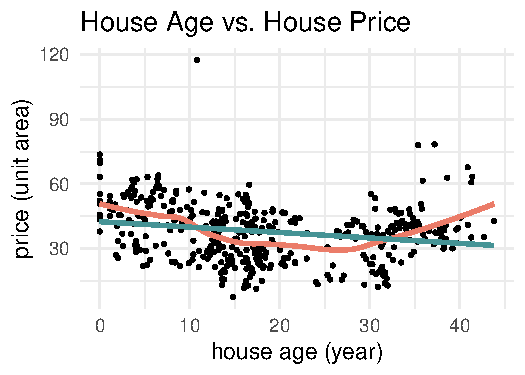
\includegraphics[width=\maxwidth]{figure/beamer-estate-data-plot-1} 

}

\caption[Estate valuation using house age, linear regression and smooth regression methods]{Estate valuation using house age, linear regression and smooth regression methods}\label{fig:estate-data-plot}
\end{figure}

\end{knitrout}

\newpage

\section{Visualising Beyond Two Dimensions}


\noindent This  chapter extends beyond the realm of two dimensional data visualisations. Within this chapter, advanced techniques are explored to unravel complex relationships involving multiple variables. The Principal Component Analysis (PCA) is introduced as a powerful method for dimensionality reduction, enabling a concise representation of high-dimensional datasets. Multiple innovative approaches facilitating the visualisation of high-dimensional data in lower-dimensional biplots and t-distributed Stochastic Neighbor Embedding (t-SNE) are studied. 

\subsection{Principal Component Analysis (PCA)}

\subsubsection{Theory of PCA}
\noindent
Principal Component Analysis (PCA) is one of the most widely-used dimensionality reduction techniques. The basic idea behind PCA is to project high-dimensional data into a low-dimensional subspace, aiming to create a visual representation that captures most of the variability present in the data.\\

\noindent
The feature matrix $\mathbf{X}$ is an $N \times D$ real-valued matrix collecting the observed data:
$$\mathbf{X} = \left( \begin{array}{ccc}
    \mathbf{x}^{T}_{1}\\
    \vdots\\
    \mathbf{x}^{T}_{n}
    \end{array} \right) = \begin{pmatrix}
x_{1,1} & x_{1,2} & \cdots & x_{1,D} \\
 &\vdots & & \\
x_{N,1} & x_{N,2} & \cdots & x_{N,D}
\end{pmatrix},$$
\noindent
with $N$ observations and $D$ variables (also known as features).\\

\noindent
Define a linear and orthogonal mapping, denoted as $\mathbf{W}: \mathbf{x} \to \mathbf{z}$ which acts as a `transformer' between high-dimensional data point $\mathbf{x}$ and its low-dimensional projection $\mathbf{z}$. Matrix $\mathbf{W}$ is defined as a $D \times L$ orthogonal and normalised matrix. Therefore, it can be expressed as column vectors $\mathbf{W} = [\mathbf{w}_1, \dots, \mathbf{w}_L]$, where $\mathbf{w}_i \mathbf{w}_j = 0$ for all $i \ne j$ and $\mathbf{w}_i^T \mathbf{w}_i = 1$. This matrix allows us to project the data from its original high-dimensional space to the low-dimensional subspace using $\mathbf{z} = \mathbf{W}^T\mathbf{x}$; this process is called encoding. To unproject $\mathbf{z}$ and obtain a high-dimensional approximation, denoted as $\hat{\mathbf{x}} = \mathbf{W}\mathbf{z}$, this process is called decoding.\\

\noindent
The optimal solution of PCA is obtained by minimising the reconstruction error subject to constraint $\mathbf{W}$, which is defined below:
$$\mathcal{L}(\mathbf{W}) = \frac{1}{N}\sum_{n=1}^{N}||\mathbf{x}_n - \hat{\mathbf{x}}||^2_2.
$$

\subsubsection{Derivation of PCA}

In general, the vector $\mathbf{w}_i$ is given by the equation $\mathbf{\Sigma} \mathbf{w}_i = \lambda \mathbf{w}_i$, where $\mathbf{\Sigma}$ is the covariance matrix and $\lambda$ is the $i^{th}$ largest eigenvalue of $\mathbf{\Sigma}$, for $i = 1, \dots, L$.\\

\noindent
Define the covariance matrix $\mathbf{\Sigma}$ as $\mathbf{\Sigma} = \frac{1}{N} \sum_{n=1}^N(\mathbf{x}_n-\bar{x})(\mathbf{x}_n-\bar{x})^T$. Without loss of generality, let's assume that the data matrix $\mathbf{X}$ is centred around $0$ mean denoted as $\bar{x} = 0$. Then, the covariance matrix can be written as:

\begin{equation}
\mathbf{\Sigma} = \frac{1}{N} \sum_{n=1}^N\mathbf{x}_n\mathbf{x}_n^T = \frac{1}{N} \mathbf{X}\mathbf{X}^T. \label{eq:cov}
\end{equation}

\noindent
The optimal encoding $\mathbf{Z}$ ensures the least amount of information loss when data is projected from a high-dimensional space to a lower-dimensional one. To determine this optimal encoding, we minimise the reconstruction error with respect to $\mathbf{w}$ and $\mathbf{z}$.

\begin{equation}
\begin{aligned}
\mathcal{L}(\mathbf{w},\mathbf{z}) &= \frac{1}{N}\sum ||\mathbf{x}_n - \mathbf{W}\mathbf{z}_n||^2  \\
&= \frac{1}{N}\sum (\mathbf{x}_n - \mathbf{W}\mathbf{z}_n)^T(\mathbf{x}_n - \mathbf{W}\mathbf{z}_n)  \\
&= \frac{1}{N}\sum \mathbf{x}_n^T\mathbf{x}_n - 2\mathbf{x}_n^T\mathbf{W}\mathbf{z}_n+\mathbf{z}_n^T\mathbf{W}^T\mathbf{W}\mathbf{z}_n . \label{eq:lossfunc}
\end{aligned}
\end{equation}

\noindent
To determine the optimal encoding $\mathbf{z}_n$ for the $n^{th}$ observation, we set the derivative with respect to $\mathbf{z}_n $ equal to $0$:

$$\frac{\partial \mathcal{L}(\mathbf{w},\mathbf{z})}{\partial \mathbf{z}_n} = \frac{1}{N} (-2 \mathbf{x}_n^T\mathbf{W} + 2\mathbf{z}_n)= \mathbf{0}.$$

\noindent
Thus we find that $\mathbf{z}_n = \mathbf{W}^T\mathbf{x}_n$ yields the optimal encoding for the $n^{th}$ observation.\\

\noindent
Next, we aim to find the matrix $\mathbf{W}$ which gives the optimal encoding. We start by expanding and simplifying the loss function $\mathcal{L}(\mathbf{W})$ from equation \ref{eq:lossfunc}: \\

\begin{equation}
\mathcal{L}(\mathbf{W}) = \frac{1}{N} \sum_{n=1}^{W}\mathbf{x}_n^T\mathbf{x}_n - \sum_{n=1}^{L}\mathbf{W}_l^T(\frac{1}{N} \sum_{n=1}^{N}\mathbf{x}_n\mathbf{x}_n^T)\mathbf{W}_l.
\end{equation}

\noindent
WLOG, our data is assumed to be centred around $0$ mean (by \ref{eq:cov}), the loss function can be represented as:

\begin{equation}
\mathcal{L}(\mathbf{W}) = \mathrm{constant} - \sum_{l=1}^L\mathbf{W}_l^T\mathbf{\Sigma}\mathbf{W}_l.
\end{equation}

\noindent 
Since $\mathbf{W}$ is a normalised matrix, it has the property $\mathbf{W}_i^T\mathbf{W}_i =1$ for all $i =1, \dots, N$. Therefore, when computing the partial derivative of $\mathcal{L}(\mathbf{W})$ with respect to vector $\mathbf{w}_1$, we can apply the Lagrange multipliers to $\mathcal{L}(\mathbf{w}_1)$ and calculate the derivative of $\hat{\mathcal{L}}(\mathbf{w}_1)$ instead:

\begin{equation}
\hat{\mathcal{L}}(\mathbf{w}_1) = - \mathbf{w}_1^T\mathbf{\Sigma}\mathbf{w}_1 + \lambda(\mathbf{w}_1^T\mathbf{w}_1 -1),
\end{equation}

\noindent 
Equating $\frac{\partial \hat{\mathcal{L}}(\mathbf{w}_1))}{\partial \mathbf{w}_1} = \mathbf{0}$, the weight vector $\mathbf{w}_1$ which minimise the loss function can be expressed as:

\begin{equation}
\frac{\partial \hat{\mathcal{L}}(\mathbf{w}_1))}{\partial \mathbf{w}_1} = 2\mathbf{\Sigma}\mathbf{w}_1+2\lambda \mathbf{w}_1 = \mathbf{0}.
\end{equation}

\noindent 
Therefore $\mathbf{\Sigma}\mathbf{w}_1 = \lambda \mathbf{w}_1$ that is, $\mathbf{w}_1$ is the eigenvector of $\mathbf{\Sigma}$ with eigenvalue $\lambda$.\\

\noindent 
Premultiply by $\mathbf{w}_1^T$, $\mathbf{w}_1^T\mathbf{\Sigma}\mathbf{w}_1 = \lambda \mathbf{w}_1^T\mathbf{w}_1 = \lambda$. To minimise the loss $\mathcal{L}}(\mathbf{w}_1)$ we maximise $\mathbf{w}_1^T\mathbf{\Sigma}\mathbf{w}_1$. Thus the largest eigenvalue $\lambda$ would minimise the loss $\mathcal{L}}(\mathbf{w}_1)$.\\

\noindent 
Adopting the same methodology, the second largest eigenvalue $\lambda$_2$ would minimise the loss $\mathcal{L}}(\mathbf{w}_2)$.\\

\noindent 
Therefore, order the eigenvectors by their corresponding eigenvalues $\{\mathbf{w}_1, \dots, \mathbf{w}_L\}$. These form the columns of the weight matrix $\mathbf{W} \in \mathbb{R}^{D \times L}$.\\

\subsection{Biplots}
\noindent 
A biplot is a graphical representation that succinctly captures the relationships between variables and observations in a reduced-dimensional space defined by the principal components. This visualisation method facilitates the exploration of complex multivariate data by providing a simultaneous display of both samples (observations) and variables in a single plot. They are commonly understood to be a generalisation of the simple two-variable scatterplot.\\

\noindent At their core, biplots offer a graphical representation of a standardised data matrix, whose rows \(n\) are the samples, and whose columns \(p\) are the variables, by projecting these onto a two-dimensional plane. To do this, mathematical computations derived from techniques like Singular Value Decomposition (SVD) and Principal Component Analysis (PCA) are required.\\

\noindent In recent years, there have been substantial developments in biplots (REFRENCE Gower and Hand in 1996). The technique has expanded far beyond what is now referred to as the "classical biplots" or "PCA biplots". The concept now finds broad application in conjunction with various other techniques of multivariate analysis. Nevertheless, this section studies the foundations of this visualisation technique, and thus, the emphasis is on biplots within the framework of PCA.

\subsubsection{Construction of PCA Biplots}

\noindent \textbf{Singular Value Decomposition}\\
\noindent Principal component biplots are based on singular value decomposition of the $(n \times p)$ data matrix $\mathbf{X}$ of $n$ observations on $p$ variables with rank $r$. The singular value decomposition of the standardised matrix $\mathbf{X}$ is found to be the following:

\[\mathbf{X} = \mathbf{U}\mathbf{B}\mathbf{S}^{T}, \]

\noindent where $\mathbf{U}$ is an $(n \times r)$ orthogonal matrix, and $\mathbf{S}$ is an $(p \times r)$ orthogonal matrix. The columns of $\mathbf{U}$ and $\mathbf{S}$ are the left and right singular vectors. $\mathbf{B}$ is a $(r \times r)$ diagonal matrix with entries $b_1, \ldots, b_r$ such that $b_1 \geq \dots b_r \geq 0$. These entries the singular values discussed later on. %Reference Miguel lecture\\

\noindent In order to find this singular value decomposition, firstly we require the computation of the orthogonal diagonalisation  

\[
\mathbf{X}^T\mathbf{X}=\mathbf{PDP}^T,
\] 

\noindent where $\mathbf{D}$ is the diagonal matrix of eigenvalues of $\mathbf{X}^T\mathbf{X}$ and $\mathbf{P}$ is an orthogonal matrix composed of the normalised eigenvectors of $\mathbf{X}^T\mathbf{X}$.\\

\noindent Now, $\mathbf{B}$ and $\mathbf{S}$ are computed. Matrix $\mathbf{S}$ is equivalent to the matrix $\mathbf{P}$ previously computed, and matrix $\mathbf{B}$ is a $(n \times p)$ diagonal matrix, where the diagonal entries are the "singular values" with any additional rows and columns of zero to make the dimensions of $\mathbf{B}$ match those of $\mathbf{X}$. The singular values referenced are square root of the eigenvalues of $\mathbf{X}^T\mathbf{X}$.Hence matrix $\mathbf{B}$ is of the form

\[
\mathbf{B} = 
\begin{bmatrix}
    \mathbf{D} & \mathbf{0} \\
    \mathbf{0} & \mathbf{0} \\
\end{bmatrix}.
\]

\noindent Finally, the $\mathbf{U}$ orthogonal matrix is calculated. The $i$-th column of $\mathbf{U}$ is given by

\[
\mathbf{u}_i = \frac{1}{\sigma_1}\mathbf{X}\mathbf{s}_i,
\]

\noindent where $\sigma_i$ are the singular values, and $\mathbf{s}_i$ are the columns of the matrix $\mathbf{S}$.\\

%Reference: https://www.youtube.com/watch?v=vbGw7BTWYS4

\noindent \textbf{PCA Biplot Construction}\\
\noindent Now, the heuristic argument motivating PCA biplots is the following. Define $\mathbf{B}^{\alpha}$, for $0 \leq \alpha \leq 1$, as a diagonal matrix who's elements are $b_1^{\alpha}, \ldots, b_r^{\alpha}$, with a similar definition for $\mathbf{B}^{1-\alpha}.$ Then, with the decomposition of matrix $\mathbf{X}$ found through SVD, the data can be further rewritten as
\[\mathbf{X} = \mathbf{U}\mathbf{B}^{\alpha}\mathbf{B}^{1-\alpha}\mathbf{S}^{T} = \mathbf{U}\mathbf{B}\mathbf{S}^{T} = \mathbf{G}\mathbf{H}^{T},\]

\noindent where \[\mathbf{G} = [\mathbf{g}_1, \dots , \mathbf{g}_n] = \mathbf{U}\mathbf{B}^\alpha, \quad \mathbf{H}^T = [\mathbf{h}_1, \dots , \mathbf{h}_p]^T = \mathbf{B}^{1-\alpha}\mathbf{S}^T. \]

\noindent Hence, the $i$th observation of the $j$th variable can be rewritten as

\[ x_{ij} = \mathbf{g}_i^T \mathbf{h}_j. \]

\noindent Both the $\mathbf{g}_i$ and $\mathbf{h}_j$ have $r$ elements, and hence, if $\mathbf{X}$ has rank 2, all could be plotted as points in two-dimensional space. Note that for the more general case, where $r > 2$, $x_{ij}$ can be written as

\[
x_{ij} = \sum_{k=1}^{r} u_{ik}b_{k}s_{jk}
\]

\noindent which is often well approximated by

\[
_m\tilde{x}_{ij} = \sum_{k=1}^{m} u_{ik}b_{k}s_{jk}, \quad \text{with } m < r.
\]

\noindent But this can be written
\[
_m\tilde{x}_{ij} = \sum_{k=1}^{m} \mathbf{g}_{ik}\mathbf{h}_{jk} = \mathbf{g}_{i}^{*T}\mathbf{h}_{j}^{*},
\]

\noindent where $\mathbf{g}^*_{i}, \mathbf{h}^*_{j}$ contain the first $m$ elements of $\mathbf{g}_i$ and $\mathbf{h}_j$ respectively. Hence, suggesting that if instead of using the $\mathbf{g}_i$ and the $\mathbf{h}_j$, we can just use their first elements (say, 2), respectively denoted by  $\mathbf{g}_{i}^{*}$  and  $\mathbf{h}_{j}^{*}$, to get

\[ x_{ij} \approx \mathbf{g}_{i}^{*T}\mathbf{h}_{j}^{*}.\]

\noindent Thus, $\mathbf{g}_i$ and $\mathbf{h}_j$ should provide a reasonable two-dimensional approximation of the $n$ observations and the $p$ variables.\\

\subsubsection{Biplots in Practice: The mtcars Dataset}

\noindent This section presents a comparative analysis of PCA biplots generated through two distinct methodologies: manual mathematical construction and use of R's in-built functions. The focus lies on elucidating the mathematical intricacies, exploring relations, and highlighting differences between the two approaches. The mtcars dataset will serve as a benchmark.\\

\noindent \textbf{Methodologies Discussion}\\
\noindent Traditionally, biplots are constructed manually through mathematical operations based on SVD discussed previously. However, with computational tools like R, in-built functions such as \texttt{prcomp()} and \texttt{biplot()} streamline the process, removing tidious mathematical intricacies, which becomes particularly interesting when working with larger datasets.\\

\noindent The manual construction, which results in the biplot shown in Figure~\ref{fig:PCAbiplot-deconstruction}, begins with data standardisation followed by SVD decomposition to obtain matrices representing row and column contributions to principal components. These matrices are then utilised to construct the biplot. Conversely, the in-built function approach employs R's \texttt{prcomp()} function for PCA and directly generates the biplot using \texttt{biplot()}, without the need for explicit mathematical operations. The product of this method is shown in Figure~\ref{fig:PCAbiplot}.

\begin{knitrout}\scriptsize
\definecolor{shadecolor}{rgb}{0.969, 0.969, 0.969}\color{fgcolor}\begin{kframe}
\begin{alltt}
\hlcom{#MANUAL CONSTRUCTION OF A BIPLOT IN R}
\hlcom{# Standardise the data}
\hlstd{scaled_data} \hlkwb{<-} \hlkwd{scale}\hlstd{(mtcars)}

\hlcom{# Set the alpha parameter for SVD}
\hlstd{alpha} \hlkwb{<-} \hlnum{0}

\hlcom{# Preprocess the data using SVD}
\hlstd{preprocess} \hlkwb{<-} \hlstd{scaled_data} \hlopt{-} \hlkwd{matrix}\hlstd{(}\hlkwd{colMeans}\hlstd{(scaled_data),} \hlkwc{nrow} \hlstd{=} \hlkwd{nrow}\hlstd{(scaled_data),} \hlkwc{ncol} \hlstd{=} \hlkwd{ncol}\hlstd{(scaled_data),} \hlkwc{byrow} \hlstd{=} \hlnum{TRUE}\hlstd{)}
\hlstd{svd_mtcars} \hlkwb{<-} \hlkwd{svd}\hlstd{(preprocess)}
\hlstd{U} \hlkwb{<-} \hlstd{svd_mtcars}\hlopt{$}\hlstd{u}
\hlstd{L} \hlkwb{<-} \hlkwd{diag}\hlstd{(svd_mtcars}\hlopt{$}\hlstd{d)}
\hlstd{A} \hlkwb{<-} \hlstd{svd_mtcars}\hlopt{$}\hlstd{v}

\hlcom{# Calculate G and H matrices}
\hlstd{G} \hlkwb{<-} \hlstd{U} \hlopt \hlstd{(L}\hlopt\hlstd{(alpha))}
\hlstd{H} \hlkwb{<-} \hlkwd{t}\hlstd{((L}\hlopt \hlstd{(}\hlnum{1}\hlopt{-}\hlstd{alpha))} \hlopt \hlkwd{t}\hlstd{(A))}

\hlcom{# Extract the first two columns for biplot}
\hlstd{G2} \hlkwb{<-} \hlstd{G[,} \hlnum{1}\hlopt{:}\hlnum{2}\hlstd{]}
\hlstd{H2} \hlkwb{<-} \hlstd{H[,} \hlnum{1}\hlopt{:}\hlnum{2}\hlstd{]}

\hlcom{# Create a biplot-like plot}
\hlkwd{par}\hlstd{(}\hlkwc{mfrow} \hlstd{=} \hlkwd{c}\hlstd{(}\hlnum{1}\hlstd{,} \hlnum{2}\hlstd{),} \hlkwc{pty} \hlstd{=} \hlstr{"s"}\hlstd{)}
\hlkwd{plot}\hlstd{(G2,} \hlkwc{xlim} \hlstd{=} \hlkwd{c}\hlstd{(}\hlopt{-}\hlnum{0.25}\hlstd{,} \hlnum{0.4}\hlstd{),} \hlkwc{xlab} \hlstd{=} \hlstr{"PC1"}\hlstd{,} \hlkwc{ylab} \hlstd{=} \hlstr{"PC2"}\hlstd{)}
\hlkwd{par}\hlstd{(}\hlkwc{new} \hlstd{=} \hlnum{TRUE}\hlstd{)}
\hlkwd{plot}\hlstd{(H2,} \hlkwc{xlim} \hlstd{=} \hlkwd{c}\hlstd{(}\hlopt{-}\hlnum{4.5}\hlstd{,} \hlnum{8}\hlstd{),} \hlkwc{ylim} \hlstd{=} \hlkwd{c}\hlstd{(}\hlopt{-}\hlnum{4.5}\hlstd{,} \hlnum{8}\hlstd{),} \hlkwc{col} \hlstd{=} \hlstr{"#EB7C69"}\hlstd{,}
     \hlkwc{xaxt} \hlstd{=} \hlstr{"n"}\hlstd{,} \hlkwc{yaxt} \hlstd{=} \hlstr{"n"}\hlstd{,} \hlkwc{xlab} \hlstd{=} \hlstr{""}\hlstd{,} \hlkwc{ylab} \hlstd{=} \hlstr{""}\hlstd{)}

\hlcom{# Draw pseudo-axis}
\hlkwa{for} \hlstd{(i} \hlkwa{in} \hlnum{1}\hlopt{:}\hlkwd{ncol}\hlstd{(scaled_data)) \{}
  \hlkwd{lines}\hlstd{(}\hlkwd{c}\hlstd{(}\hlnum{0}\hlstd{, H2[i,} \hlnum{1}\hlstd{]),} \hlkwd{c}\hlstd{(}\hlnum{0}\hlstd{, H2[i,} \hlnum{2}\hlstd{]),} \hlkwc{col} \hlstd{=} \hlstr{"#EB7C69"}\hlstd{,} \hlkwc{lwd} \hlstd{=} \hlnum{1.5}\hlstd{)}
\hlstd{\}}

\hlkwd{axis}\hlstd{(}\hlnum{3}\hlstd{)}
\hlkwd{axis}\hlstd{(}\hlnum{4}\hlstd{)}
\end{alltt}
\end{kframe}\begin{figure}[H]

{\centering 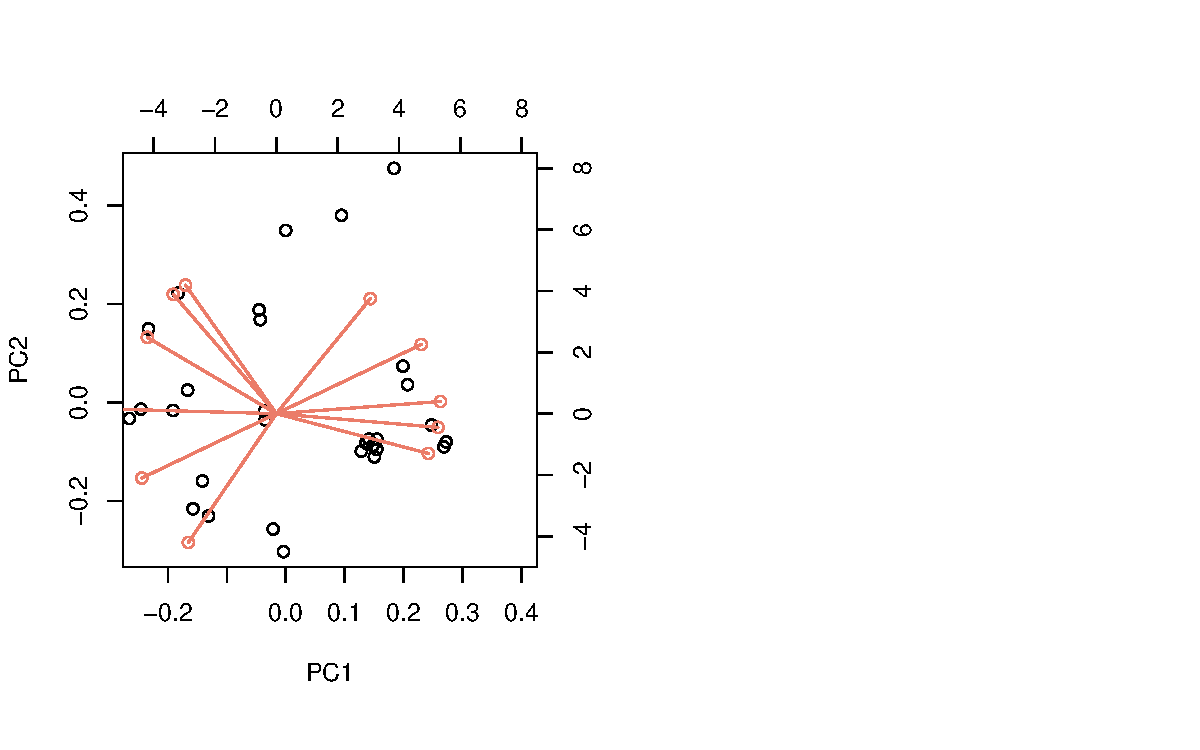
\includegraphics[width=\maxwidth]{figure/beamer-PCAbiplot-deconstruction-1} 

}

\caption[PCA biplot of mtcars dataset]{PCA biplot of mtcars dataset: mathematical construction}\label{fig:PCAbiplot-deconstruction}
\end{figure}

\end{knitrout}

\begin{knitrout}\scriptsize
\definecolor{shadecolor}{rgb}{0.969, 0.969, 0.969}\color{fgcolor}\begin{kframe}
\begin{alltt}
\hlcom{#GENERATION OF A BIPLOT WITH R'S BUILT-IN FUNCTIONS}
\hlcom{# Standardise the data}
\hlstd{scaled_data} \hlkwb{<-} \hlkwd{scale}\hlstd{(mtcars)}

\hlcom{# Perform Principal Component Analysis (PCA)}
\hlstd{pca_result} \hlkwb{<-} \hlkwd{prcomp}\hlstd{(scaled_data,} \hlkwc{scale.} \hlstd{=} \hlnum{TRUE}\hlstd{)}

\hlcom{# Create a biplot}
\hlkwd{biplot}\hlstd{(pca_result,} \hlkwc{cex} \hlstd{=} \hlnum{0.7}\hlstd{)}
\end{alltt}
\end{kframe}\begin{figure}[H]

{\centering 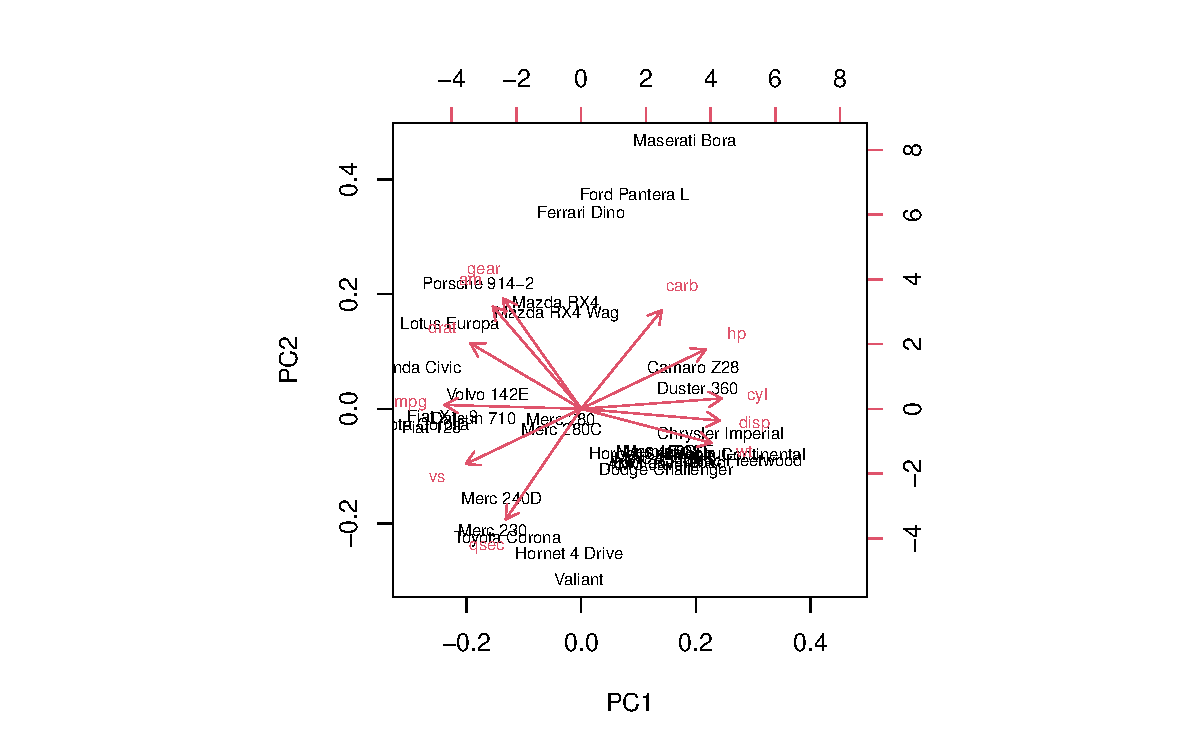
\includegraphics[width=\maxwidth]{figure/beamer-PCAbiplot-1} 

}

\caption[PCA biplot of mtcars dataset]{PCA biplot of mtcars dataset: R built-in function}\label{fig:PCAbiplot}
\end{figure}

\end{knitrout}

\noindent Comparative analysis of these two plots reveals several key findings. The manual construction approach offers meticulous control over the biplot's customisation, allowing for fine-tuning of parameters and appearance. Conversely, the in-built function approach provides a user-friendly ideal for practitioners less inclined towards mathematical intricacies the visualisation. However, despite differences in implementation, both methodologies produce visually comparable biplots, showcasing identical patterns and relationships within the data.

\subsection{Principal Curves}

\noindent Principal curves stand as a vital tool in exploratory data analysis, providing a nonlinear analogue to PCA for capturing the underlying structure of multidimensional data. While PCA focuses on finding linear projections that maximise variance, principal curves seek to identify smooth, nonlinear trajectories that capture the most significant variations in the data. These curves are essentially one-dimensional paths embedded within the multidimensional space of the data points.\\

\noindent Hence, if the points don't fall in a linear subspace, that is, they fall in a non-linear subspace such as a curve in 2-dimension, PCA is insufficient. An example of this is the scatter plot on the left side of Figure~\ref{fig:P-curves}. In this case, a straight line can't be placed in the middle of the plot, however, one could fit a curve that passes through the centre of the points. This is the purpose that principal curves serve

\subsubsection{Construction of Principal Curves}

\noindent As with PCA, take $(n \times p)$ data matrix $\mathbf{X}$, with row vectors $\mathbf{x}_i$. The goal is to extract a lower-dimensional set of "factors" or "scores" $\mathbf{y} = (y_1, \dots, y_n)^T$. These satisfy the following model:

\[
\mathbf{x}_i = f(y_i) + \epsilon_i, 
\]

\noindent where $\epsilon_i$ are errors with mean 0 and variance $\sigma^2 \mathbf{I}_p$ and $f: \mathbb{R}^1 \rightarrow \mathbb{R}^p$ is a continuous function called a curve.\\

\noindent For curve $\mathbf{f}$, the projection index $y_f(\mathbf{x})$ maps observation $\mathbf{x} \in \mathbb{R}^p$ to the point of $\mathbf{f}$ that is closest, returning the score (index). If there are several such points, it returns the largest (this is arbitrary choice to ensure it is a well defined function). Hence, the projection index is: 
\[
y_f(\mathbf{x}) = \sup\limits_{y}\{y: ||\mathbf{x}-\mathbf{f}(y)||= \inf\limits_{\mu}||\mathbf{x}-\mathbf{f}(\mu)||\}.
\]

\noindent As seen in a similar form in PCA, principal curves estimates the following least-squares objective function
\[
\min\limits_{\mathbf{f}}\sum_{i=1}^{n} ||\mathbf{x}_i - \mathbf{f}(y_{\mathbf{f}}(\mathbf{x}_i))||^2.
\]

\noindent To construct the principal curve, an algorithm put to work. This iterates between finding a curve $\mathbf{f}$ and then projecting the points onto that. More explicitly, the algorithms has the following form: %https://www.youtube.com/watch?v=lnxz3QAA1po 

\begin{enumerate}
  \item Initialise: let iteration counter $h = 1$ and set $\mathbf{y}^{(0)} = \mathbf{Xu}$, where $\mathbf{u}$ is the first PC vector. 
  \item Smoothing step: With $\mathbf{y}^{(h-1)}$ fixed, estimate $\mathbf{\hat{x}}_i^{(h)}$ with a smoother. 
  \item Projection step: With $\mathbf{\hat{X}}^{(h)}$ fixed, use the projection index to update the scores $\mathbf{y}{(h)}$ so that they have unit speed. 
  \item Loop: Increment $h$ and return to step 1 while the change in the objective function above some threshold.
\end{enumerate}

\subsubsection{Principal Cuves in Practice}

\noindent In Figure~\ref{fig:P-curves}, we see an example of how a principal curve is fitted to the observations of an artificial dataset. The points in the plots are not grouped in a linear subspace, but rather follow a similar shape to that of cubic function.\\

\noindent Using the built-in \texttt{principal-curve()} function, a principal curve can be fitted to the dataset. The principal curve traverses through the densest regions of the data distribution, capturing the underlying nonlinear structure. The panel on the left of Figure~\ref{fig:P-curves} depicts the principal curve overlaid on the dataset, providing insights into the central tendency and inherent curvature of the data. Additionally, whiskers are drawn to visualise the perpendicular distances between data points and the principal curve.

\begin{knitrout}\scriptsize
\definecolor{shadecolor}{rgb}{0.969, 0.969, 0.969}\color{fgcolor}\begin{figure}[H]

{\centering 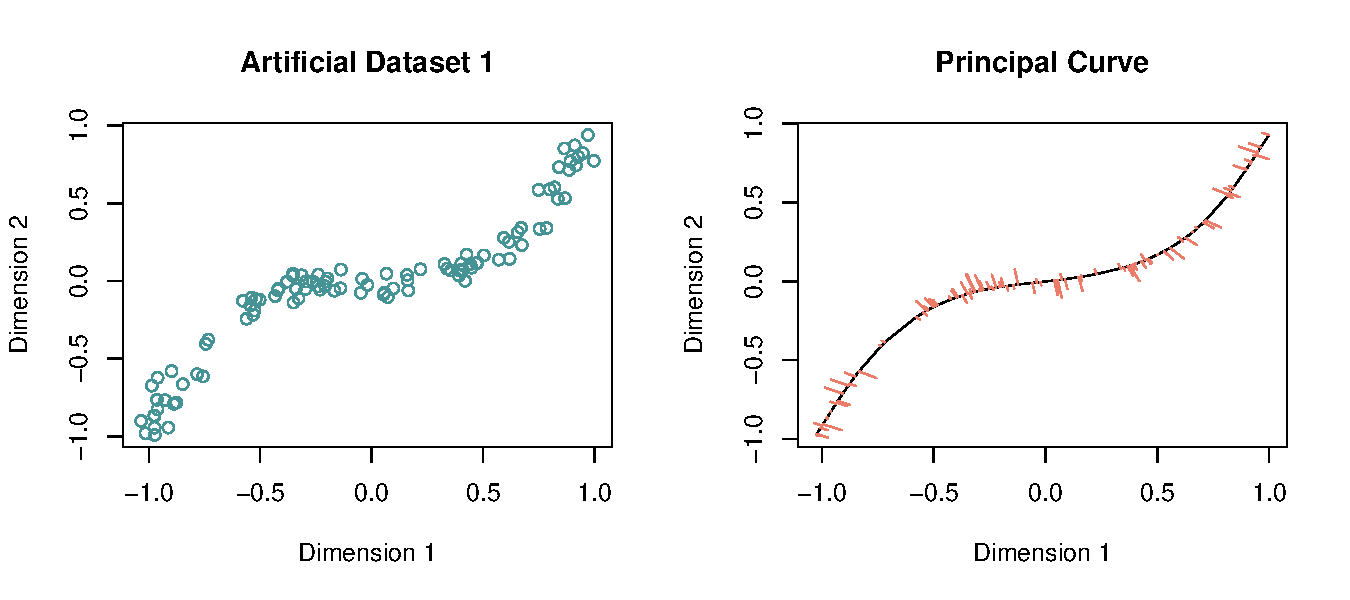
\includegraphics[width=\maxwidth]{figure/beamer-P-curves-1} 

}

\caption[Principal curve fitting illustration on artificial dataset]{Principal curve fitting illustration on artificial dataset}\label{fig:P-curves}
\end{figure}

\end{knitrout}

\noindent The principal curve effectively captures the nonlinear relationship between the dimensions of the artificial dataset. By flexibly adapting to the curvature of the data distribution, the principal curve reveals intricate patterns and trends that may not be captured by linear methods like PCA. The visualisation aids in understanding the underlying structure of the dataset.


\subsection{t-SNE}
\href{https://jmlr.org/papers/volume9/vandermaaten08a/vandermaaten08a.pdf}

\noindent
Since PCA is a linear method and may not perform well with non-linear data structures, often missing complex non-linear relationships. Although effective in capturing the global structure of data, PCA focuses on maintaining large pairwise distances to maximise variance and overlook important local patterns and structures. \\

\noindent
Unlike PCA, t-Distributed Stochastic Neighbor Embedding (t-SNE) is a nonlinear technique for embedding high-dimensional data for visualization in a low-dimensional space of two or three dimensions, focusing on preserving the small pairwise similarities between data points thus retain the local structure of the dataset in a lower-dimensional space. It starts by converting high-dimensional Euclidean distances into probabilities that reflect the similarity between points, then maps these points to a lower-dimensional space in a way that tries to preserve these similarities.\\

\noindent
First, for each pair of high-dimensional points $x_i$ and $x_j$, the similarity between data points is quantified using conditional probabilities $p_{j|i}$, that $x_i$ would choose $x_j$ as its neighbor if neighbors were picked in proportion to thier probability density under a Gaussian centred at $x_i$. Mathematically, the conditional probability $p_{j|i}$ is given by:
    \[
        p_{j|i} = \frac{\exp(-||\mathbf{x}_i - \mathbf{x}_j||^2 / 2\sigma_i^2)}{\sum_{k \neq i}\exp(-||\mathbf{x}_i - \mathbf{x}_k||^2 / 2\sigma_i^2)}.
    \] \\

\noindent
Then, the joint probability distribution $P$ in the high-dimensional space is symmetrized as follows:
    \[
        p_{ij} = \frac{p_{j|i} + p_{i|j}}{2N},
    \] \\
\noindent
where $N$ is a number of dimensions.\\

\noindent
In the low-dimensional space, t-SNE alleviates the crowding problem, which is a common issue in methods like PCA (Principal Component Analysis). It does so by using a t-distribution in the low-dimensional space, which has heavier tails than a Gaussian distribution. t-SNE calculates similar probabilities using a Student's t-distribution:
    \[
        q_{ij} = \frac{(1 + ||\mathbf{y}_i - \mathbf{y}_j||^2)^{-1}}{\sum_{k \neq l}(1 + ||\mathbf{y}_k - \mathbf{y}_l||^2)^{-1}}.
    \] \\
    
\noindent
The objective is to minimise the Kullback-Leibler divergence between the joint probability distributions $P$ and $Q$:
    \[
        C = \text{KL}(P || Q) = \sum_{i \neq j} p_{ij} \log \frac{p_{ij}}{q_{ij}},
    \] \\
\noindent
where the $C$ means the cost function, and the Kullback-Leibler (KL) divergence is a measure of how one probability distribution diverges from a second, reference probability distribution. In addition, the lower the KL divergence value, the closer the two distributions are. A KL divergence of zero means that these two distributions are the same.\\

\noindent
This process is achieved through gradient descent. The gradient of symmetric SNE is fairly similar to that of asymmetric SNE, and is given 
\[
        \partial C = \text{KL}(P || Q) = \sum_{i \neq j} p_{ij} \log \frac{p_{ij}}{q_{ij}}.
    \] \\
    
\noindent
Perplexity influences the variance of the Gaussians in the high-dimensional space and is a crucial hyperparameter in t-SNE.\\

\noindent \textbf{t-SNE in Practice}\\

\noindent
R provides us with a dedicated package for t-SNE analysis, \textit{Rtsne}, which allows us to conduct the analysis conveniently using the \textit{Rtsne} function. In the graph presented below, we observe a t-SNE visualization of the penguin dataset.\\
\\

\begin{knitrout}\scriptsize
\definecolor{shadecolor}{rgb}{0.969, 0.969, 0.969}\color{fgcolor}\begin{figure}[H]

{\centering 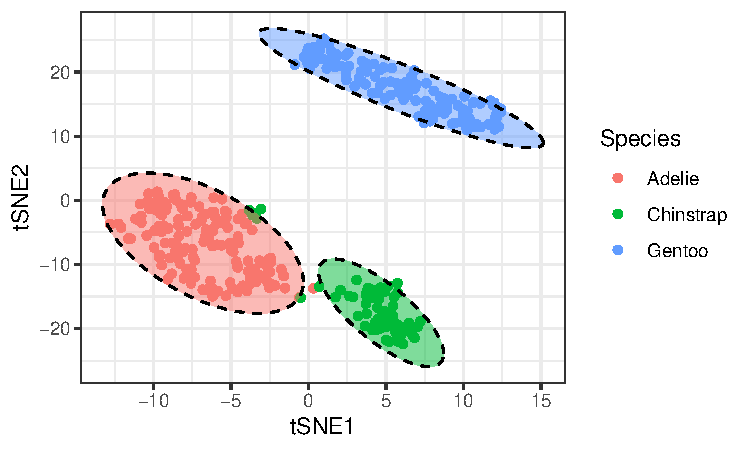
\includegraphics[width=\maxwidth]{figure/beamer-t-SNE-1} 

}

\caption[t-SNE of Penguins Dataset]{t-SNE of Penguins Dataset}\label{fig:t-SNE}
\end{figure}

\end{knitrout}


\noindent
The provided plot in Figure~\ref{fig:t-SNE} is a t-SNE visualization of the Penguins dataset, rendered using the $ggplot2$ package in R. In this case, using the T-sne algorithm helps us to reduce the multidimensional numerical data of the penguin dataset to a $2$-dimensional space. We also use scatter plots and elliptical areas to visualize the distribution of different penguin species. The data points are colour-coded to distinguish between three penguin species: Adelie in red, Chinstrap in green, and Gentoo in blue. This colour coding aids in the visual differentiation of the species clusters.\\

\noindent
The axes are labeled $tSNE1$ and $tSNE2$, corresponding to the dimensions reduced by the t-SNE algorithm. Dashed ellipses overlaid on the scatter plot demarcate the clusters of each species, providing a visual guide to the density and separation of the species within the transformed feature space. The plot effectively uses the t-SNE technique to illustrate the grouping of species, highlighting the algorithm's utility in discerning inherent data patterns in a lower-dimensional representation.\\

\noindent
While t-SNE is an exceptionally potent tool for data visualization, it does come with its own set of constraints. Firstly, it has a significant memory footprint and can be time-consuming to run, which may pose challenges when dealing with large datasets.\\

\noindent
Secondly, t-SNE is tailored specifically for visualization, which constrains the embedding space to two or three dimensions. This limitation means that t-SNE is optimised for human interpretability rather than for capturing higher-dimensional relationships.\\

\noindent
Additionally, it requires experimentation with different initializations to mitigate the risk of local suboptimal solutions affecting the results. Therefore, it's crucial to carefully consider and select the most suitable method based on the specific requirements and nature of the data at hand.\\

\newpage 

\section{State-Of-The-Art Modern Approaches}
Data visualisation plays a pivotal role in modern mathematics, aiding researchers and practitioners in gaining insights from complex datasets.  

\subsection{Box Plots}

\noindent Box plots, also known as box-and-whisker plots, were introduced by John W. Tukey in 1977 as a robust method for representing the distribution of a dataset. Over the years, box plots have become a staple in exploratory data analysis, offering a concise summary of the central tendency, spread, and skewness of a dataset. Traditional box plots display the median, quartiles, and any potential outliers, making them effective for comparing multiple datasets and identifying patterns within each.


\begin{knitrout}\scriptsize
\definecolor{shadecolor}{rgb}{0.969, 0.969, 0.969}\color{fgcolor}\begin{figure}[h]

{\centering 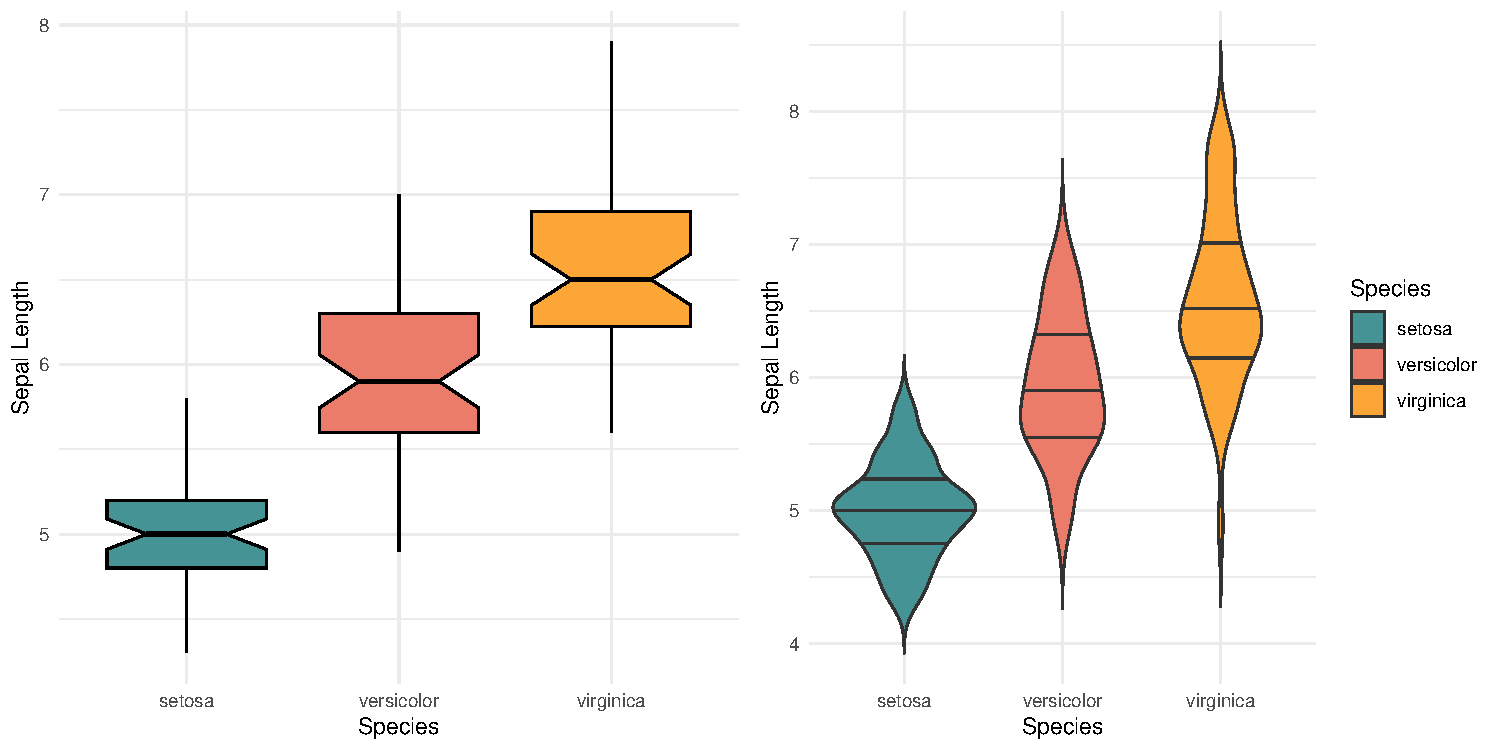
\includegraphics[width=\maxwidth]{figure/beamer-box-plots-1} 

}

\caption[Comparison of Violin and Box Plots of Sepal Length by Species]{Comparison of Violin and Box Plots of Sepal Length by Species}\label{fig:box-plots}
\end{figure}

\end{knitrout}

\noindent Recent advancements in box plot techniques include variations such as violin plots, found on the right side of Figure~\ref{fig:box-plots}, and modified box plots that incorporate additional statistical measures. These adaptations enhance the interpretability and utility of box plots across diverse applications, making them more versatile for researchers and data analysts.

\subsection{Functional Box Plots}

\noindent Functional data analysis (FDA) extends traditional statistical methods to handle functional data, where the observations are curves or functions rather than single values. Functional box plots were introduced as an extension of box plots to accommodate the unique challenges posed by functional data. Developed by Hadley Wickham and Dianne Cook in 2011, functional box plots offer a visual representation of the central tendency, spread, and shape of a distribution for functional datasets.

\noindent Functional box plots have found applications in various fields, such as biology, finance, and signal processing, where researchers deal with data in the form of curves or functions. The incorporation of concepts such as depth functions and band depth in functional box plots has improved their robustness and made them suitable for analyzing complex functional datasets.

\subsubsection{Functional Box Plot Example}
XXXX

\subsection{Quantile-Quantile Plots}

\noindent Quantile-Quantile (QQ) plots represent a powerful and widely utilised approach in exploratory data analysis and statistical inference, offering insightful visualisations of the similarity between two probability distributions. In section, the essence of QQ plots, their generation, the information they convey, and their relevance in contemporary data visualisation methodologies are explored.\\

\noindent QQ plots are constructed by plotting the quantiles of two datasets against each other. Typically, one dataset serves as the basis for theoretical quantiles, often assumed to follow a particular probability distribution, while the other dataset comprises observed values. This comparative depiction enables a direct assessment of how closely the observed data align with the theoretical distribution, facilitating the identification of deviations from expected patterns.

\subsubsection{QQ-Plots in Practice}\\
\noindent In this section, side-by-side QQ plots are displayed offering a visual comparison of the distributional properties of two variables from the mtcars and the iris datset. These plots serve as a means to assess normality assumptions and identify potential deviations from expected distributions. Through this visual exploration, we aim to gain insights into the underlying structure of the data and guide further investigation.

\begin{knitrout}\scriptsize
\definecolor{shadecolor}{rgb}{0.969, 0.969, 0.969}\color{fgcolor}\begin{figure}[h]

{\centering 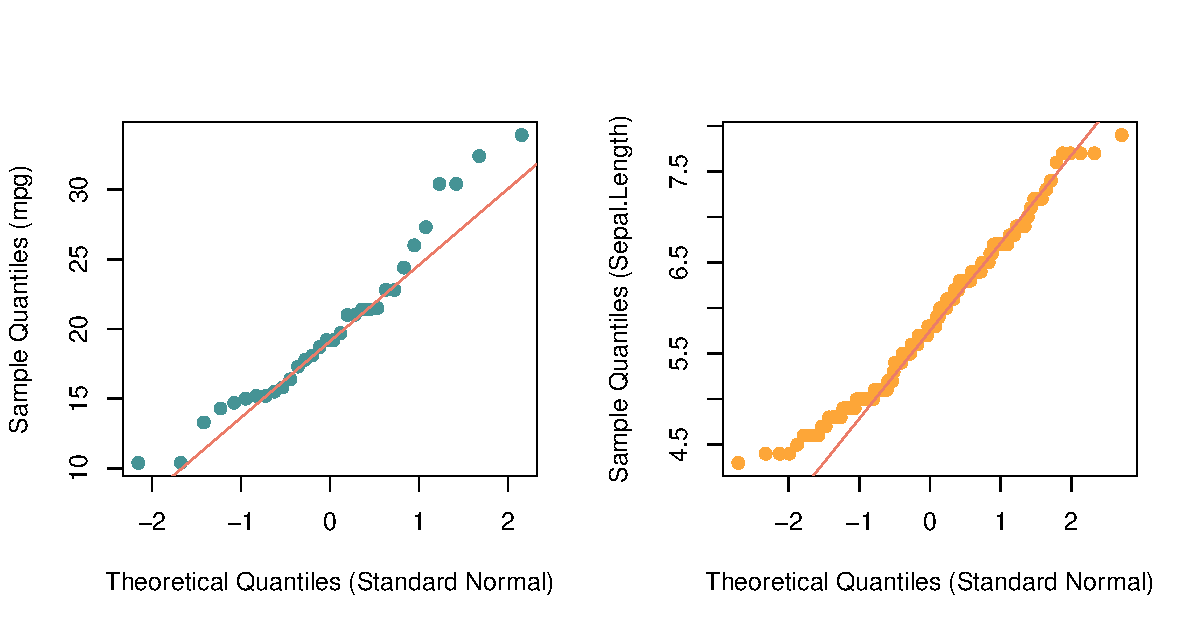
\includegraphics[width=\maxwidth]{figure/beamer-QQplots-1} 

}

\caption[Q-Q plot of mpg in mtcars dataset]{Q-Q plot of mpg in mtcars dataset}\label{fig:QQplots}
\end{figure}

\end{knitrout}

\noindent In the first plot in Figure~\ref{fig:QQplots}, which examines the mpg variable in the mtcars dataset, the points closely adhere to the theoretical quantiles line, indicating a relatively normal distribution. However, there are subtle deviations observed, particularly in the tails of the distribution, suggesting potential departures from normality. The deviations might indicate the presence of outliers or non-normal behavior in the data, which warrants further investigation.\\

\noindent Conversely, the second plot explores the distribution of the Sepal.Length variable in the iris dataset. Here, the points exhibit a clearer departure from the theoretical quantiles line compared to the mpg plot. The deviation is more pronounced, particularly towards the upper quantiles, indicating a non-normal distribution. This departure could be attributed to the presence of distinct subgroups or underlying factors influencing the distribution of sepal lengths within the iris dataset.\\

\noindent In general, the QQ plots provide a succinct and insightful representation of the distributional properties of the variables under examination. They offer a visual means to assess normality assumptions and identify potential outliers or deviations from expected distributions. As such, QQ plots serve as a valuable tool in exploratory data analysis and model diagnostics, aiding researchers in understanding the underlying structure of their data and guiding subsequent analyses.


\newpage  

\section{Index}  

\begin{itemise}
    \item \textbf{Accuracy}: Emphasising faithful reflection of data to reduce distortion or misinterpretation.
    \item \textbf{Clarity}: Ensuring visuals are easily understood without unnecessary complexity.
    \item \textbf{Cognitive Load}: The mental effort required to process information presented visually.
    \item \textbf{Cognitive psychology}: Understanding how mental processes affect perception and understanding of visual data.
    \item \textbf{Colour Theory}: Principles guiding the strategic use of colour in visualisations for clarity and impact.
    \item \textbf{Colour encoding}: Utilising colours to represent data categories or values in visualisations.
    \item \textbf{Colour perception}: Understanding how humans perceive and interpret colours in visualisations.
    \item \textbf{Consistency}: Maintaining uniform use of visual elements throughout a visualisation.
    \item \textbf{Data abstraction}: Simplifying and structuring raw data into comprehensible visual forms.
    \item \textbf{Gestalt Principles}: Rules affecting how visual elements are grouped and interpreted in perception.
    \item \textbf{Hierarchies of abstraction}: Representing data at various levels of detail in visualisation.
    \item \textbf{Information overload}: Occurs when excessive data or visual elements overwhelm understanding.
    \item \textbf{Interval data}: Ordered categories with equal intervals but lacking a true zero point.
    \item \textbf{Nominal data}: Represents categories or labels without any inherent order.
    \item \textbf{Ordinal data}: Implies a meaningful order among categories but lacks equal intervals.
    \item \textbf{Ratio data}: Includes ordered categories with equal intervals and a meaningful zero point.
    \item \textbf{Relevance}: Presenting information pertinent to the addressed message or question.
\end{itemise}
  
  

\newpage

\bibliographystyle{plain} % Choose a style that suits your needs
\bibliography{reference} % The filename of your .bib file

\end{document}
